\section{\crdtimp{}}
\label{sec:crdt implementation}



\subsection{Multi-Value Register Implementation}
\label{subsec:multi-value register implementation}

\cite{ShapiroPBZ11} introduces state-based \crdtimp{}, where an update occurs entirely at the source replica, and then propagates by transmitting the modified payload between replicas. When a replica receives a effector of modified payload, it calls method {\tt merge}, which takes the current payload and the payload in effector, and returns a new payload. \cite{ShapiroPBZ11} shows how to obtain a operation-based \crdtimp{} from a state-based \crdtimp{}, and we draw it in Listing~\ref{lst:operation-based emulation of state-based object}. Since query operations do not change, we ignore query operations. To do a update operation $f(a)$, we compute the state-based update and perform merge in downstream. Here the precondition of downstream is empty because merge is always enabled.


\begin{minipage}[t]{1.0\linewidth}
\begin{lstlisting}[frame=top,caption={operation-based emulation of state-based object},
captionpos=b,label={lst:operation-based emulation of state-based object}]
  payload S ( the state-based payload )
  initial initial payload of S

  f(a)
    atSource :
      precondition : precondition of f(a)
      let s = atSource of f(a) in state-based
    downStream(s) :
      S = merge(S,s)
\end{lstlisting}
\end{minipage}

$\\$ $\\$

\cite{ShapiroPBZ11} gives a state-based multi-value register implementation. As discussed above, we give its operation-based version in Listing~\ref{lst:operation-based multi-value register}. Here $\alabelshort[{\tt myRep}]{}$ is a function that returns current replica identifier. This implementation assumes that the number of replicas are fixed. A payload $S$ is a set of $(a,V)$ pairs, where $a$ is a value and $V$ is a vector called version vector. The size of $V$ is the number of replicas in distributed system. %Annotation1 is an annotation for the current payload, and annotation2 is an annotation for downstream of $write(a)$.
Given vector clock $V$ and $V'$, we say that $V > V'$, if for each replica $\arep$, we have $V[\arep] > V'[\arep]$. Annotation1 is an annotation for effector of $write(a)$.


\begin{figure}[t]
\begin{lstlisting}[frame=top,caption={Pseudo-code of operation-based multi-value register},
captionpos=b,label={lst:operation-based multi-value register}]
  payload Set S
  initial S = @|$\emptyset$|@
  initial lin = @|$\epsilon$|@

  write(a) :
    atSource :
      let g = myRep()
      let @|$\mathcal{V}$|@ = @|$\{ V \vert \exists x, (x,V) \in S \}$|@
      let @|$V'$|@ = @|$[ max_{V \in \mathcal{V}} V[j]]_{j \neq g}$|@
      let @|$V'[g]$|@ = @|$max_{V \in \mathcal{V}} V[g]$|@ + 1
      //@ lin = lin@|$\,\cdot\,( $|@readIds()@|$\,\Rightarrow\,$|@S@|$ )\,\cdot\,write(a,V',S)$|@
    downStream(@|$(a,V')$|@) :
      let A = @|$\{ (a_1,V_1) \in S \vert \neg V' > V_1 \}$|@
      let B = @|$\{ (a,V') \}$|@, if @|$\forall (a_1,V_1) \in S, \neg V_1 > V'$|@. Otherwise, let B = @|$\emptyset$|@
      S = A @|$\cup$|@ B
      //@ Annotation1 : @|$\forall \arep, V'[\arep]$|@ = @|$\vert \{ \alabel = \alabelshort[{\tt write}]{\_}, \alabel$|@ happens on replica @|$\arep,  (\alabel,\alabelshort[write]{a,V'}) \in \avisord \vee \alabel = \alabelshort[write]{a,V'} \} \vert$|@

  read() :
    let @|$S_1$|@  = {a : @|$\exists$|@ V. (a,V) @|$\in$|@ S}
    //@ lin = lin@|$\,\cdot\,( $|@read()@|$\,\Rightarrow\,S_1)$|@
    return @|$S_1$|@
\end{lstlisting}
\end{figure}

%//@ Annotation1 : S =  @|$\{ (a,V) \vert \exists \alabel = \alabellongind[write]{a,V}{\bot}{*}, \alabel$|@ is maximal w.r.t @|$\avisord$|@ among write operations applied in current replica @|$\}$|@






\subsection{Counter Implementation}
\label{subsec:counter implementation}

\cite{ShapiroPBZ11} gives a operation-based counter implementation, which is shown in Listing~\ref{lst:operation-based counter}. A payload is a integer $ctr$.


\begin{figure}[t]
\begin{lstlisting}[frame=top,caption={Pseudo-code of operation-based counter},
captionpos=b,label={lst:operation-based counter}]
  payload integer ctr
  initial ctr = 0
  initial lin = @|$\epsilon$|@

  inc() :
    atSource :
      //@ lin = lin@|$\,\cdot\,inc() $|@
    downStream(inc) :
      ctr = ctr + 1

  dec() :
    atSource :
      //@ lin = lin@|$\,\cdot\,dec() $|@
    downStream(dec) :
      ctr = ctr - 1

  read() :
    //@ let lin' = lin@|$\,\cdot\,(read()\Rightarrow ctr)$|@
    return ctr
\end{lstlisting}
\end{figure}

%//@ Annotation1 : S =  @|$\{ (a,V) \vert \exists \alabel = \alabellongind[write]{a,V}{\bot}{*}, \alabel$|@ is maximal w.r.t @|$\avisord$|@ among write operations applied in current replica @|$\}$|@





\subsection{PN-Counter Implementation}
\label{subsec:PN-counter implementation}

\cite{ShapiroPBZ11} gives a state-based PN-counter implementation. As discussed above, we give its operation-based version in Listing~\ref{lst:operation-based PN-counter}. Here $\alabelshort[{\tt myRep}]{}$ is a function that returns current replica identifier, and $\alabelshort[{\tt reps}]{}$ is a function that returns the number of replicas in distributed system. This implementation assumes that the number of replicas are fixed. A payload $S$ contains a integer array $P$ and a integer array $N$. $P[\arep]$ represents the number of $\alabelshort[{\tt inc}]{}$ that happens on replica $\arep$ and their effector have been applied in current local sate, while $N[\arep]$ represents the number of $\alabelshort[{\tt dec}]{}$ that happens on replica $\arep$ and their effector have been applied in current local sate. Annotation1 is an annotation for effector of {\tt inc} or {\tt dec}.


\begin{figure}[t]
\begin{lstlisting}[frame=top,caption={Pseudo-code of operation-based PN-counter},
captionpos=b,label={lst:operation-based PN-counter}]
  payload ingeter[reps()] P, ingeter[reps()] N  
  initial P = [@|$0,\ldots,0$|@], N = [@|$0,\ldots,0$|@]
  initial lin = @|$\epsilon$|@ 
  
  inc()
    atSource : 
      let g = myRep() 
      let @|$P'$|@ = @|$P[ g: P[g] + 1]$|@ 
      let @|$N'$|@ = @|$N$|@ 
      //@ lin = lin@|$\,\cdot\,inc()$|@ 
    downStream(@|$(P',N')$|@) :
      @|$\forall \arep$|@, @|$P[\arep]$|@ = @|$max( P[\arep],P'[\arep] )$|@ 
      @|$\forall \arep$|@, @|$N[\arep]$|@ = @|$max( N[\arep],N'[\arep] )$|@
      //@ Annotation1 : @|$\forall \arep, P'[\arep]$|@ = @|$\vert \{ \alabel = \alabelshort[{\tt inc}]{}, \alabel$|@ happens on replica @|$\arep,  (\alabel,\alabel') \in \avisord \vee \alabel = \alabel', where \ \alabel'$|@ is the operation that generate this @|$(P',N')$|@ effector @|$\} \vert$|@, 
      @|$N'[\arep]$|@ = @|$\vert \{ \alabel = \alabelshort[{\tt dec}]{}, \alabel$|@ happens on replica @|$\arep,  (\alabel,\alabel') \in \avisord \vee \alabel = \alabel', where \ \alabel'$|@ is the operation that generate this @|$(P',N')$|@ effector @|$\} \vert$|@, 
  
  dec()
    atSource :
      let g = myRep()
      let @|$P'$|@ = @|$P$|@
      let @|$N'$|@ = @|$N[ g: N[g] + 1]$|@
      //@ lin = lin@|$\,\cdot\,dec()$|@
    downStream(@|$(P',N')$|@) :
      @|$\forall \arep$|@, @|$P[\arep]$|@ = @|$max( P[\arep],P'[\arep] )$|@
      @|$\forall \arep$|@, @|$N[\arep]$|@ = @|$max( N[\arep],N'[\arep] )$|@
      //@ Annotation1 : @|$\forall \arep, P'[\arep]$|@ = @|$\vert \{ \alabel = \alabelshort[{\tt inc}]{}, \alabel$|@ happens on replica @|$\arep,  (\alabel,\alabel') \in \avisord \vee \alabel = \alabel', where \ \alabel'$|@ is the operation that generate this @|$(P',N')$|@ effector @|$\} \vert$|@,
      @|$N'[\arep]$|@ = @|$\vert \{ \alabel = \alabelshort[{\tt dec}]{}, \alabel$|@ happens on replica @|$\arep,  (\alabel,\alabel') \in \avisord \vee \alabel = \alabel', where \ \alabel'$|@ is the operation that generate this @|$(P',N')$|@ effector @|$\} \vert$|@,
      

  read() :
    let c  = @|$\Sigma_{\arep} P[\arep]$|@ - @|$\Sigma_{\arep} N[\arep]$|@
    //@ lin = lin@|$\,\cdot\,\alabellongind[{\tt read}]{}{c}{}$|@
    return c
\end{lstlisting}
\end{figure}

%//@ Annotation1 : S =  @|$\{ (a,V) \vert \exists \alabel = \alabellongind[write]{a,V}{\bot}{*}, \alabel$|@ is maximal w.r.t @|$\avisord$|@ among write operations applied in current replica @|$\}$|@







\subsection{The Wooki Algorithm}
\label{subsec:the Wooki algorithm}

The Wooki algorithm of \cite{DBLP:conf/wise/WeissUM07} is given in Listing~\ref{lst:wooki algorithm}. %Note that here $integrateIns$ is a recursive method used by $addBetween$ method.
Wooki algorithm is an optimized version of Woot \cite{DBLP:conf/cscw/OsterUMI06}. To make our introduction more clear, we borrow the notion of W-character and W-string from Woot algorithm.

In local state of each replica, Wooki algorithm stores the list as a sequence of W-characters. A W-character $w$ is a tuple $(id,v,degree,flag)$, where $id$ is the identifier of $w$; $v$ is the value of $w$; $degree$ is the degree of $w$; $flag \in \{ \mathit{true},\mathit{false} \}$ is the flag of $w$ and indicates whether $w$ is ``visible'' in list. A identifier $id$ of W-character is a unique timestamp. %tuple $(ctr,\arep)$, where $ctr \in \mathbb{N}$.
We use $degree(c)$ to denote the degree of $c$.

A W-string is an ordered sequence of W-characters $w_{begin} \cdot w_1 \cdot \ldots \cdot w_n \cdot w_{end}$, where $w_{begin}$ and $w_{end}$ are special W-characters that mark the beginning and the ending of the sequence. The values of $w_{begin}$ and $w_{end}$ are $\circ_{begin}$ and $\circ_{end}$, respectively. The degree of $w_{begin}$ and $w_{end}$ are $0$. We define the following function for a W-string $str$:

\begin{itemize}
\setlength{\itemsep}{0.5pt}
\item[-] $\vert str \vert$ returns the length of $str$,

\item[-] $str[p]$ returns the W-character at position $p$ in $str$. Her we assume that the first element of $str$ is at position 0.

\item[-] $pos(str,w)$ returns the position of W-character $w$ in $S$.

\item[-] $insert(str,w,p)$ inserts W-character $w$ into $str$ at position $p$.

\item[-] $subseq(str,w_1,w_2)$ returns the part of $str$ between the W-characters $w_1$ and $w_2$ (excluding $w_1$ and $w_2$).

\item[-] $contains(str,a)$ returns true if there exists a W-character in $str$ with value $a$.

\item[-] $values(str)$ returns the sequence of visible (with $\mathit{true}$ flag) values of $str$.

\item[-] $getWchar(str,a)$ returns the W-character with value $a$ in $str$.

\item[-] $changeFlag(str,pos,f)$ changes the flag of $str[pos]$ into $f$.
\end{itemize}

%Note that only $values(str)$ distinguish whether a W-character is with flag $\mathit{true}$ or with flag $\mathit{false}$.

A total order $<_{id}$ is given for identifiers of W-characters for conflict resolution ($<_{id}$ is just the total order of timestamp). Given a W-string $str$ and two W-characters $w_1,w_2$ of $str$, we write $w_1 <_{str} w_2$ to indicate that $pos(str,w_1) < pos(str,w_2)$.

%A total order $<_{id}$ is given for identifiers of W-characters for conflict resolution. Given two identifiers $(ctr_1,\arep_1)$ and $(ctr_2,\arep_2)$, we have $(ctr_1,\arep_1) <{id} (ctr_2,\arep_2)$, if $\arep_1 < \arep_2 \vee (\arep_1 = \arep_2 \wedge ctr_1 < ctr_2)$. Given a W-string $str$ and two W-characters $a,b$ of $str$, we write $a <_{str} b$ to indicate that $pos(str,a) < pos(str,b)$.

\begin{figure}[t]
\begin{lstlisting}[frame=top,caption={Pseudo-code of Wooki algorithm},
captionpos=b,label={lst:wooki algorithm}]
  payload W-string @|$string_s$|@
  initial @|$string_s$|@ = @|$\epsilon$|@
  initial lin = @|$\epsilon$|@

  addBetween(a,b,c) :
    atSource :
      precondition :  @|$contains(string_s,a) \wedge contains(string_s,c) \wedge pos(string_s,c) > pos(string_s,a) \wedge \neg contains(string_s,b)$|@
      let ts = getTimestamp()
      let @|$w_p$|@ = @|$getWchar(string_s,a)$|@
      let @|$w_n$|@ = @|$getWchar(string_s,c)$|@
      //@ lin = lin@|$\,\cdot\,addBetween(a,b,c)$|@
    downStream((w,@|$w_p$|@,@|$w_n$|@)) : with @|$w = (ts, a, max(degree(w_p),degree(w_n)) +1, \mathit{true})$|@
      integrateIns(@|$w_p,w,w_n$|@)

  remove(a) :
    atSource :
      precondition : @|$contains(string_s,a)$|@
      let w = @|$getWchar(string_s,a)$|@
      //@ lin = lin@|$\,\cdot\,remove(a)$|@
    downStream(w) :
      let p = @|$pos(string_s,w)$|@
      @|$changeFlag(string_s,p,\mathit{false})$|@

  read() :
    let s = @|$values(string_s)$|@
    //@ lin = lin@|$\,\cdot\,(read()\Rightarrow s)$|@
    return s

  integrateIns(@|$w_p,w,w_n$|@)
    let @|$S$|@ = @|$string_s$|@
    let @|$S'$|@ = @|$subseq(S,w_p,w_n)$|@
    if @|$S' = \epsilon$|@
      then  @|$insert(S,w,pos(S,w_n))$|@
    else
      Let i = 0
      Let @|$d_{min}$|@ be the minimal degree of W-characters in @|$S'$|@
      Let F be the projection of @|$S'$|@ into W-characters with degree @|$d_{min}$|@
      if (@|$w<_{id} F[0]$|@)
        integrateIns(@|$w_p,w,F[0]$|@)
      else
        while (@|$i < \vert F \vert -1 \wedge F[i] <_{id} w$|@) do
            i = i+1
        if (@|$i = \vert F \vert -1 \wedge F[i] <_{id} w$|@)
            integrateIns(@|$F[i],w,w_n$|@)
        else
            integrateIns(@|$F[i-1],w,F[i]$|@)
\end{lstlisting}
\end{figure}

$\\$ $\\$

The payload of each replica is a W-string $string_s$.

To do $\alabelshort[{\tt addBetween}]{a,b,c}$, we first ensure that $a$ and $c$ are in $string_s$, $a$ is before $c$ in $string_s$, and $b$ is not in $string_s$. Then, we generate a W-character $w$ for value $b$, and calls method $integrateIns(w_p,w,w_n)$ to put $w$ between $w_p$ and $w_n$, which are the W-characters of $a$ and $c$ in $string_s$, respectively.

$integrateIns(w_p,w,w_n)$ is a recursive method and works as follows: If there are no W-character between $w_p$ and $w_n$, then $w$ is put after $w_p$. Else, Wooki selects a sequence $F$ of W-characters, such that each W-character of $F$ is between $w_p$ and $w_n$, and has minimal degree. It can be proved that W-characters in $F$ are sorted by the $<_{id}$ order. Then, we choose the position of $w$, and recursive call $integrateIns(w_x,w,w_y)$ for some $w_x,w_y \in F \cup \{ w_p,w_n \}$. We can see that, the minimal degree of the sub-sequence of $S$ between $w_x$ and $w_y$ is larger than that of the sub-sequence of $S$ between $w_p$ and $w_n$.

To do $\alabelshort[{\tt remove}]{a}$, we just set the flag of W-character of $a$ in $string_s$ to be $\mathit{false}$. To do ${\tt read}$, we return $values(string_s)$.





\subsection{The Tree-Doc Algorithm}
\label{subsec:the Tree-Doc algorithm}

The tree-doc algorithm of \cite{DBLP:conf/icdcs/PreguicaMSL09,DBLP:journals/corr/abs-0710-1784} is given in Listing~\ref{lst:Tree-Doc algorithm}. The tree-doc algorithm of Listing~\ref{lst:Tree-Doc algorithm} can be considered as the tree-doc with ``unique disambiguator'' in \cite{DBLP:conf/icdcs/PreguicaMSL09,DBLP:journals/corr/abs-0710-1784}, and we do not consider optimizations, such as balancing tree.

In local state of each replica, tree-doc algorithm stores the list as a set of T-characters. A T-character $w$ is a tuple $(v,tid,gv)$, where $v$ is the value of $w$, and $tid$ is a T-identifier of $w$. Here $gv$ is a ``ghost field'' of $w$ and also stores the value of $w$. The reason of introducing $gv$ is that, the $\alabelshort[{\tt remove}]{a}$ method will find the T-character $w$ of value $a$ and set the value of $w$ into a special value $nil$; while in the proof, it will be convenient if we can always remember the value of $w$. Therefore, when $w$ is initialized, the value of $w$ is put both in $v$ and $gv$, while the value in $gv$ is never changed afterward.

T-identifiers are the unique identifiers of T-characters. The requirement of T-identifier are as follows: there should be a total order $<_t$ over the T-identifiers, and the T-identifiers are designed to satisfy a ``dense'' property: for each T-identifier $tid_1,tid_2$, assume $tid_1 <_t tid_2$, then, there must exists a T-identifier $tid_3$, such that $tid_1 <_t tid_2 <_t tid_3$.

To satisfy this ``dense'' property, intuitively, tree-doc algorithm uses paths of a binary tree as T-identifier, and the order $<_t$ can be considered as ``walking the tree in infix order''. However, this is insufficient for concurrent edit, as users might concurrently insert two different T-character at the same position of a binary tree. To address this issue, when there are multiple T-character ``at a same position of the binary tree'', we call the set of these T-characters a major node, and call each of them a minor node.

For example, \autoref{fig:an execution of tree-doc, the local state of replica r1 after execution, and the T-identifiers of T-characters} shows an execution of tree-doc. Let $w_a,\ldots,w_k$ be the W-character of $a,\ldots,k$. We can see that $w_b,w_c,w_d$ are all inserted as ``left son'' of $w_a$. Therefore, the set of T-characters of $w_a,w_b,w_c$ are a major node and we use a box containing $w_a,w_b,w_c$ to emphasize a major node. Similarly, the set of T-characters of $w_e$ and $w_f$, $w_g$ and $w_h$, $w_j$ and $w_k$ are also major nodes, respectively.


\begin{figure}[t]
  \centering
  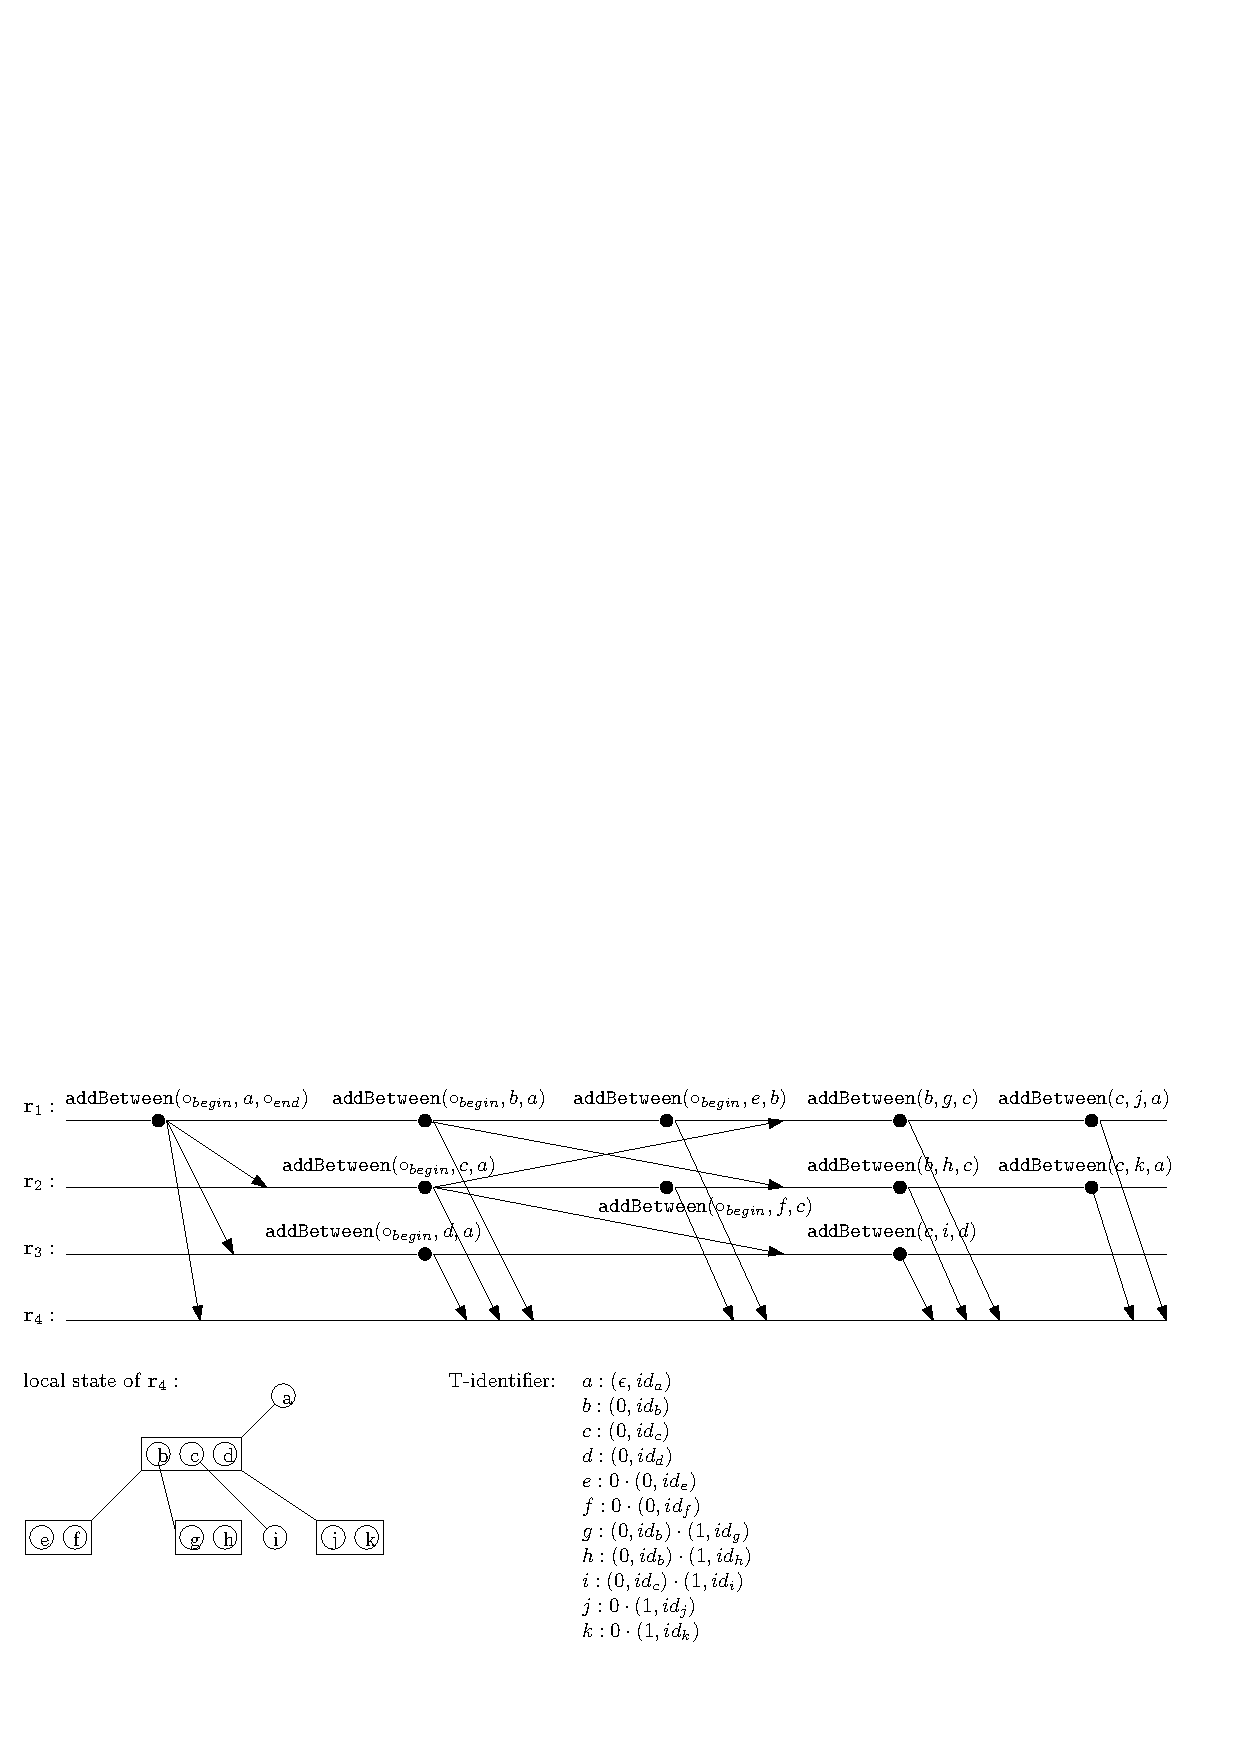
\includegraphics[width=0.8 \textwidth]{figures/TreeDocExecutionandLocalState.pdf}
\vspace{-10pt}
  \caption{An execution of tree-doc, the local state of replica $\arep_1$ after execution, and the T-identifiers of T-characters.}
  \label{fig:an execution of tree-doc, the local state of replica r1 after execution, and the T-identifiers of T-characters}
\end{figure}


A T-identifier $tid$ of a T-character $w$ is a sequence $tid = c_1 \cdot \ldots \cdot c_n \cdot (p,id)$, where $id$ is a unique identifier, and each for each $1 \leq i \leq n$, $c_i \in \{ 0,1,(1,id')\}$. We call such $id$ the disambiguator of $w$, and require disambiguator to be unique for each T-character. Each $c_i$ of $tid$ represent how to choose the next node in the $i$-th step of the ``path''. If $c_i=0$ (resp., $c_i=1$), then the next node is a node as ``left son'' (resp., ``right son'') of the current (major) node; Else, $c_i = (1,id')$, and this represents that the next node is chosen from ``right sons'' of a minor node with identifier $id'$. The path to the root is fixed to be $\epsilon$.

For example, in \autoref{fig:an execution of tree-doc, the local state of replica r1 after execution, and the T-identifiers of T-characters}, the T-identifier of $w_f$ is $0 \cdot (0,id_f)$, which represent that $w_f$ is a ``left son'' of the root's ``left son (could be a major node)''; the T-identifier of $w_g$ is $(0,id_b) \cdot (1,id_g)$, which represent that $w_g$ is a ``right son'' of minor node $w_b$. Note that, as shown in \autoref{fig:an execution of tree-doc, the local state of replica r1 after execution, and the T-identifiers of T-characters}, the corresponding tree of T-characters is not a binary tree.

We say a set $T$ of T-characters is a T-tree, if:

\begin{itemize}
\setlength{\itemsep}{0.5pt}
\item[-] There exists a T-character of $T$ with T-identifier $(\epsilon,\_)$.

\item[-] Each value of T-character is unique, and each T-character has a unique disambiguator.

\item[-] For each T-character $w=(a,tid) \in T$, assume $tid = c_1 \cdot \ldots \cdot c_n \cdot (p,id)$. We require that,for each $1 \leq i \leq n$,

    \begin{itemize}
    \setlength{\itemsep}{0.5pt}
    \item[-] If $c_i \in \{ 0,1 \}$, then there exists a T-character $w' = (\_, c_1 \cdot \ldots \cdot c_{i-1} \cdot (c_i,\_) ) \in T$,

    \item[-] Else, if $c_i = (p_i,id_i)$, then there exists a T-character $w' = (\_, c_1 \cdot \ldots \cdot c_{i-1} \cdot (p_i,id_i) ) \in T$, and there exists another T-character $w'' = (\_, c_1 \cdot \ldots \cdot c_{i-1} \cdot (p_i,id'_i) ) \in T$ and $id_i < id'_i$. Or we can say, $w'$ and $w''$ is contained in a same major node, and the disambiguator of $w'$ is less that that of $w''$.
    \end{itemize}
\end{itemize}

Given a T-tree, we the order $<_t$ is defined as follows: $tid_1 <_t tid_2$, if

\begin{itemize}
\setlength{\itemsep}{0.5pt}
\item[-] If $tid_1 = c_1 \cdot \ldots \cdot c_n \cdot (p,id)$, $(tid_2 = c_1 \cdot \ldots \cdot c_n \cdot p \cdot x \cdot l) \vee (tid_2 = c_1 \cdot \ldots \cdot c_n \cdot (p,id) \cdot x \cdot l)$, and $x=1 \vee x=(1,\_)$.

\item[-] If $tid_2 = c_1 \cdot \ldots \cdot c_n \cdot (p,id)$, $tid_1 = c_1 \cdot \ldots \cdot c_n \cdot p \cdot x \cdot l$, and $x=0 \vee x=(0,\_)$.

\item[-] If $tid_1 = c_1 \cdot \ldots \cdot c_n \cdot x_1 \cdot x_2 \cdot l_1$, $tid_2 = c_1 \cdot \ldots \cdot c_n \cdot y_1 \cdot y_2 \cdot l_2$, and one of the following cases holds for some $p \in \{ 0,1 \}$ and $id,id'$:

    \begin{itemize}
    \setlength{\itemsep}{0.5pt}
    \item[-] $x_1=p$, $x_2=0$, and $y_1=(p,\_) \vee (y_1=p \wedge y_2=1)$,

    \item[-] $x_1=(p,id)$, $x_2 \cdot l_1 = \epsilon$, $y_1=(p,id')$, and $id<id'$,

    \item[-] $x_1=(p,id)$, $x_2 \neq \epsilon$, and $(y_1 = (p,id') \wedge id<id') \vee (y_1=p \wedge y_2=1)$.
    \end{itemize}
\end{itemize}

The major node's left descendant is before any minor node and its descendant in $<_t$; minor node are ordered by disambiguator in $<_t$; given minor node $n_a,n_b$ of a same major node, such that the disambiguator of $n_a$ is less than that of $n_b$, then $n_a$ and descendant of $n_a$ is before $n_b$ and descendant of $n_b$ in $<_t$; $n_a$ and descendant of $n_a$ is before the major node's right descendant in $<_t$. Here T-identifier $tid_1$ is a descendant of T-identifier $tid_2$, if $tid_2 = c_1 \cdot \ldots \cdot c_n \cdot (p,id)$, and $tid_1 = c_1 \cdot \ldots \cdot c_n \cdot p \cdot l \vee tid_1 = c_1 \cdot \ldots \cdot c_n \cdot (p,id) \cdot l$.

We define the following function for a set $tree$ of T-characters:

\begin{itemize}
\setlength{\itemsep}{0.5pt}
\item[-] $contains(tree,a)$ returns true if there exists a T-character $(\_,\_,a)$ in $tree$.

\item[-] $getTchar(tree,a)$ returns the T-character with (ghost) value $a$ in $tree$.

\item[-] $notRemoved(tree,a)$ returns true, if there exists a T-character $(a,\_,a)$ in $tree$.

\item[-] $removeTChar(tree,a)$ first find a T-character $w=(\_,\_,a)$ in $tree$, and then set the value of $w$ into $nil$.

\item[-] $values(tree)$ returns a sequence, which is obtained by walking the tree according to $<_t$ orders and consider only values of node whose value is not $nil$.
\end{itemize}





\begin{minipage}[t]{1.0\linewidth}
\begin{lstlisting}[frame=top,caption={Pseudo-code of Tree-Doc algorithm},
captionpos=b,label={lst:Tree-Doc algorithm}]
  payload Set @|$tree$|@
  initial @|$tree$|@ = @|$\emptyset$|@
  initial lin = @|$\epsilon$|@

  addBetween(a,b,c) :
    atSource :
      precondition :  @|$contains(tree,a) \wedge contains(tree,c)\wedge \neg contains(tree,b)$|@, and @|$ \neg \exists (\_,tid,\_) \in tree, tid_a <_t tid <_t tid_c$|@, where @|$tid_a$|@ and @|$tid_c$|@ are the T-identifiers of T-characters with value a and c, respectively.
      let id = getTimestamp()
      let @|$w_a$|@ = @|$getTchar(tree,a)$|@
      let @|$w_c$|@ = @|$getTchar(tree,c)$|@
      let @|$w_b$|@ = @|$(b,newID(w_a,w_c,id),b)$|@
      //@ let lin' = lin@|$\,\cdot\,\alabelshort[{\tt addBetween}]{a,b,c}$|@
    downStream(@|$w_b$|@) :
      @|$tree$|@ = @|$tree \cup \{ w_b \}$|@

  remove(a) :
    atSource :
      precondition : @|$contains(tree,a) \wedge notRemoved(tree,a)$|@
      //@ let lin' = lin@|$\,\cdot\,\alabelshort[{\tt remove}]{a}$|@
    downStream(a) :
      @|$removeTChar(tree,a)$|@

  read() :
    let s = @|$values(string_s)$|@
    //@ let lin' = lin@|$\,\cdot\,\alabellong[{\tt read}]{}{ s }{}$|@
    return s

  newID(@|$w_1,w_2,id$|@)
      precondition : @|$ \neg \exists (\_,tid,\_) \in tree, tid_1 <_t tid <_t tid_2$|@, where @|$tid_1$|@ and @|$tid_2$|@ are the T-identifiers of @|$w_1$|@ and @|$w_2$|@, respectively.
    if @|$tid_2$|@ is a descendant of @|$tid_1$|@
      assume @|$tid_2 = l_2 \cdot (p,id_2)$|@
      return @|$l_2 \cdot p \cdot (0,id)$|@
    else if @|$tid_1$|@ is a descendant of @|$tid_2$|@
      assume @|$tid_1 = l_1 \cdot (p,id_1)$|@
      return @|$l_1 \cdot p \cdot (1,id)$|@
    else if @|$tid_1 = l\cdot (p,id_1)$|@, @|$tid_2 = l\cdot (p,id_2)$|@, and @|$tid_1 < tid_2$|@
      return @|$l \cdot (p,id_1) \cdot (1,id)$|@
    else
      assume @|$tid_1 = l_1 \cdot (p,id_1)$|@
      return @|$l_1 \cdot p \cdot (1,id)$|@
\end{lstlisting}
\end{minipage}

$\\$ $\\$

The payload of each replica is a set $tree$ of T-characters.

To do $\alabelshort[{\tt addBetween}]{a,b,c}$, we first ensure that the T-identifier of $a$ and $c$ are adjacent in $tree$, and no T-character in $tree$ has value $b$. Then, we calls method $newID(w_a,w_c,id)$ to generate a new T-identifier between that of $a$ and $c$, and use this T-identifier to generate a new T-character $w_b$, and put $w_b$ into $tree$.

$newID(w_1,w_2,id)$ require that $tid_1$ and $tid_2$ are adjacent according to $<_t$, where $tid_1$ and $tid_2$ are the T-identifiers of $w_1$ and $w_2$, respectively. It will generate a T-identifier $tid'$, such that $tid_1 <_t tid' <_t tid_2$.

To do $\alabelshort[{\tt remove}]{a}$, we just set the flag of W-character of $a$ in $string_s$ to be $\mathit{false}$. To do ${\tt read}$, we return $values(string_s)$.







\section{Sequential Specifications}
\label{sec:sequential specifications} 



\subsection{The Sequential Specification of Counter}
\label{subsec:the sequential specification of counter}

The sequential specification $\specCounter$ of counter is so that $\abstates = \mathbb{Z}$, that is the state will be an integer, and the transitions are given as follows:
\[
  \begin{array}[rcl]{rcl}
    k & \specarrow{\alabellong[\mathsf{inc}]{}{}} & k+1\\
    k & \specarrow{\alabellong[\mathsf{dec}]{}{}} & k-1\\
    k & \specarrow{\alabellong[\mathsf{read}]{}{k}} & k
  \end{array}
\]

Method $\alabelshort[{\tt inc}]{}$ increase the counter by $1$. Method $\alabelshort[{\tt dec}]{}$ decrease the counter by $1$. Method $\alabellong[{\tt read}]{}{k}{}$ returns the value of the counter.



\subsection{The Sequential Specification of OR-Set}
\label{subsec:the sequential specification of or-set}

The query-update rewriting of OR-set is as follows: $\gamma( \alabelshort[{\tt remove}]{a} ) = ( \alabellong[{\tt readIds}]{a}{S}{}, \alabelshort[{\tt remove}]{a,S})$.

% \gpwarning{I still don't like the pairs for OR-Set}
Each abstract state $\abstate$ is a set of tuples $(a,id)$, where $a$ is a data and $id$ is a identifier. The sequential specification $\specOrSet$ of OR-Set is given by the transitions:
\[
  \begin{array}{rcl}
    \abstate
    & \specarrow{\alabellong[\mathtt{readIds}]{a}{S}{}}
    & \abstate\
      \begin{array}{c}
        [\text{with}\ S = \{ (a,id)\ \vert\ (a,id) \in \abstate\}]
      \end{array}\\
    \abstate &
               \specarrow{\alabelshort[\mathtt{remove}]{a,S}}
    & \abstate \setminus S \\
    \big(\ \abstate\ |\ \mathtt{id}\ \text{does not occur in } \abstate\ \big)
             & \specarrow{ \alabelshort[{\tt add}]{a,id} }
    & \abstate \cup \{ (a,\mathtt{id}) \}\\
    \abstate
    & \specarrow{\alabellong[\mathtt{read}]{a}{ S }{}}
    & \abstate\
      \begin{array}{c}
        [\text{with}\ S = \{ a\ \vert\ \exists\ \mathtt{id}, (a,\mathtt{id}) \in \abstate \}]
      \end{array}
  \end{array}
\]

Method $\alabellong[{\tt readIds}]{a}{S}{}$ returns the set of pairs with data $a$. Method $\alabelshort[{\tt remove}]{a,S}$ removes $S$ from the abstract state. Method $\alabelshort[{\tt add}]{a,id}$ puts $\{ (a,id) \}$ into the abstract state. Method $\alabellong[{\tt read}]{}{S'}{}$ returns the value of the or-set.




\subsection{The Sequential Specification of Multi-Value Register}
\label{subsec:the sequential specification of multi-value register} 

The query-update rewriting of multi-value register is as follows: $\gamma( \alabelshort[{\tt write}]{a}) = ( \alabellong[{\tt readIds}]{}{S}{}, \alabelshort[{\tt write}]{a,id,S})$.

Each abstract state $\abstate$ is a set of tuples $(a,id)$, where $a$ is a data and $id$ is a identifier. The sequential specification $\specMVReg$ of multi-value register is given by the transitions: 

\[
  \begin{array}{rcl}
    \abstate
    & \specarrow{\alabellong[\mathtt{readIds}]{}{\abstate}{}}
    & \abstate\\
    \big(\ \abstate\ |\ \mathtt{id}\ \text{does not occur in } \abstate\ \big)
             & \specarrow{ \alabelshort[{\tt write}]{a,id,S} }
    & \abstate \setminus S \cup \{ (a,\mathtt{id}) \}\\
    \abstate
    & \specarrow{\alabellong[\mathtt{read}]{}{ S }{}}
    & \abstate\
      \begin{array}{c}
        [\text{with}\ S = \{ a\ \vert\ \exists\ \mathtt{id}, (a,\mathtt{id}) \in \abstate \}]
      \end{array}
  \end{array}
\]

Method $\alabellong[{\tt readIds}]{}{S}{}$ returns the abstract state. Method $\alabelshort[{\tt write}]{a,id,S}$ removes $S$ from the abstract state and puts $\{ (a,id) \}$ into the abstract state. Method $\alabellong[{\tt read}]{}{S'}{}$ returns the value of multi-value register.




\subsection{The Sequential Specification of List with Add-After Interface}
\label{subsec:the sequential specification of list with add-after interface} 

Each abstract state $\abstate = (l,T)$ contains a sequence $l$ of elements of a given type and a set $T$ of elements appearing in the list. The element $l$ is the list of all input values, whether already removed or not; while $T$ stores the removed values and is used as \emph{tombstone}. The sequential specification $\specRGA$ of list with add-after interface is given with the transitions as follows:
\[
  \begin{array}{rcl}
    \big(\ (l_1 \cdot a_k \cdot l_2,T\big)\ |\ a\text{ is fresh}\ \big)
     & \specarrow{\alabelshort[\mathtt{addAfter}]{a_k,a}}
     & (l_1 \cdot a_k \cdot a \cdot l_2,T)\\
     \big(\ (l,T)\ |\ a_k\ \text{occurs in}\ l\ \big)
     & \specarrow{\alabelshort[\mathtt{remove}]{a_k}}
     & (l,T \cup \{a_k\})\\
     (l,T)
     & \specarrow{\alabellong[\mathtt{read}]{}{s}{}}
     & (l,T)\
       \left[\begin{array}{c}
           \text{with $s$ is obtained from $l$}\\
           \text{by removing the values in $T$}
       \end{array}\right]
   \end{array}
\]

Method $\alabelshort[\mathtt{addAfter}]{a_k,a}$ puts $a$ immediately after $a_k$ in $l$, assuming that each value is put into list at most once. Method $\alabelshort[\mathtt{remove}]{a_k}$ adds $a_k$ into $T$, hence removing $a_k$ from the list for subsequent calls to the $\mathtt{read}$ method. Thus, $\alabellong[\mathtt{read}]{}{s}{}$ returns the list content excluding any element appearing in $T$. Assume that the initial value of list is $(\circ,\emptyset)$, and $\circ$ is never removed. When the context is clear, in $\ensuremath{\tt read}$ operation, we will omit $\circ$ in return value.





\subsection{The Sequential Specification of List with Add-Between Interface}
\label{subsec:the sequential specification of list with add-between interface} 

Each abstract state $\abstate = (l,T)$ contains a sequence $l$ of elements of a given type and a set $T$ of elements appearing in the list. The element $l$ is the list of all input values, whether already removed or not; while $T$ stores the removed values and is used as \emph{tombstone}. The sequential specification $\specWooki$ of list with add-after interface is given with the transitions as follows:
\[
  \begin{array}{rcl}
    \big(\ (l_1 \cdot a_1 \cdot l_2 \cdot l_3 \cdot a_2 \cdot l_4,T\big)\ |\ a\text{ is fresh}\ \big)
     & \specarrow{\alabelshort[\mathtt{addAfter}]{a_1,a,a_2}}
     & (l_1 \cdot a_1 \cdot l_2 \cdot a \cdot l_3 \cdot a_2 \cdot l_4,T)\\
     \big(\ (l,T)\ |\ a\ \text{occurs in}\ l\ \big)
     & \specarrow{\alabelshort[\mathtt{remove}]{a}}
     & (l,T \cup \{a\})\\
     (l,T)
     & \specarrow{\alabellong[\mathtt{read}]{}{s}{}}
     & (l,T)\
       \left[\begin{array}{c}
           \text{with $s$ is obtained from $l$}\\
           \text{by removing the values in $T$}
       \end{array}\right]
   \end{array}
\]

Method $\alabelshort[\mathtt{addAfter}]{a_1,a,a_2}$ puts $a$ at some random position between $a_1$ and $a_2$ in $l$, assuming that each value is put into list at most once. Method $\alabelshort[\mathtt{remove}]{a}$ adds $a$ into $T$, hence removing $a$ from the list for subsequent calls to the $\mathtt{read}$ method. Thus, $\alabellong[\mathtt{read}]{}{s}{}$ returns the list content excluding any element appearing in $T$. Assume that the initial value of list is $(\circ_{begin} \cdot \circ_{end},\emptyset)$, and $\circ_{begin}$ and $\circ_{end}$ are never removed. When the context is clear, in $\ensuremath{\tt read}$ operation, we will omit $\circ_{begin}$ and $\circ_{end}$ in return value. 
























\section{Proofs of \crdtimp}
\label{sec:appendix proofs of crdt implementations}



\subsection{Obtain Permutations by Swapping Adjacent and Concurrent Operations}
\label{subsec:obtain permutations by swapping adjacent and concurrent operations}

Given two sequences $l_1,l_2$  such that $l_2$ is a permutation of $l_1$, let $\mathit{diff}(l_1,l_2) = \{ (a,b) \vert$ the order of $a$ and $b$ in $l_1$ is different from that of $l_2 \}$. Given a sequence $l$ and two elements $a$ and $b$ of $l$, let $\mathit{swap}(l,a,b)$ be a sequence obtained from $l$ by swapping $a$ and $b$. The following lemma states that, given two specification sequences $(\alabelset_1, \aseqord_1)$ and $(\alabelset, \aseqord_2)$ that are generated from a same history and both consistent with visibility relation, we can obtain $\aseqord_2$ from $\aseqord_1$ by several time of swapping adjacent pair of concurrent operations.

\begin{lemma}
\label{lemma:given two sequence consistent with visibility order, one can be obtained from the other}
Given a history $(\alabelset,\avisord)$ and two two specification sequences $(\alabelset_1, \aseqord_1)$ and $(\alabelset, \aseqord_2)$ that are both consistent with $\avisord$. If $\aseqord_1 \neq \aseqord_2$, then we can obtain $\aseqord_2$ from $\aseqord_1$ by several time of swapping adjacent pair of concurrent operations.
\end{lemma}

\begin {proof}

First, we need to prove that, if $\mathit{diff}(\aseqord_1,\aseqord_2) \neq \emptyset$, then, there exists $(\alabel_1,\alabel_2) \in \mathit{diff}(\aseqord_1,\aseqord_2)$, such that $\alabel_1$ and $\alabel_2$ are concurrent, and $\alabel_1$ and $\alabel_2$ are adjacent in $\aseqord_1$.

We prove this by contradiction. Assume $\mathit{diff}(\aseqord_1,\aseqord_2) \neq \emptyset$, and for each $(\alabel_1,\alabel_2) \in \mathit{diff}(\aseqord_1,\aseqord_2)$, we have that either $\alabel_1$ and $\alabel_2$ are not concurrent, or $\alabel_1$ and $\alabel_2$ are not adjacent in $\aseqord_1$.

Since $\mathit{diff}(\aseqord_1,\aseqord_2) \neq \emptyset$, let $(\alabel,\alabel')$ be a element of $\mathit{diff}(\aseqord_1,\aseqord_2)$, and the distance of $\alabel$ and $\alabel'$ is minimal in $\{$ the distance between $\alabel_1$ and $\alabel_2 \vert (\alabel_1,\alabel_2) \in \mathit{diff}(\aseqord_1,\aseqord_2) \}$. Let us prove that $\alabel$ and $\alabel'$ are adjacent by contradiction: If there exists $\alabel''$ between $\alabel$ and $\alabel'$. Assume that in $\aseqord_1$, $\alabel$ is before $\alabel''$, and $\alabel''$ is before $\alabel'$. By assumption, the order between $\alabel$ and $\alabel''$, and between $\alabel''$ and $\alabel'$ is the same in $\aseqord_1$ and in $\aseqord_2$. This implies that $\alabel$ is still before $\alabel'$ in $\aseqord_2$, which contradicts the fact that $(\alabel,\alabel') \in \mathit{diff}(\aseqord_1,\aseqord_2)$.

Since $\alabel$ and $\alabel'$ are adjacent and $(\alabel,\alabel') \in \mathit{diff}(\aseqord_1,\aseqord_2)$, by assumption we know that $\alabel$ and $\alabel'$ are not concurrent. Or we can say, $(\alabel,\alabel') \in \avisord \vee (\alabel',\alabel) \in \avisord$. This contradicts that both $\aseqord_1$ and $\aseqord_2$ are consistent with visibility relation. This completes the proof of the first part.

Since $\aseqord_1 \neq \aseqord_2$, we have $\mathit{diff}(\aseqord_1,\aseqord_2) \neq \emptyset$, and then, as discussed above, there exists $(\alabel,\alabel') \in \mathit{diff}(\aseqord_1,\aseqord_2)$, such that $\alabel$ and $\alabel'$ are concurrent, and $\alabel$ and $\alabel'$ are adjacent in $\aseqord_1$. Let $\aseqord_3 = \mathit{swap}(\aseqord_1,\alabel,\alabel')$. It is easy to see that $\mathit{diff}(\aseqord_1,\aseqord_2) > \mathit{diff}(\aseqord_3,\aseqord_2)$. Therefore, by several times of above process, we finally obtain $\aseqord_2$ from $\aseqord_1$ by swapping pairs of adjacent and concurrent operations. This completes the proof of this lemma. $\qed$
\end {proof}



\subsection{Proof of Operation-Based Multi-Value Register}
\label{subsec:proof of operation-based multi-value register} 

The following lemma states that the operation-based multi-value register is \crdtlinearizable{} w.r.t. $\specMVReg$. 

\begin{lemma}
\label{lemma:multi-value register is correct}
The operation-based multi-value register implementation is \crdtlinearizable{} w.r.t $\specMVReg$. 
\end{lemma}

\begin {proof}

Let us give two facts:

\begin{itemize}
\setlength{\itemsep}{0.5pt}
\item[-] $fact1$: Let $(a_1,V_1)$ and $(a_2,V_2)$ be the effector for $\alabel_1$ and $\alabel_2$, respectively, and assume that $(\alabel_1,\alabel_2) \in \avisord$. Then, $V_1 < V_2$.
\item[-] $fact2$: Let $(a_1,V_1)$ and $(a_2,V_2)$ be the effector for $\alabel_1$ and $\alabel_2$, respectively, and assume that $\alabel_1$ and $\alabel_2$ are concurrent. Then, $\neg (V_1 < V_2 \vee V_2 < V_1)$.

%\item[-] $fact3$: Let $S$ be the payload of a replica. Then, $S$ =  $\{ (a,V) \vert \exists \alabel = \alabellongind[write]{a,V}{\bot}{*}, \alabel$ is maximal w.r.t $\avisord$ among write operations applied in current replica $\}$.
\end{itemize}


\noindent Proof of $fact1$: Assume $\alabel_1$ happens on replica $\arep$. By the {\textred{causal delivery}} assumption, we know that for each replica $\arep' \neq \arep$, $\alabel_2$ see more or equal number of operations happens on replica $\arep'$ than that of $\alabel_1$, and $\alabel_2$ see more number of operations happens on replica $\arep$ than that of $\alabel_1$. By Annotation1, we know that $\forall \arep' \neq \arep$, $V_1[\arep'] \leq V_2[\arep']$, and $V_1[\arep] < V_2[\arep]$. Therefore, $V_1 < V_2$.

\noindent Proof of $fact2$: Let us prove that $\neg (V_1 < V_2 \vee V_2 < V_1)$ by contradiction. It is obvious that $\alabel_1$ and $\alabel_2$ happens on different replicas. Assume that $V_1 < V_2$, and assume that $\alabel_1$ happens on replica $\arep_1$. Since $V_1 < V_2$, we know that for each replica $\arep'$, $V_1[\arep'] \leq V_2[\arep']$. Especially, $V_1[\arep_1] \leq V_2[\arep_1]$. By the {\textred{causal delivery}} assumption and Annotation1, this means $(\alabel_1,\alabel_2) \in \avisord$, contradicts the assumption that $\alabel_1$ and $\alabel_2$ are concurrent. Similarly, we can see that $\neg (V_2 < V_1)$. Therefore, $\neg (V_1 < V_2 \vee V_2 < V_1)$.

Let us propose Annotation2, which is an annotation of payload and obviously holds in the initial global configuration.

\begin{itemize}
\setlength{\itemsep}{0.5pt}
\item[-] Annotation2: Let $S$ be the payload of a replica. Then, $S$ =  $\{ (a,V) \vert \exists \alabel = \alabelshort[{\tt write}]{a,V}, \alabel$ is maximal w.r.t $\avisord$ among write operations applied in current replica $\}$.
\end{itemize}

Our proof of the lemma proceed as follows:

\begin{itemize}
\setlength{\itemsep}{0.5pt}
\item[-] We need to prove that $\mathsf{ReplicaStates}$ is an inductive invariant.

Since every operation is appended to the linearization when it executes {\tt atSource} it clearly follows, the linearization order is consistent with visibility order. Then, by the {\textred{causal delivery}} assumption, the order in which downstream are applied at a given replica is also consistent with the visibility order. Let $\alinord_1$ be the projection of linearization order into labels applied in a replica $\arep$, and $\alinord_2$ be the order of labels applied in replica $\arep$. By Lemma \ref{lemma:given two sequence consistent with visibility order, one can be obtained from the other}, $\alinord_2$ can be obtained from $\alinord_1$ by several time of swapping adjacent pair of concurrent operations.

Let us prove that applying downstream of such pair of operations commute, and we only need to consider the case of two concurrent $write$ labels. Let $(a_1,V_1)$ and $(a_2,V_2)$ be the downstream of labels $\alabelshort[{\tt write}]{a_1,V_1}$ and $\alabelshort[{\tt write}]{a_2,V_2}$, respectively. Given a payload $S$, assume we obtained $S'$ from $S$ by applying $(a_1,V_1)$ and then applying $(a_2,V_2)$, and assume we obtained $S''$ from $S$ by applying $(a_2,V_2)$ and then applying $(a_1,V_1)$. In the process of obtaining $S'$ or $S''$ from $S$, we add $(a_1,V_1)$ and $(a_2,V_2)$ into $S$ and remove the following tuple $(a_3,V_3) \in S \cup \{(a_1,V_1),(a_2,V_2)\}$: either $V_3 < V_1$, or $V_3 < V_2$, or $(a_3,V_3) = (a_1,V_1) \wedge V_1 < V_2$, or $(a_3,V_3) = (a_2,V_2) \wedge V_2 < V_1$. Since we already know that $\alabelshort[{\tt write}]{a_1,V_1}$ and $\alabelshort[{\tt write}]{a_2,V_2}$ are concurrent, by  $fact_2$, we know that $\neg (V_1 < V_2 \vee V_2 < V_1)$. Therefore, $S' = S''$.



\item[-] Let we prove that the Annotation1 and Annotation2 is an inductive invariant.

We prove by induction on executions. Obvious they hold in $\aglobalstate_0$. Assume they hold along the execution $\aglobalstate_0 \xrightarrow{}^* \aglobalstate$ and there is a new transition $\aglobalstate \xrightarrow{} \aglobalstate'$. We need to prove that they still hold in $\aglobalstate'$. We only need to consider $write$ action or downstream:

    \begin{itemize}
    \setlength{\itemsep}{0.5pt}
    \item[-] For case of a $\alabelshort[{\tt write}]{a,V'}$ action of replica $\arep$: Let $S$ and $S'$ be the payload of replica $\arep$ of $\aglobalstate$ and $\aglobalstate'$, respectively. Obviously $S' = \{ (a,V') \}$.

        Since $\alabelshort[{\tt write}]{a,V'}$ is larger than any labels in $S$ w.r.t the visibility relation, Annotation2 still holds in $\aglobalstate'$.

        By Annotation2 we know what labels are contained in $S$, by Annotation1 we know the content of these labels. By the {\textred{causal delivery}} assumption we know that if a label $\alabel$ is visible to a label $\alabel'$ of $S$, then $\alabel$ must be already applied in replica $\arep$. let $\mathcal{V} = \{ V \vert (\_,V) \in S \}$ be the set of vector clocks of $S$. Therefore, for each replica $\arep' \neq \arep$, $max_{V \in \mathcal{V}} V[\arep']$ is the number of operations happen on replica $\arep'$ and has been applied in replica $\arep$ during $\aglobalstate_0 \xrightarrow{}^* \aglobalstate$, and $max_{V \in \mathcal{V}} V[\arep]$ is the number of operations happen on replica $\arep$ during $\aglobalstate_0 \xrightarrow{}^* \aglobalstate$. We can see that, for each replica $\arep' \neq \arep$, $V'[\arep'] = max_{V \in \mathcal{V}} V[\arep']$, and $V'[\arep] = max_{V \in \mathcal{V}} V[\arep] +1$. Therefore, Annotation1 still holds in $\aglobalstate'$.

    \item[-] For case of applying downstream $(a,V')$ on replica $\arep$: We only need to consider Annotation2. Let $S$ and $S'$ be the payload of replica $\arep$ of $\aglobalstate$ and $\aglobalstate'$, respectively.

        By the {\textred{causal delivery}} assumption, if $\alabelshort[{\tt write}]{a,V'}$ is visible to a operation $\alabel$, then $\alabel$ does not applied in $\aglobalstate'$ yet. By Annotation2, $fact1$ and $fact2$, we know that, $\forall (b,V) \in S$, we have $\neg(V > V')$. Therefore, we have $S' = S \setminus \{ (b,V) \vert (b,V) \in S \wedge V < V' \} \cup \{ (a,V') \}$. By $fact1$ and $fact2$, each element in $\{ (b,V) \vert (b,V) \in S \wedge V < V' \}$ is visible to $\alabelshort[{\tt write}]{a,V'}$, and they are not in $S'$. Therefore, Annotation2 still holds in $\aglobalstate'$.
    \end{itemize}

\item[-] Let us prove that $\mathsf{Refinement}$ holds. We consider a refinement mapping $\refmap$ defined as the identity.

    \begin{itemize}
    \setlength{\itemsep}{0.5pt}
    \item[-] For $(a,V')$ of downstream and $\alabelshort[{\tt write}]{a,V',S_1}$ in sequential specification:

    Assume we obtain payload $S'$ from $S$ by doing downstream of $(a,V')$, in sequential specification have $\abstate \xrightarrow{\alabelshort[{\tt write}]{a,V',S_1}} \abstate'$, and $\refmap(S) = \abstate$, or we can say, $S = \abstate$. We need to prove that $S' = \abstate'$.

    By the {\textred{causal delivery}} assumption, if $(\alabelshort[{\tt write}]{a,V'},\alabel) \in \avisord$, then the downstream of $\alabel$ is not applied yet in the replica of $S$. By Annotation2, $fact1$ and $fact2$, we can see that, $\forall (b,V) \in S$, $\neg(V > V')$. Therefore, according to the implementaiton, we can see that $S' = S \setminus S_2 \cup \{ (a,V') \}$, where $S_2 = \{ (b,V) \vert (b,V) \in S \wedge V < V' \}$.

    According to Annotation2, we can see that, $S_1 = \{ (b,V) \vert \exists \alabel = \alabelshort[{\tt write}]{b,V}, (b,V)$ is the downstream of $\alabel, \alabel$ is maximal among $write$ operations visible to $\alabelshort[{\tt write}]{a,V'} \}$. We can see that $\abstate' = \abstate \setminus S_1 \cup \{ (a,V') \}$.

    Let us prove $S' = \abstate'$ by contradiction.

        \begin{itemize}
        \setlength{\itemsep}{0.5pt}
        \item[-] If there exists item $(c,V'')$ in $\abstate'$ but not in $S'$: we can see that $(c,V'') \in S$, $(c,V'') \notin S_1$, and $(c,V'') \in S_2$.

        Since $(c,V'') \notin S_1$, we know that there exists a $write$ operation $\alabel$, such that $(\alabelshort[{\tt write}]{c,V''},\alabel)$, $(\alabel,\alabelshort[{\tt write}]{a,V'}) \in \avisord$. Since $(c,V'') \in S$, we can see that the downstream $\alabel$ is not applied yet in the replica of $S$, and also the downstream $\alabel$ is not applied yet in the replica of $S'$, while in $S'$, the downstream of $\alabelshort[{\tt write}]{a,V'}$ is applied. Since $(\alabel,\alabelshort[{\tt write}]{a,V'}) \in \avisord$, we can see that this violates the {\textred{causal delivery}} assumption.

        \item[-] If there exists item $(c,V'')$ in $S'$ but not in $\abstate'$: we can see that $(c,V'') \in S$, $(c,V'') \notin S_2$, and $(c,V'') \in S_1$.

        Since $(c,V'') \notin S_2$, we know that $\neg(V'' < V)$. Since $(c,V'') \in S_1$, we know that $(\alabelshort[{\tt write}]{c,V''},\alabelshort[{\tt write}]{a,V'}) \in \avisord$. This contradicts $fact1$ and $fact2$.
        \end{itemize}

    Therefore, we know that $S' = \abstate'$, and the case of $(a,V')$ and $write(a,V',S_1)$ holds.

    \item[-] When the query-update $\alabelshort[write]{a}$ executes {\tt atSource} on a state $S$, then the query $\alabellong[readIds]{}{R}{}$ (introduced by the query-update rewriting) should be enabled in state $\refmap(S)=\abstate = S$, which clearly holds because the computation of $R$ in {\tt atSource} returns $S$, and the result of $\alabelshort[readIds]{}$ in the specification state $\abstate = S$ also returns $S$.

    \item[-] Applying the query $\alabelshort[read]{}$ on the payload $S$ should result in the same return value as applying the same query in the context of the specification on the same state $\abstate = \refmap(S)$, which again holds trivially.
    \end{itemize}

\item[-] Finally, we describe the proof of the fact that $\mathsf{\CRDTLinshort{}}$ is an inductive invariant. As already mentioned, appending operations to the linearization when they execute {\tt atSource} clearly implies that $\alinord$ is consistent with the visibility. Next, the projection of $\alinord$ on the updates is obviously admitted by the specification (the updates are always enabled from the point of view of the specification).
We also have to argue that for each query $\alabel_{\mathsf{qr}}\in\{\alabellongind[readIds]{}{R}{},\alabellongind[read]{}{A}{}\}$, the sequence $\alinord'\cdot \alabel_{\mathsf{qr}}$ where $\alinord'$ is the projection of $\alinord$ on the set of updates
visible to $\alabel_{\mathsf{qr}}$ is admitted by the specification. First, by $\mathsf{ReplicaStates}$, the state $\sigma$ of the replica where $\alabel_{\mathsf{qr}}$ is applied is obtained by applying the downstream of the operations visible to $\alabel_{\mathsf{qr}}$ in the linearization order. Then, by $\mathsf{Refinement}$, every downstream is simulated by the corresponding operation in the context of the specification. This implies that $\refmap(\sigma_0)\xRightarrow{\alinord'}\refmap(\sigma)$, where $\sigma_0$ is the initial replica state. The query $\alabel_{\mathsf{qr}}$ is also simulated by the same operation in the context of the specification, which implies that $\refmap(\sigma)\xRightarrow{\alabel_{\mathsf{qr}}}\refmap(\sigma)$. These two facts imply that $\refmap(\sigma_0)\xRightarrow{\alinord'\cdot \alabel_{\mathsf{qr}}}\refmap(\sigma)$ which means that $\alinord'\cdot \alabel_{\mathsf{qr}}$ is admitted by the specification.
\end{itemize}

This completes the proof of this lemma. $\qed$
\end {proof}




\subsection{Proof of Operation-Based Counter}
\label{subsec:proof of operation-based counter}

Then, let us prove that the operation-based counter is \crdtlinearizable{} w.r.t $\mathit{counter}_s$.

\begin{lemma}
\label{lemma:operation-based counter is correct}
The operation-based counter is \crdtlinearizable{} w.r.t $\mathit{counter}_s$.
\end{lemma}

\begin {proof}
Since every operation is appended to the linearization when it executes {\tt atSource} it clearly follows, the linearization order is consistent with visibility order. Then, by the {\textred{causal delivery}} assumption, the order in which downstream are applied at a given replica is also consistent with the visibility order. Let $\alinord_1$ be the projection of linearization order into labels applied in a replica $\arep$, and $\alinord_2$ be the order of labels applied in replica $\arep$. By Lemma \ref{lemma:given two sequence consistent with visibility order, one can be obtained from the other}, $\alinord_2$ can be obtained from $\alinord_1$ by several time of swapping adjacent pair of concurrent operations. It is obvious that concurrent effectors commute. Therefore, we know that $\mathsf{ReplicaStates}$ is an inductive invariant.

The proof of $\mathsf{Refinement}$ is quite straightforward. We consider a refinement mapping $\refmap$ defined as the identity function. Then, the effector produced by $\alabelshort[{\tt inc}]{}$ and the $\alabelshort[{\tt inc}]{}$ operation of the specification $\specCounter$ has exactly the same effect. The same holds for the effector produced by $\alabelshort[{\tt dec}]{}$. Applying the query $\alabellongind[{\tt read}]{}{ctr}{}$ on the replica state $\sigma$ should result in the same return value $ctr$ as applying the same query in the context of the specification on the state $\refmap(\sigma)=\sigma=ctr$, which again holds trivially.

Finally, we describe the proof of the fact that $\mathsf{\CRDTLinshort{}}$ is an inductive invariant. As already mentioned, appending operations to the linearization when they execute \lstinline|atSource| clearly implies that $\alinord$ is consistent with visibility. Next, the projection of $\alinord$ on the updates is obviously admitted by the specification (the updates are always enabled from the point of view of the specification). Then, we have to argue that queries can be explained by applying the updates visible to them in linearization order. More precisely, we have to show that for each query $\alabel_{\mathsf{qr}} = \alabellongind[{\tt read}]{}{k}{}$, the sequence $\alinord'\cdot \alabel_{\mathsf{qr}}$ where $\alinord'$ is the projection of $\alinord$ on the set of updates visible to $\alabel_{\mathsf{qr}}$ is admitted by the specification. First, by $\mathsf{ReplicaStates}$, the state $\sigma$ of the replica where $\alabel_{\mathsf{qr}}$ is applied is obtained by applying the effectors of the operations visible to $\alabel_{\mathsf{qr}}$ in the linearization order. Then, by $\mathsf{Refinement}$, every effector is simulated by the corresponding operation in the context of the specification. This implies that $\refmap(\sigma_0)\specarrow{\alinord'}\refmap(\sigma)$, where $\sigma_0$ is the initial replica state. The query $\alabel_{\mathsf{qr}}$ is also simulated by the same operation in the context of the specification, which implies that $\refmap(\sigma)\specarrow{\alabel_{\mathsf{qr}}}\refmap(\sigma)$. These two facts imply that $\refmap(\sigma_0)\specarrow{\alinord'\cdot \alabel_{\mathsf{qr}}}\refmap(\sigma)$ which means that $\alinord'\cdot \alabel_{\mathsf{qr}}$ is admitted by the specification.
\end {proof}




\subsection{Proof of Wooki}
\label{subsec:proof of Wooki}


Given a W-string $s$ and two W-characters $c_1,c_2$, we say that $c_1$ and $c_2$ are degree-$i$-adjacent in $s$, if

\begin{itemize}
\setlength{\itemsep}{0.5pt}
\item[-] the degree of $c_1$ and $c_2$ are $i$,

\item[-] there does not exists W-character $c$ of $s$, such that the degree of $c$ is less or equal than $i$, and $c_1 <_s c <_s c_2$.
\end{itemize}


The following lemma states that, when doing $\alabelshort[{\tt integreteIns}]{c_p,c,c_n}$, for each $i$, $F[i],F[i+1]$ are degree-$d_{min}$-adjacent.

\begin{lemma}
\label{lemma:in F of Wooki, W-characters are degree-dmin-adjacent}
When doing $\alabelshort[{\tt integreteIns}]{c_p,c,c_n}$, for each $i$, $F[i],F[i+1]$ are degree-$d_{min}$-adjacent.
\end{lemma}

\begin {proof}
Obviously, $F[i],F[i+1]$ have degree $d_{min}$, and there is no W-character with degree $d_{min}$ and between $F[i]$ and $F[i+1]$ in $string_s$.

Since $d_{min}$ is the minimal degree of W-characters in $S'$, there does not exists W-character that is between $F[i]$ and $F[i+1]$ and will a degree smaller than $d_{min}$. This completes the proof of this lemma. $\qed$
\end {proof}


The following lemma states a property of degrees of the argument of {\tt integrateIns}. Its can be obviously proved by induction and we omit its proof.

\begin{lemma}
\label{lemma:a property of degree of argument of integrateIns}
If $\alabelshort[{\tt addBetween}]{a,b,c}$ calls $\alabelshort[{\tt integrateIns}]{c_p,c_b,c_n}$, and that, for each time, we find $d_{min}^i$ and then recursively calls $\alabelshort[{\tt integrateIns}]{c_i,c_b,c'_i},\ldots$. Then the degree of $c_i$ and $c'_i$ is chosen from $\{ d_p,d_n,d_{min}^1,\ldots d_{min}^i \}$, where $d_p$ and $d_n$ is the degree of $c_p$ and $c_n$, respectively.
\end{lemma}


The following lemma states that, given two W-characters that are degree-$i$-adjacent in $string_s$, then, they are ordered by $<_{id}$ in $s$.

\begin{lemma}
\label{lemma:in strings, given two degree-i-adjacent W-characters, they are ordered by id order}
If $c_1$ and $c_2$ are degree-$i$-adjacent in $string_s$, then, $c_1 <_{string_s} c_2$, if and only if $c_1 <_{id} c_2$.
\end{lemma}

\begin {proof}
Let us prove this property by induction.

It is obvious that this property holds initially. Let us prove the induction part by contradiction. Assume this property hold for $string_s$, let $string'_s$ be obtained from $string_s$ by applying downstream of $\alabelshort[{\tt addBetween}]{a,b,c}$, and this property does not hold for $string'_s$. Let $c_b$ be the W-character of $b$. Assume the degree of $c_b$ is $i_b$. Then, there exists W-characters $c_x$ and $c_y$, such that $c_x$ and $c_y$ are degree-$k$-adjacent, and it is not the case that $c_x <_{string'_s} c_y$, if and only if $c_x <_{id} c_y$.

\begin{itemize}
\setlength{\itemsep}{0.5pt}
\item[-] For degree $i<i_b$, it is obvious that the set of degree-$i$-adjacent pairs in $string_s$ is same as that in $string'_s$.

\item[-] For degree $i>i_b$, it is easy to prove that the set of degree-$i$-adjacent pairs in $string'_s$ is a subset of that in $string_s$.
\end{itemize}

Therefore, the only possibility is that $k=i_b$. By induction assumption, we can see that $c_y = c_b$. Or we can say, $c_x$ and $c_b$ are degree-$i_b$-adjacent, and it is not the case that $c_x <_{string'_s} c_b$, if and only if $c_x <_{id} c_b$.

Let us consider the case when $c_x <_{string'_s} c_b \wedge c_b <_{id} c_x$.

Assume $\alabelshort[{\tt addBetween}]{a,b,c}$ calls $\alabelshort[{\tt integrateIns}]{c_a,c_b,c_c}$. Assume $\alabelshort[{\tt integrateIns}]{c_1,c_b,c_2}$ is the last {\tt integrateIns} with $d_{min} < i_b$, and then, we recursively calls $\alabelshort[{\tt integrateIns}]{c_y,c_b,c_z}$. By Lemma \ref{lemma:a property of degree of argument of integrateIns}, we can see that the degree of $c_y$ and $c_z$ are less than $i_b$.

It is obviously that $c_y <_{string'_s} c_b <_{string'_s} c_z$. Since $c_x$ and $c_b$ are degree-$i_b$-adjacent, we can see that $c_y <_{string'_s} c_x$. Therefore, in $\alabelshort[{\tt integrateIns}]{c_y,c_b,c_z}$, $d_{min} = i_b$, and $c_x,c_b \in F$.

By Lemma \ref{lemma:in F of Wooki, W-characters are degree-dmin-adjacent}, given $F$ of $\alabelshort[{\tt integrateIns}]{c_y,c_b,c_z}$, for each $i$, $F[i]$ and $F[i+1]$ are degree-$d_{min}$-adjacent. By induction assumption, we can see that, in $string'_s$, the W-characters of $F \setminus \{ c_b \}$ are ordered by $<_{id}$. Then, according to Wooki algorithm, we have $c_b <_{string'_s} c_x$, contradicts the assumption that $c_x <_{string'_s} c_b$.

The case of $c_b <_{string'_s} c_x \wedge c_x <_{id} c_b$ can be similarly proved. This completes the proof of this lemma. $\qed$
\end {proof}


%The following lemma states that, the order of $\{$values of $\sigma \} \cup \{ b \}$ in the following two cases are the same: either we insert $b$ into $\sigma$, or first insert another item $e$ and then insert $b$.
The following lemma states that, inserting a value $b$ is ``independent'' from whether another value $e$ has already been inserted or not.

\begin{lemma}
\label{lemma:in Wooki algorithm,the order of sigma and b is the same, between insert b and first insert e and then insert b}
Assume from a local state $\sigma$, we obtain $\sigma_b$ by applying the downstream of $\alabelshort[{\tt addBetween}]{a,b,c}$, and obtain $\sigma_{eb}$ by first applying the downstream of $\alabelshort[{\tt addBetween}]{d,e,f}$ and then applying the downstream of $\alabelshort[{\tt addBetween}]{a,b,c}$. Let $c_b$ be W-character of $b$. Then, the order of $\{$W-characters of $\sigma \} \cup \{ c_b \}$ is the same for $\sigma_b$ and $\sigma_{eb}$.
\end{lemma}

\begin {proof}
Let $c_a,c_b,c_c,c_d,c_e,c_f$ be the W-character of $a,b,c,d,e,f$, respectively. Assume $\sigma_e$ is obtained from $\sigma$ by applying the downstream of $\alabelshort[{\tt addBetween}]{d,e,f}$. Let us use case $1$ to mention the process of doing $\alabelshort[{\tt integrateIns}]{c_a,c_b,c_c}$ from $\sigma$. Let us use case $2$ to mention the process of doing $\alabelshort[{\tt integrateIns}]{c_a,c_b,c_c}$ from $\sigma_e$. Let $j_e$ be the degree of $c_e$.

We need to prove that, for each degree $i$, the order of $\{$W-characters of degree $i$ in $\sigma \} \cup \{ c_b \}$ is the same for case $1$ and case $2$. We prove this by considering all possible degrees.

When case $1$ and case $2$ both call $\alabelshort[{\tt integrateIns}]{c_1,c_b,c_2}$ for some $c_1$ and $c_2$, and $d_{min}<j_e$. Then, it is easy to see that case $1$ and case $2$ work in the same way.

When case $1$ and case $2$ both call $\alabelshort[{\tt integrateIns}]{c_1,c_b,c_2}$ for some $c_1$ and $c_2$, and it is the first time that $d_{min} \geq j_e$. Then, there are two possibilities:

\noindent {\bf Possibility $1$:} In $\alabelshort[{\tt integrateIns}]{c_1,c_b,c_2}$ of case $1$, $d_{min} > j_e$, while in $\alabelshort[{\tt integrateIns}]{c_1,c_b,c_2}$ of case $2$, $d_{min} = j_e$. Or we can say, $c_b$ is the only W-character that has degree $j_e$ and is between $c_1$ and $c_2$ in $\sigma_e$.

Assume $c_e$ is put into $\sigma_e$ by calling $\alabelshort[{\tt integrateIns}]{c_{pe},c_e,c_{ne}}$. Obviously, the degree of $c_{pe}$ and $c_{ne}$ is smaller than $j_e$. Since in case $2$, we have $d_{min} = j_e$, then, it is not the case that $c_1 <_{\sigma_e} c_{pe} <_{\sigma_e} c_2 \vee c_1 <_{\sigma_e} c_{ne} <_{\sigma_e}$. Thus, we can see that, $c_{pe} <_{\sigma_e} c_1 <_{\sigma_e} c_2 <_{\sigma_e} c_{ne}$.

Let $F_1$ be the array $F$ in $\alabelshort[{\tt integrateIns}]{c_1,c_b,c_2}$ of case $1$, and let $d_{min1}$ be the $d_{min}$ in $\alabelshort[{\tt integrateIns}]{c_1,c_b,c_2}$ of case $1$. Assume that $F_1 = c'_1 \cdot \ldots \cdot c'_n$. By Lemma \ref{lemma:in F of Wooki, W-characters are degree-dmin-adjacent}, $(c'_1,c'_2),\ldots,(c'_{n-1},c'_n)$ are degree-$d_{min1}$-adjacent. By Lemma \ref{lemma:in strings, given two degree-i-adjacent W-characters, they are ordered by id order}, we can see that $c'_1 <_{id} c'_2 \ldots <_{id} c'_n$. Since $d_{min1} > j_e$, we can see that, $c'_n <_{\sigma_e} c_e \vee c_e <_{\sigma_e} c'_1$.

Let us consider the case when $c'_n <_{\sigma_e} c_e$, while the case when $c_e <_{\sigma_e} c'_1$ can be similarly proved.

Let us prove $c'_n <_{id} c_e$ by contradiction. Assume that $c_e <_{id} c'_n$. Then, it is easy to see that, in the process of doing $\alabelshort[{\tt integrateIns}]{c_{pe},c_e,c_{ne}}$ from $\sigma_b$, in each time of recursively calling {\tt IntegrateIns}, $c'_n$ should never be in array $F$. Since $c_{pe} <_{\sigma_e} c_1 <_{\sigma_e} c_2 <_{\sigma_e} c_{ne}$, there exists a W-character $c_x$, such that $c'_n <_{\sigma_e} c_x <_{\sigma_e} c_e$, and in the process of doing $\alabelshort[{\tt integrateIns}]{c_{pe},c_e,c_{ne}}$ from $\sigma_b$, at some time-point we will recursively call $\alabelshort[{\tt integrateIns}]{c_x,c_e,\_}$. Since this time-point is before we reach degree $d_{min1}$, we can see that the degree of $c_x$ is smaller than $d_{min1}$. Therefore, $d_{min1}$ should equal the degree of $c_x$, which brings a contradiction.

Therefore, we can see that $F_1[0] <_{id} F_1[1] \ldots <_{id} F_1[n] <_{id} c_e$ and $F_1[0] <_{\sigma_e} F_1[1] \ldots <_{\sigma_e} F_1[n] <_{\sigma_e} c_e$.

\begin{itemize}
\setlength{\itemsep}{0.5pt}
\item[-] If $c_b <_{id} c'_n$, then, case $1$ and case $2$ work in the same way.

\item[-] Else, if $c'_n <_{id} c_b <_{id} c_e$, case $1$ recursively calls $\alabelshort[{\tt integrateIns}]{c'_n,c_b,c_2}$, and case $2$ recursively calls $\alabelshort[{\tt integrateIns}]{c'_n,c_b,c_e}$. We can see that the order of $\{ c'_1,\ldots,c'_n,c_b \}$ is the same for case $1$ and case $2$.

\item[-] Else, we know that $c'_n <_{id} c_e <_{id} c_b$, case $1$ recursively calls $\alabelshort[{\tt integrateIns}]{c'_n,c_b,c_2}$, and case $2$ recursively calls $\alabelshort[{\tt integrateIns}]{c_e,c_b,c_2}$. We can see that the order of $\{ c'_1,\ldots,c'_n,c_b \}$ is the same for case $1$ and case $2$.
\end{itemize}


\noindent {\bf Possibility $2$:} In $\alabelshort[{\tt integrateIns}]{c_1,c_b,c_2}$ of both case $1$ and case $1$, we have $d_{min} = j_e$.

Similarly, we can prove that, $c_{pe} <_{\sigma_e} c_1 <_{\sigma_e} c_2 <_{\sigma_e} c_{ne}$.

Let $F_2$ be the array $F$ in $\alabelshort[{\tt integrateIns}]{c_1,c_b,c_2}$ of case $2$, and let $d_{min2}=j_e$ be the $d_{min}$ in $\alabelshort[{\tt integrateIns}]{c_1,c_b,c_2}$ of case $2$. Assume that $F_2 = c'_1 \cdot \ldots \cdot c'_k \cdot c_e \cdot c'_{k+1} \cdot \ldots \cdot c'_n$. By Lemma \ref{lemma:in F of Wooki, W-characters are degree-dmin-adjacent}, $(c'_1,c'_2),\ldots,(c'_k,c_e),(c_e,c'_{k+1}),\ldots,(c'_{n-1},c'_n)$ are degree-$d_{min2}$-adjacent. By Lemma \ref{lemma:in strings, given two degree-i-adjacent W-characters, they are ordered by id order}, we can see that $c'_1 <_{id} c'_2 \ldots <_{id} c'_k <_{id} c_e <_{id} c'_{k+1} <_{id} c'_n$.

\begin{itemize}
\setlength{\itemsep}{0.5pt}
\item[-] If $c_b <_{id} c'_k \vee c'_{k+1} <_{id} c_b$, then, case $1$ and case $2$ work in the same way.

\item[-] Else, if $c'_k <_{id} c_b <_{id} c_e <_{id} c'_{k+1}$, case $1$ recursively calls $\alabelshort[{\tt integrateIns}]{c'_k,c_b,c'_{k+1}}$, and case $2$ recursively calls $\alabelshort[{\tt integrateIns}]{c'_k,c_b,c_e}$. We can see that the order of $\{ c'_1,\ldots,c'_n,c_b \}$ is the same for case $1$ and case $2$.

\item[-] Else, we know that $c'_k <_{id} c_e <_{id} c_b <_{id} c'_{k+1}$, case $1$ recursively calls $\alabelshort[{\tt integrateIns}]{c'_k,c_b,c'_{k+1}}$, and case $2$ recursively calls $\alabelshort[{\tt integrateIns}]{c_e,c_b,c'_{k+1}}$. We can see that the order of $\{ c'_1,\ldots,c'_n,c_b \}$ is the same for case $1$ and case $2$.
\end{itemize}

\noindent {\bf Induction situation:} Let us consider the inductive situations.

\begin{itemize}
\setlength{\itemsep}{0.5pt}
\item[-] Assume case $1$ calls $\alabelshort[{\tt integrateIns}]{c'_1,c_b,c_2}$ and case $2$ calls $\alabelshort[{\tt integrateIns}]{c'_1,c_b,c_e}$. By induction assumption, we can see that, $c_e <_{\sigma_e} c'_2$ and $c_b <_{id} c_e$.

    Let $F'_1$ be the array $F$ in $\alabelshort[{\tt integrateIns}]{c'_1,c_b,c'_2}$ of case $1$, and let $d'_{min1}$ be the $d_{min}$ in $\alabelshort[{\tt integrateIns}]{c'_1,c_b,c'_2}$ of case $1$. Assume that $F'_1 = c''_1 \cdot \ldots \cdot c''_n$. By Lemma \ref{lemma:in F of Wooki, W-characters are degree-dmin-adjacent}, $(c''_1,c''_2),\ldots,(c''_{n-1},c''_n)$ are degree-$d'_{min1}$-adjacent. By Lemma \ref{lemma:in strings, given two degree-i-adjacent W-characters, they are ordered by id order}, we can see that $c''_1 <_{id} c''_2 \ldots <_{id} c''_n$. Since $d_{min1} > j_e$, according to the definition of degree-$d'_{min1}$-adjacent, we can see that, $c''_n <_{\sigma_e} c_e \vee c_e <_{\sigma_e} c''_1$.

    \begin{itemize}
    \setlength{\itemsep}{0.5pt}
    \item[-] Let us consider the situation of $c_e <_{\sigma_e} c''_1$. We can see that only case $1$ need to concern this round, since in case $2$, there is no W-character with degree $d'_{min1}$ between $c'_1$ and $c'_2$.

        By induction assumption, we can see that $c_{pe} <_{\sigma_e} c'_1 <_{\sigma_e} c'_2 <_{\sigma_e} c_{ne}$.

        Let us prove $c_e <_{id} c''_1$ by contradiction. Assume that $c''_1 <_{id} c_e$. Then, it is easy to see that, in the process of doing $\alabelshort[{\tt integrateIns}]{c_{pe},c_e,c_{ne}}$ from $\sigma_b$, in each time of recursively calling {\tt IntegrateIns}, $c''_1$ should never be in array $F$. Since $c_{pe} <_{\sigma_e} c'_1 <_{\sigma_e} c'_2 <_{\sigma_e} c_{ne}$, there exists a W-character $c_x$, such that $c_e <_{\sigma_e} c_x <_{\sigma_e} c''_1$, and in the process of doing $\alabelshort[{\tt integrateIns}]{c_{pe},c_e,c_{ne}}$ from $\sigma_b$, at some time-point we will recursively call $\alabelshort[{\tt integrateIns}]{\_,c_e,c_x}$. Since this time-point is before we reach degree $d'_{min1}$, we can see that the degree of $c_x$ is smaller than $d'_{min1}$. Therefore, $d'_{min1}$ should equal the degree of $c_x$, which brings a contradiction.

        We can see that $c_b <_{id} c_e <_{id} c''_1 <_{id} \ldots <_{id} c''_n$. Case $1$ recursively calls $\alabelshort[{\tt integrateIns}]{c'_1,c_b,c''_1}$. Note that case $2$ does not concern this round and still wait in $\alabelshort[{\tt integrateIns}]{c'_1,c_b,c'_2}$. We can see that the order of $\{ c''_1,\ldots,c''_n,c_b \}$ is the same for case $1$ and case $2$.

        If in the next round of {\tt integrateIns} of case $1$, $c_e <_{\sigma_e} F[1]$, then, similarly, we can prove that $c_e <_{id} F[1]$, and $c_b <_{id} F[1] <_{id}\ldots$. Case $1$ recursively calls $\alabelshort[{\tt integrateIns}]{c'_1,c_b,F[1]}$, case $2$ still do not concern this round and still wait in $\alabelshort[{\tt integrateIns}]{c'_1,c_b,c'_2}$, and the order of $F \cup \{ c_b \}$ is the same for case $1$ and case $2$.

        If from now on, each round is as such, then we can similar prove it and our proof is done.

        Otherwise, in the first round of case $1$ that is not as such, we can see that it calls $\alabelshort[{\tt integrateIns}]{c'_1,c_b,c}$ with $c_e <_{\sigma_e} c$, the $F$ array is $F'$, the $d_{min}$ is $d''$, assume $F'' = c'''_1 \cdot \ldots \cdot c'''_n$. By Lemma \ref{lemma:in F of Wooki, W-characters are degree-dmin-adjacent}, $(c'''_1,c'''_2),\ldots,(c'''_{n-1},c'''_n)$ are degree-$d'_{min1}$-adjacent. By Lemma \ref{lemma:in strings, given two degree-i-adjacent W-characters, they are ordered by id order}, we can see that $c'''_1 <_{id} c'''_2 \ldots <_{id} c'''_n$. Similarly, we can prove that $c'''_n <_{id} c_e$.

        \begin{itemize}
        \setlength{\itemsep}{0.5pt}
        \item[-] If $c_b <_{id} c'''_n$, then, case $1$ and case $2$ work in the same way.

        \item[-] Else, we can see that $c'''_n <_{id} c_b <_{id} c_e$, case $1$ recursively calls $\alabelshort[{\tt integrateIns}]{c'''_n,c_b,_c}$, and case $2$ recursively calls $\alabelshort[{\tt integrateIns}]{c'''_n,c_b,c_e}$. We can see that the order of $\{ c'''_1,\ldots,c'''_n,c_b \}$ is the same for case $1$ and case $2$.
        \end{itemize}

    \item[-] Let us consider the situation of $c''_n <_{\sigma_e} c_e$. Similarly, we can prove the $c''_n <_{id} c_e$. Therefore, we have $c''_1 <_{id} \ldots <_{id} c''_n <_{id} c_e$. Then,
        \begin{itemize}
        \setlength{\itemsep}{0.5pt}
        \item[-] If $c_b <_{id} c''_n$, then, case $1$ and case $2$ work in the same way.

        \item[-] Else, if $c''_n <_{id} c_b <_{id} c_e$, case $1$ recursively calls $\alabelshort[{\tt integrateIns}]{c''_n,c_b,c'_2}$, and case $2$ recursively calls $\alabelshort[{\tt integrateIns}]{c''_n,c_b,c_e}$. We can see that the order of $\{ c''_1,\ldots,c''_n,c_b \}$ is the same for case $1$ and case $2$.
        \end{itemize}
    \end{itemize}

\item[-] The situation when case $1$ calls $\alabelshort[{\tt integrateIns}]{c'_1,c_b,c_2}$ and calls $2$ does $\alabelshort[{\tt integrateIns}]{c_e,c_b,c'_2}$ can be similarly proved.
\end{itemize}

This completes the proof of this lemma. $\qed$
\end {proof}



The following lemma states that, in Wooki algorithm, two downstream that correspond to two ``concurrent'' {\tt addBetween} operations commute.

\begin{lemma}
\label{lemma:in Wooki algorithm, two downstreams of two addBetween operations commute}
Assume from a local state $\sigma$, we obtain $\sigma_b$ by applying the downstream of $\alabelshort[{\tt addBetween}]{a,b,c}$ to $\sigma$, and obtain $\sigma_{be}$ by applying the downstream of $\alabelshort[{\tt addBetween}]{d,e,f}$ to $\sigma_b$. Assume we obtain $\sigma_e$ by applying the downstream of $\alabelshort[{\tt addBetween}]{d,e,f}$ to $\sigma$, and obtain $\sigma_{eb}$ by applying the downstream of $\alabelshort[{\tt addBetween}]{a,b,c}$ to $\sigma_e$. Then, $\sigma_{be} = \sigma_{eb}$.
\end{lemma}

\begin {proof}
We prove by contradiction. Let $c_a,c_b,c_c,c_d,c_e,c_f$ be the W-character of $a,b,c,d,e,f$, respectively. Assume that $c_b <_{\sigma_{eb}} c_e$ and $c_e <_{\sigma_{be}} c_b$.

By Lemma \ref{lemma:in Wooki algorithm,the order of sigma and b is the same, between insert b and first insert e and then insert b}, we know that the order between W-characters of $\sigma$ and $\{ c_b,c_e \}$ are the same in $\sigma_{be}$ and $\sigma_{eb}$.

Therefore, the only possibility is that in both $\sigma_{be}$ and $\sigma_{eb}$, $c_b$ and $c_e$ are adjacent, and they are in different order in $\sigma_{be}$ and in $\sigma_{eb}$. Assume that $c_b <_{\sigma_{eb}} c_e$, and let $c_1$ be the right-most W-character that are before $c_b$ in $\sigma_{eb}$.

According to Wooki algorithm, in the process of applying the downstream of $\alabelshort[{\tt addBetween}]{a,b,c}$ to $\sigma_e$, the last time of calling recursive method ${\tt integrateIns}$ must be $\alabelshort[{\tt integrateIns}]{c_1,c_b,c_e}$. %Otherwise, since there is no W-character (except $c_b$) between $c_1$ and $c_e$, we can see that $c_b$ is not between $c_1$ and $c_e$ in $\sigma_{eb}$.
We can see that $c_e$ is not an argument of $\alabelshort[{\tt integrateIns}]{c_a,c_b,c_c}$. Similarly as the proof of Lemma \ref{lemma:in Wooki algorithm,the order of sigma and b is the same, between insert b and first insert e and then insert b}, we can prove that, when we call $\alabelshort[{\tt integrateIns}]{\_,c_b,c_e}$, we must have $c_b <_{id} c_e$. Similarly, from $c_e <_{\sigma_{be}} c_b$, we can prove that $c_e <_{id} c_b$. This implies that $c_b <_{id} c_e \wedge c_e <_{id} c_b$, which is a contradiction. $\qed$
\end {proof}



Then, let us prove that Wooki is \crdtlinearizable{} w.r.t $\mathit{listBet}_s$.

\begin{lemma}
\label{lemma:Wooki is correct}
Wooki is \crdtlinearizable{} w.r.t $\mathit{listBet}_s$.
\end{lemma}

\begin {proof}

A refinement mapping $\refmap$ is given as follows:

Given a local state $\sigma$ that is a sequence of W-characters. Assume that $\sigma = c_1 \cdot \ldots \cdot c_n$, and for each $i$, $c_i = (id_i,v_i,degree_i,flag_i)$. Then, the refinement mapping $\refmap(\sigma) = (l,T)$, where $l = v_1 \cdot \ldots \cdot v_n$, and $T = \{ v_i \vert flag_i = \mathit{false} \}$.

Our proof proceeds as follows:

\begin{itemize}
\setlength{\itemsep}{0.5pt}
\item[-] By Lemma \ref{lemma:in Wooki algorithm, two downstreams of two addBetween operations commute}, we can see that the downstream of concurrent {\tt addBetween} operations commute. According to Wooki algorithm, it is easy to see that the downstream of concurrent {\tt remove} operations commute, since they both put some value into tombstone; Concurrent {\tt addBetween} and a {\tt remove} downstream commute because in this case, the W-character removed by {\tt remove} are different from the W-character added by the {\tt addBetween}.

    Let us prove $\mathsf{ReplicaStates}$: Since every operation is appended to the linearization when it executes {\tt atSource} it clearly follows, the linearization order is consistent with visibility order. Then, by the {\textred{causal delivery}} assumption, the order in which downstream are applied at a given replica is also consistent with the visibility order. Let $\alinord_1$ be the projection of linearization order into labels applied in a replica $\arep$, and $\alinord_2$ be the order of labels applied in replica $\arep$. By Lemma \ref{lemma:given two sequence consistent with visibility order, one can be obtained from the other}, $\alinord_2$ can be obtained from $\alinord_1$ by several time of swapping adjacent pair of concurrent operations. This holds, since we have already prove that, the downstream of concurrent operations commute.

\item[-] Let us prove $\mathsf{Refinement}$:
    \begin{itemize}
    \setlength{\itemsep}{0.5pt}
    \item[-] Assume $\refmap(\sigma) = (l,T)$. If $\sigma'$ is obtained from $\sigma$ by applying an effector $\delta$ produced by an operation $\alabelshort[{\tt addBetween}]{a,b,c}$. By the {\textred{causal delivery}} assumption, we can see that the W-character of $a$ and $c$ is already in $\sigma$, and then, $a,c \in l$. It is obvious that the W-character of $a$ is before the W-character of $c$ in $\sigma$, and then, $a$ is before $c$ in $l$. By the Wooki algorithm, we can see that $\sigma'$ is obtained from $\sigma$ by inserting a W-character $(\_,b,\_,\mathit{true})$ of $b$ at some position between the W-character of $a$ and the W-character of $c$. Let $\refmap(\sigma) = (l',T')$. It is obvious that $T=T'$, and $l'$ is obtained from $l$ by adding $b$ at some position between $a$ and $c$. Thus, we have $\refmap(\sigma) \specarrow{\alabelshort[{\tt addBetween}]{a,b,c}} \refmap(\sigma')$.

    \item[-] Assume $\refmap(\sigma) = (l,T)$. If $\sigma'$ is obtained from $\sigma$ by applying an effector $\delta$ produced by an operation $\alabelshort[{\tt remove}]{a}$. By the {\textred{causal delivery}} assumption, we can see that a W-character $c_a$ of $a$ is already in $\sigma$, and then, $a \in l$. By the Wooki algorithm, we can see that $\sigma'$ is obtained from $\sigma$ by setting the flag of $c_a$ into $\mathit{false}$. Let $\refmap(\sigma) = (l',T')$. It is obvious that $l=l'$, and $T' = T \cup \{ a \}$. Thus, we have $\refmap(\sigma) \specarrow{\alabelshort[{\tt remove}]{a}} \refmap(\sigma')$.

    \item[-] Assume we do $\alabellong[{\tt read}]{}{s}{}$ on local state $\sigma$. Assume $\sigma = c_1 \cdot \ldots \cdot c_n$, and for each $i$, $c_i = (id_i,v_i,degree_i,flag_i)$. Then, $s$ is the projection of $v_1 \cdot \ldots \cdot v_n$ into values with flag $\mathit{true}$. Assume $\refmap(\sigma) = (l,T)$. We can see that $l = v_1 \cdot \ldots \cdot v_n$ and $T = \{ v_i \vert flag_i = \mathit{false} \}$. Thus, we have $\refmap(\sigma) \specarrow{\alabellong[{\tt read}]{}{s}{}} \refmap(\sigma)$.
    \end{itemize}

    \item[-] Prove $\mathsf{\CRDTLinshort{}}$: Finally, we describe the proof of the fact that $\mathsf{\CRDTLinshort{}}$ is an inductive invariant. As already mentioned, appending operations to the linearization when they execute \lstinline|atSource| clearly implies that $\alinord$ is consistent with the visibility. By the {\textred{causal delivery}} assumption, when we apply the downstream of $\alabelshort[{\tt addBetween}]{a,b,c}$, the W-character of $a$ and $c$ is already in the local state, and the W-character is before the W-character of $c$ in local state; when we apply the downstream of $\alabelshort[{\tt remove}]{a}$, a W-character of $a$ is already in the local state. Thus, the projection of $\alinord$ on the updates is obviously admitted by the specification.

        Then, we have to argue that queries can be explained by applying the updates visible to them in linearization order. More precisely, we have to show that for each query $\alabel_{\mathsf{qr}} = \alabellongind[{\tt read}]{}{s}{}$, the sequence $\alinord'\cdot \alabel_{\mathsf{qr}}$ where $\alinord'$ is the projection of $\alinord$ on the set of updates visible to $\alabel_{\mathsf{qr}}$ is admitted by the specification. First, by $\mathsf{ReplicaStates}$, the state $\sigma$ of the replica where $\alabel_{\mathsf{qr}}$ is applied is obtained by applying the effectors of the operations visible to $\alabel_{\mathsf{qr}}$ in the linearization order. Then, by $\mathsf{Refinement}$, every effector is simulated by the corresponding operation in the context of the specification. This implies that $\refmap(\sigma_0)\xrightharpoonup{\alinord'}\refmap(\sigma)$, where $\sigma_0$ is the initial replica state. The query $\alabel_{\mathsf{qr}}$ is also simulated by the same operation in the context of the specification, which implies that $\refmap(\sigma)\xrightharpoonup{\alabel_{\mathsf{qr}}}\refmap(\sigma)$. These two facts imply that $\refmap(\sigma_0)\xrightharpoonup{\alinord'\cdot \alabel_{\mathsf{qr}}}\refmap(\sigma)$ which means that $\alinord'\cdot \alabel_{\mathsf{qr}}$ is admitted by the specification.
\end{itemize}

This completes the proof of this lemma. $\qed$
\end {proof}






















\forget{
\section{Non-Deterministic Specifications, Convergence, and Consistent Conflict Resolution}
\label{subsec:appendix non-deterministic specifications, convergence, and consistent conflict resolution}

A sequential specification \Spec{} is deterministic, if for every label, the transition from a given initial state can produce at most one final state. Otherwise, we say that \Spec{} is non-deterministic.

For a non-deterministic specification Spec{}, it is possible that although a history $h$ is \crdtlinearizable{} w.r.t Spec{}, the behavior of $h$ is counterintuitive. An example $h$ of such history is shown in \autoref{fig:a wrong history w.r.t listbets}. If only $\alabellong[{\tt read}]{}{c \cdot b}{}$ or $\alabellong[{\tt read}]{}{a \cdot b \cdot c}{}$ exists in $h$, then each of them is reasonable, since $\alabelshort[{\tt remove}]{a_2,a_1,a_3}$ puts $a_1$ in a random position between $a_2$ and $a_3$. However, $\alabellong[{\tt read}]{}{c \cdot b}{}$ represents that $c$ is put before $b$, while $\alabellong[{\tt read}]{}{a \cdot b \cdot c}{}$ represents that $b$ is before $c$. This implies that different replica has ``different conflict resolution'', which violates the intuition of CRDT and should be excluded.

\begin{figure}[t]
  \centering
  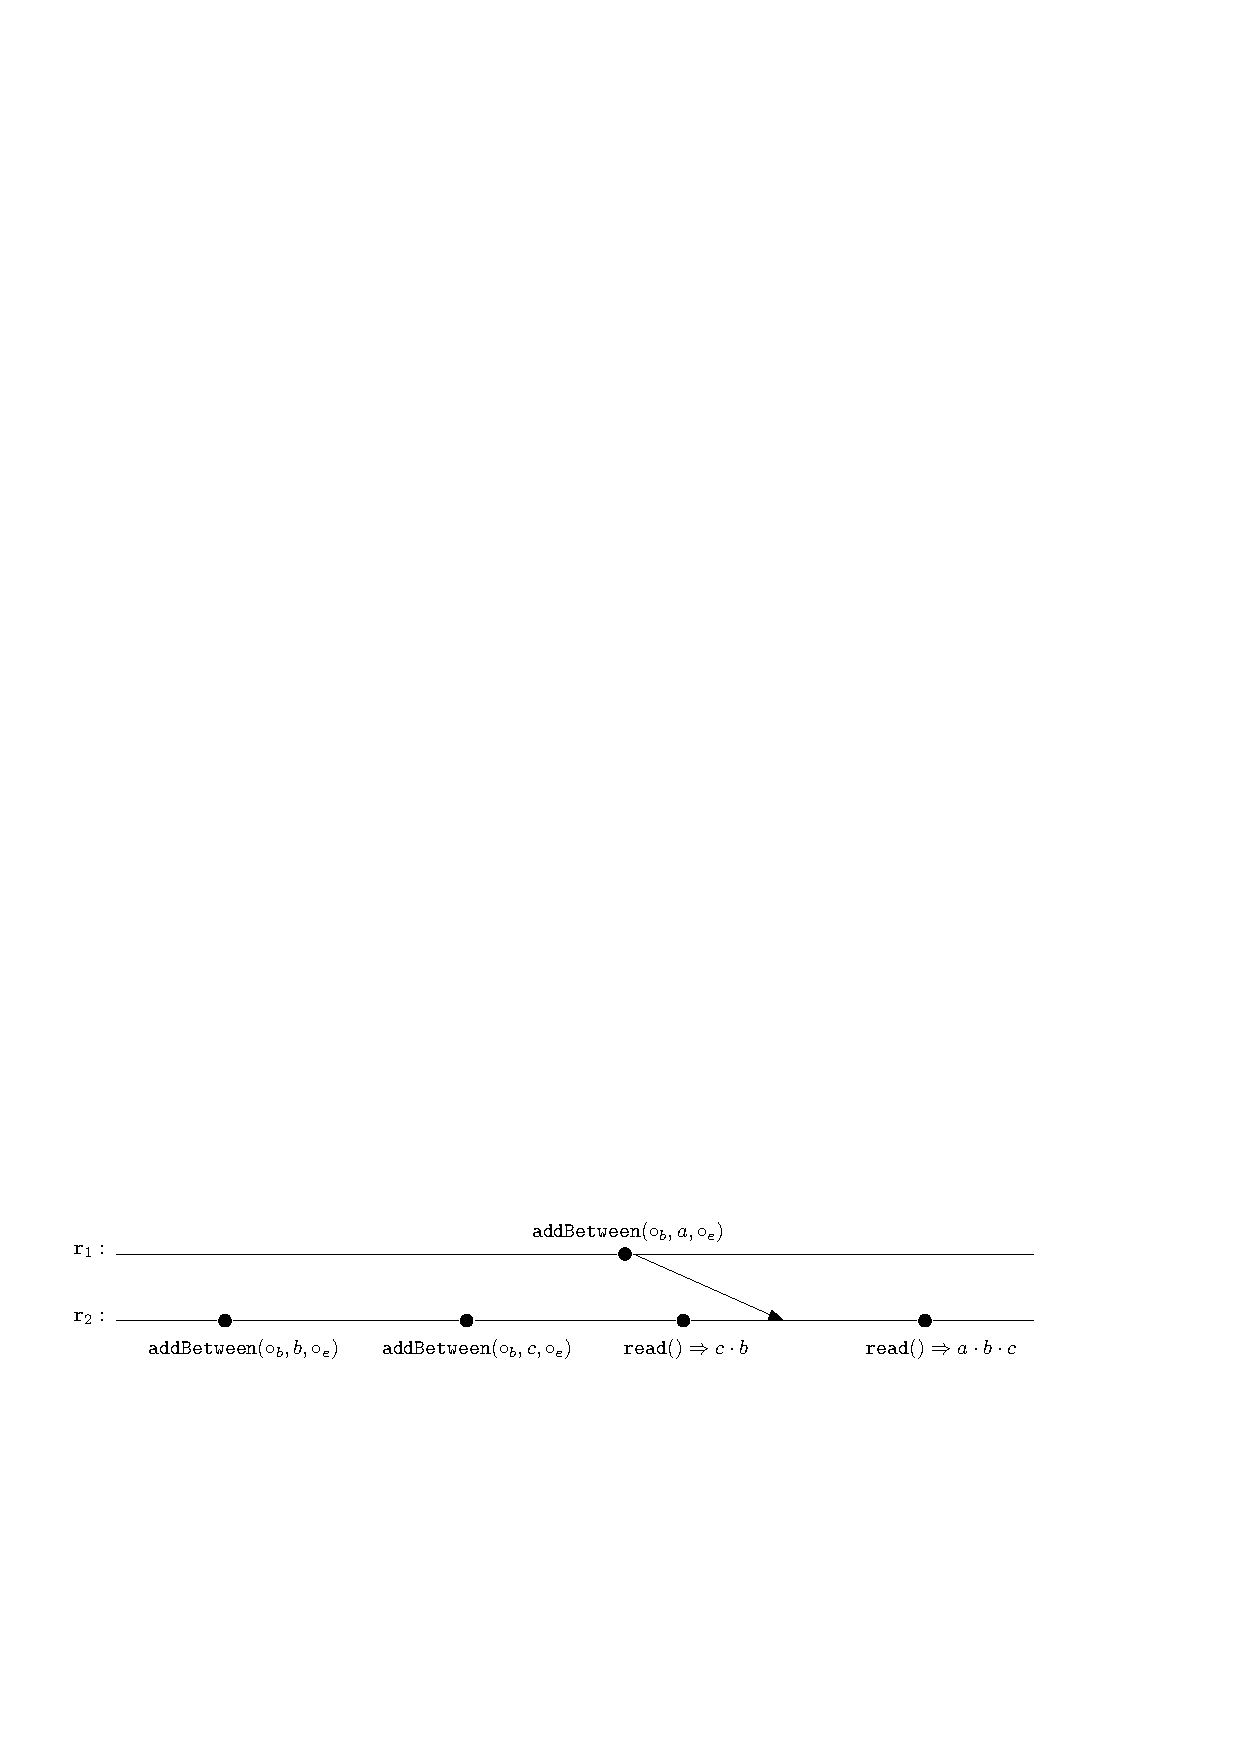
\includegraphics[width=0.85 \textwidth]{figures/ErrorExecutionofWooki.pdf}
\vspace{-10pt}
  \caption{A history w.r.t $\mathit{listBet}_s$ that should be excluded.}
  \label{fig:a wrong history w.r.t listbets}
\end{figure}

Given an execution $e$ of $\aobj$, we propose the following two property of $e$: Given local state $\sigma_1$ and $\sigma_2$ of $e$, if $\sigma_1$ (resp., $\sigma_2$) is obtained from the initial local state by applying a sequence $s_1$ of downstream (resp., a sequence $s_2$ of downstream).

\begin{itemize}
\setlength{\itemsep}{0.5pt}
\item[-] Convergence: if $s_1 \cap \updates = s_2 \cap \updates$, then $\sigma_1 = \sigma_2$.

\item[-] Consistent Conflict Resolution: if $s_1 \cap \updates$ is a sub-sequence of $s_2 \cap \updates$. Let $S$ be the set of downstream of update operations that are in $s_2$ and not in $s_1$, and let $s_3$ be a sequences of $S$ that is consistent with visibility relation. Then, we can obtain $\sigma_2$ from $\sigma_1$ by applying the downstream sequence $s_3$.
\end{itemize}

We say an execution $e$ is ready for downstream, if given a local state $\sigma$ of $e$ which is of replica $\arep$, we can safely apply all the downstream that are still not visible to replica $\arep$ in any order consistent with visibility relation.

Let us go back to \autoref{fig:a wrong history w.r.t listbets}. Let $\sigma_1$ be the local state of $\arep_2$ after we do $\alabelshort[{\tt addBetween}]{\circ_{begin},c,\circ_{end}}$, and let $\sigma_2$ be the local state of $\arep_2$ after we apply the downstream of $\alabelshort[{\tt addBetween}]{\circ_{begin},a,\circ_{end}}$.

$\alabelshort[{\tt addBetween}]{\circ_{begin},c,\circ_{end}}$

$\alabellong[{\tt read}]{}{c \cdot b}{}$,

The following lemma states that, once we prove ready for downstream and downstream of concurrent operations commute, we can obtain convergence and consistent conflict resolution, no matter whether the \Spec{} is deterministic or non-deterministic.

\begin{lemma}
\label{lemma:execution-order linearization ensures convergence and consistent conflict resolution}
If $\aobj$ is \crdtlinearizable{} w.r.t \Spec{} and each of its execution is ready for downstream.
execution-order linearizations

When doing $\alabelshort[{\tt integreteIns}]{c_p,c,c_n}$, for each $i$, $F[i],F[i+1]$ are degree-$d_{min}$-adjacent.
\end{lemma}

\begin {proof}
Obviously, $F[i],F[i+1]$ have degree $d_{min}$, and there is no W-character with degree $d_{min}$ and between $F[i]$ and $F[i+1]$ in $string_s$.

Since $d_{min}$ is the minimal degree of W-characters in $S'$, there does not exists W-character that is between $F[i]$ and $F[i+1]$ and will a degree smaller than $d_{min}$. This completes the proof of this lemma. $\qed$
\end {proof}






\subsection{\crdtlin{} with Non-Deterministic Sequential Specifications}
\label{subsec:appendix RA-linearizability with non-deterministic sequential specifications}

Recall that a sequential specification \Spec{} is deterministic, if for every label, the transition from a given initial state can produce at most one final state. Otherwise, we say that \Spec{} is non-deterministic.

Similarly as in Section \ref{subsec:definition of distributed linearizability}, let us provide the definition of \crdtlin{} with non-deterministic sequential specifications. For presentation reasons, we first consider the case where all the labels in the history are either queries or updates. We say a sequence $s$ is closed under a relation $R$, if when $a$ is in $s$ and $(a,b) \in R$, we have $b$ also in $s$.

\begin{definition}
\label{definition:ralinearizability1 with non-deterministic specifications}
A history $h = (\alabelset,\avisord)$ with $\alabelset\subseteq \queries\cup\updates$ is \crdtlinearizable{} w.r.t. a non-deterministic sequential specification \Spec{}, if there exists a specification sequence $(\alabelset, \aseqord) \in \Spec{}$, called the \emph{\crdtlinearization{}} of $h$, where we remark that the set of labels are identical, such that
\begin{enumerate}[(i)]
\item \aseqord{} is consistent with  \avisord{}, that is: $(\avisord \cup \aseqord)^{+}$ is acyclic,

\item the projection of $\aseqord$ to \emph{updates} is admitted by $\Spec$, i.e. $\aseqord\!\downarrow_{\updates} \in \Spec$,

\item There exists a function $\gconfres: \labels^* \rightarrow \abstates$ (Here the name $\gconfres$ is short for global conflict resolution). Given sequence $s \in \labels^*$, such that $s$ is consistent with $\avisord$ and closed under $\avisord^{-1}$, $\gconfres(s)$ is defined as follows: assume $\abstate_0$ is the initial abstract state of \Spec{},

$$ \gconfres(s)=\left\{
\begin{aligned}
an \ element \ of \ S &  & If \ S = \{ \abstate \vert \abstate_0 \xrightarrow{ \aseqord\!\downarrow_{s\cap \updates} }^* \abstate \} \neq \emptyset \\
undefined & & Otherwise
\end{aligned}
\right.
$$

%$\aseqord\!\downarrow_{s\cap \updates} \in \Spec$

Moreover, we require function $\gconfres$ to satisfy a property called $\mathsf{ConsistentChoice}$:

\begin{itemize}
\setlength{\itemsep}{0.5pt}
\item[-] $\mathsf{ConsistentChoice}$: Given two sub-sequences $s_1,s_2$, such that $s_1$ and $s_2$ are both consistent with $\avisord{}$, $s_1$ and $s_2$ are both closed under $\avisord{}^{-1}$, and $s_1$ is a sub-sequence of $s_2$. Then, $\gconfres(s_1) \xrightarrow{ s_2 - s_1 }^* \gconfres(s_2)$, where $s_2 - s_1$ denotes the sequences obtained from $s_2$ by removing elements of $s_1$.

%$\mathsf{ConsistentChoice}$: Given two sub-sequences $s_1,s_2$ of $\aseqord\!\downarrow_{\updates}$, if $s_2$ contains more operations than $s_1$, and both $\gconfres(s_1)$ and $\gconfres(s_2)$ are defined, then, $\gconfres(s_1) \xrightarrow{ s_2 - s_1 }^* \gconfres(s_2)$, where $s_2 - s_1$ denotes the sequences obtained from $s_2$ by removing elements of $s_1$.
\end{itemize}

\item for each query $\alabel_{\mathsf{qr}}\in \alabelset$, let $s = \avisord^{-1}(\alabel_{\mathsf{qr}})\cap \updates$. Then, we require that $\gconfres(s) \xrightarrow{ \alabel_{\mathsf{qr}} } \gconfres(s)$.
\end{enumerate}
In this case we say that $(\alabelset, \aseqord)$ is an \emph{\crdtlinearization{}} of $h$ w.r.t. $\Spec{}$.
\end{definition}

Let us explain Definition \ref{definition:ralinearizability1 with non-deterministic specifications}. Although $\Spec{}$ is non-deterministic, we use $\gconfres(s)$ to remember our choice for operation sequence $s$. Our definition need to concern two aspects:

\begin{itemize}
\setlength{\itemsep}{0.5pt}
\item[-] Convergence: To obtain $\gconfres(s)$ we only consider $\aseqord\!\downarrow_{s\cap \updates}$, which obviously implies convergence when we consider $\gconfres(s)$ and $\gconfres(s')$ and $s$ is a permutation of $s'$.

\item[-] Unique Choice in Specification: We should get rid of histories that have several operations that use ``Inconsistent non-deterministic choice''.

An example $h$ of such history is shown in \autoref{fig:a wrong history w.r.t listbets}. If only $\alabellong[{\tt read}]{}{c \cdot b}{}$ or $\alabellong[{\tt read}]{}{a \cdot b \cdot c}{}$ exists in $h$, then each of them is reasonable, since $\alabelshort[{\tt remove}]{a_2,a_1,a_3}$ puts $a_1$ in a random position between $a_2$ and $a_3$. However, $\alabellong[{\tt read}]{}{c \cdot b}{}$ represents that $c$ is put before $b$, while $\alabellong[{\tt read}]{}{a \cdot b \cdot c}{}$ represents that $b$ is before $c$. Therefore, we can not put these two $read$ operation in one history.

Since the set of operations visible to $\alabellong[{\tt read}]{}{c \cdot b}{}$ and the set of operations visible to $\alabellong[{\tt read}]{}{a \cdot b \cdot c}{}$ are different, our convergence requirement is not enough to rule them out. Instead, the $\mathsf{ConsistentChoice}$ condition is able to rule them out. $\mathsf{ConsistentChoice}$ essentially represents that, a ``bigger state'' follows the same choice in a ``smaller'' state.
\end{itemize}

\begin{figure}[t]
  \centering
  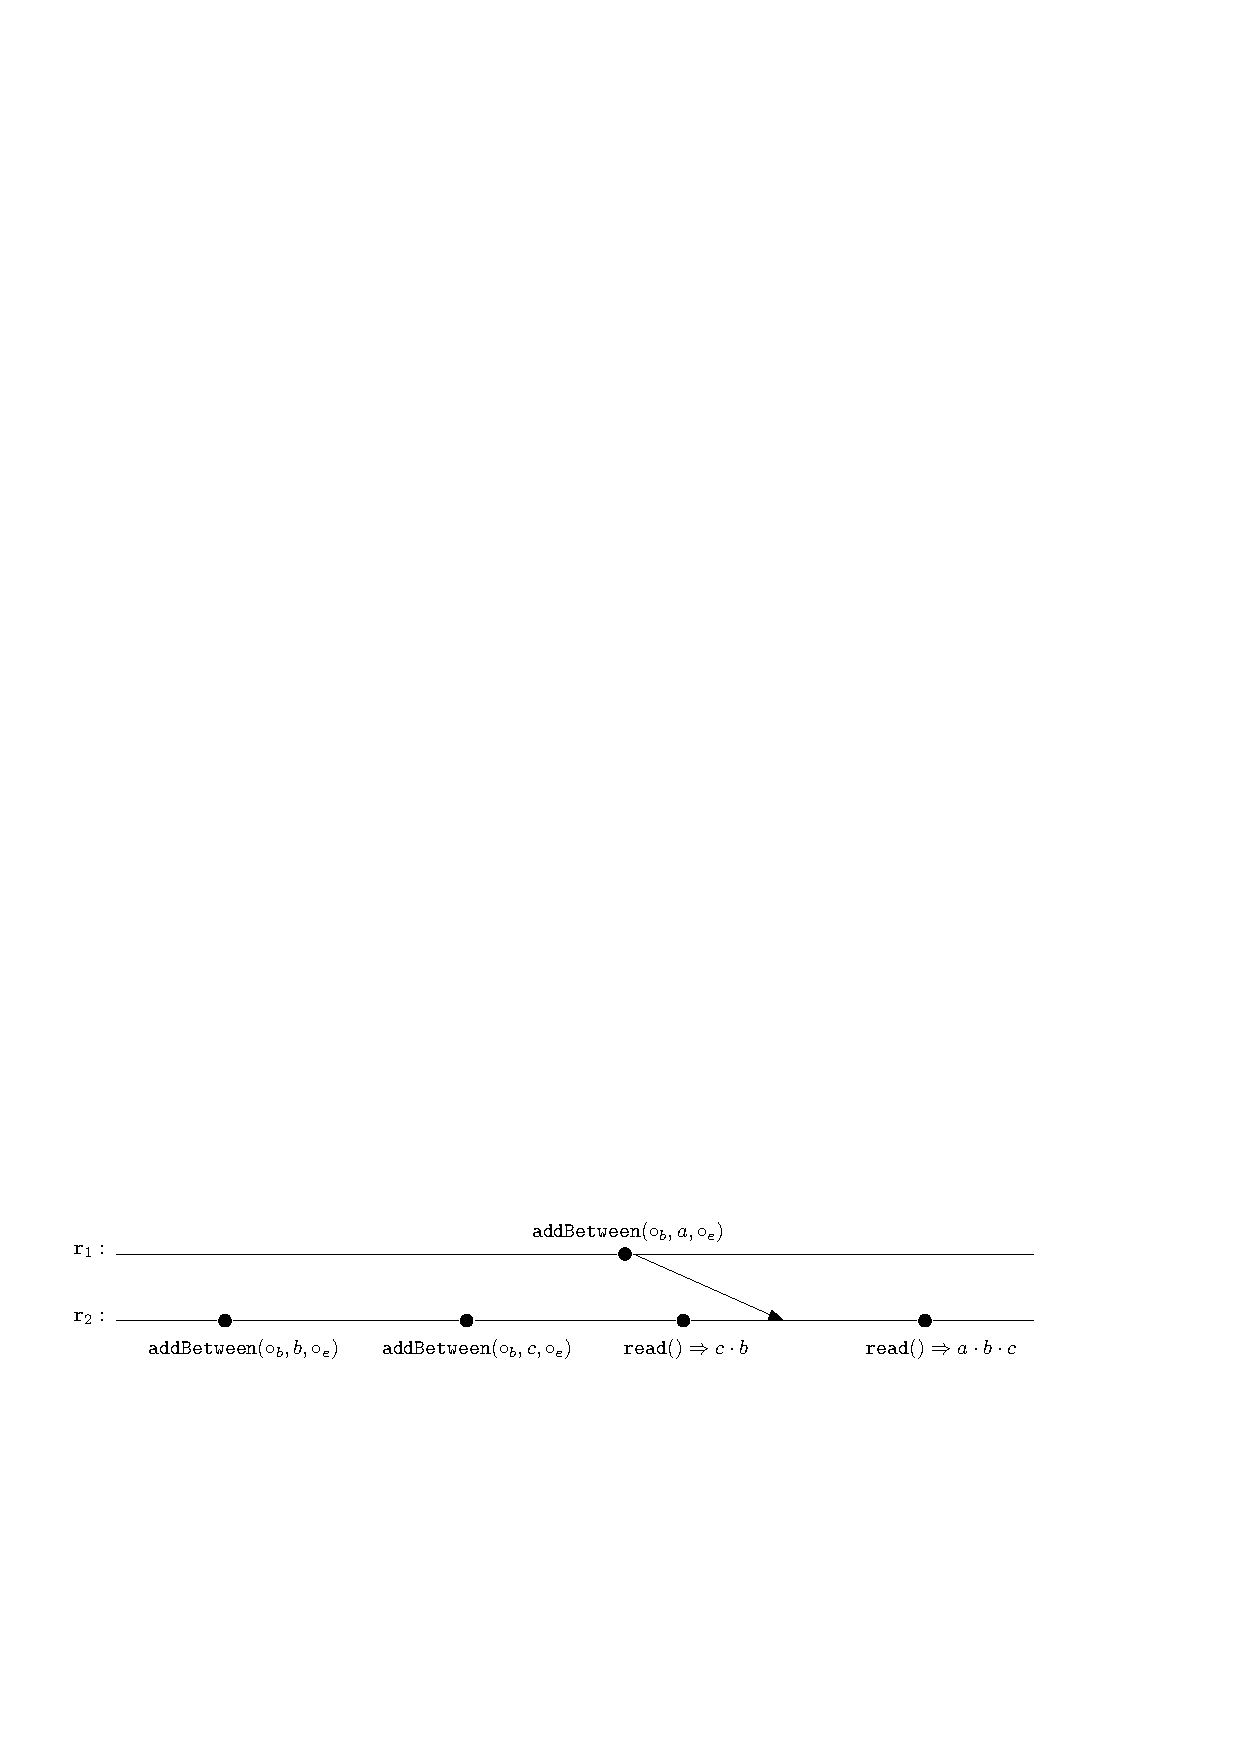
\includegraphics[width=0.85 \textwidth]{figures/ErrorExecutionofWooki.pdf}
\vspace{-10pt}
  \caption{A ``wrong'' history w.r.t $\mathit{listBet}_s$.}
  \label{fig:a wrong history w.r.t listbets}
\end{figure}


%Since the sequential specification is non-deterministic, for each operation sequence $s$, we fix $\gconfres(s)$ to be the consequence in sequential specification when applying update operations in $s$ according to \aseqord{} order from the initial abstract state $\abstate_0$ of sequential specification. The condition of $\gconfres(s_1) \xrightarrow{ s_2 - s_1 }^* \gconfres(s_2)$utf ensures that, the conflict resolution of bigger state $\gconfres(s_2)$ should also respect the conflict resolution of smaller state $\gconfres(s_1)$. Or we cam say, $\gconfres(s_1)$ is a ``sub-state'' of $\gconfres(s_2)$.

The case when histories include query-updates is similarly dealt with as Definition \ref{definition:distributed linearizability}. We do it by rewriting of the original history where each query-update is decomposed into a label representing the query part and another label representing the update part.

\begin{definition}[\CRDTLin{} with Non-Deterministic Sequential Specifications]
\label{definition:ralinearizability with non-deterministic sequential specifications and rewritting}
A history $h =(\alabelset,\avisord)$ is \crdtlinearizable{} w.r.t. a non-deterministic sequential specification \Spec{}, if there exists a query-update rewriting $\gamma$ such that $\gamma(h)$ is \crdtlinearizable{} w.r.t. \Spec{}.
\end{definition}

A set $H$ of histories is called \crdtlinearizable{} w.r.t a non-deterministic sequential specification $\Spec$ when each history $h\in H$ is \crdtlinearizable{} w.r.t. $\Spec$. A data type implementation is \crdtlinearizable{} w.r.t. a non-deterministic sequential specification $\Spec$ if for any object $\aobj$ of the data type, the set $\histories(\aobj)$ is linearizable w.r.t. $\Spec$.

Let us begin to consider convergence. Given a \crdtlinearizable{} history with two replicas $r_1,r_2$ see the same set of operations. According to Definition \ref{definition:ralinearizability1 with non-deterministic specifications} and Definition \ref{definition:ralinearizability with non-deterministic sequential specifications and rewritting}, to obtain $\gconfres(s)$, we only consider $\aseqord\!\downarrow_{s\cap \updates}$, which obviously implies convergence, as formalized in the following lemma.

\begin{lemma}
\label{lemma:distributed linarizability implies convergence for non-deterministic sequential specifications}
If a history $h$ is \crdtlinearizable{} w.r.t. a non-deterministic sequential specification \Spec, then $h$ is convergent.
\end{lemma}






\subsection{Proof Methodology for \crdtlin{} w.r.t Non-Deterministic Sequential Specifications}
\label{subsec:appendix proof methodology for RA-linearizability w.r.t non-deterministic sequential specifications}

In this subsection, we propose our methodology for proving \crdtlin{} w.r.t non-deterministic sequential specifications. Our methodology is similar for proving \crdtlin{} w.r.t deterministic sequential specifications in Section \ref{ssec:proof-methodology}.

%The similar points are as follows:

%\begin{itemize}
%\item[-] We still instrument the object semantics with an auxiliary variable $\alinord$ recording a linearization of the current history. %Only the execution of an \lstinline|atSource| portion of an operation engenders the extension of $\alinord$ by adding the current operation at some specific position. To guarantee that the linearization is consistent with the visibility relation, the operation must be inserted in the linearization after all the operations which are visible at the replica executing \lstinline|atSource|.

%\item[-] We still need to prove the property $\mathsf{ReplicaStates}$ and $\mathsf{\CRDTLinshort{}}$.

    %\begin{itemize}
    %\item[-] $\mathsf{ReplicaStates}$: requiring that for each replica $\arep$ with local configuration $(\alabelset,\astate)$, the state $\sigma$ is obtained by applying the downstreams of the operations in $\alabelset$ (that have been delivered to $\arep$) in the order defined by $\alinord$, and

    %\item[-] $\mathsf{\CRDTLinshort{}}$: requiring that the sequence $\alinord$ is an \crdtlinearization{} of the current history (w.r.t. $\Spec{}$).
    %\end{itemize}

%\item[-] We still rely on additional assertions describing the effect of each downstream.

%\item[-] We still need to prove $\mathsf{Refinement}$. The proof of $\mathsf{Refinement}$ still relies on a refinement mapping between replica states and states of the specification, denoted by $\refmap$.

    %\begin{itemize}
    %\item[-] $\mathsf{Refinement}$: each downstream produced by an update $\alabel$ and respectively, each query $\alabel$, is simulated by the application of $\alabel$ in the specification $\Spec$.
    %\end{itemize}
%\end{itemize}

Additionally, we need the following definitions:

\begin{itemize}
\setlength{\itemsep}{0.5pt}
\item[-] We introduce a function $\igconfres: \labels^* \rightarrow \states$ to explicitly record the consequence of applying downstream.

Given a sequence $s$ of downstream, such that $s$ is consistent with $\avisord$ and closed under $\avisord^{-1}$, $\igconfres(s)$ is the local state obtained by applying downstream of $s$ in the order of $s$.

\item[-] From $\igconfres(s)$, we generate a abstract state $\gconfres'(s)$. Latter we will prove that $\gconfres'$ satisfies the requirement of $\gconfres$.

    We use a refinement mapping $\refmap$ that maps $\igconfres(s)$ into $\gconfres'(s)$. %Or we can say, $\refmap{}(\igconfres(s)) = \gconfres(s)$.
\end{itemize}

%$\igconfres(s)$ may be undefined for some sequence $s$, for example, apply the downstream of $\alabelshort[{\tt remove}]{a}$ when no downstream of inserting $a$ has been applied.

Here the name $\igconfres$ is short for global conflict resolution in implementations.

Then, we need to prove the following properties:

\begin{itemize}
\setlength{\itemsep}{0.5pt}
\item[-] We prove that any two downstream that correspond to two ``concurrent'' operations commute.

\item[-] We prove $\mathsf{Refinement}$ holds between $\igconfres(s)$ and $\gconfres'(s)$ in a way as follows:

\begin{enumerate}
\item Given an update operation $\alabel$, if $s \cdot \alabel$ is consistent with $\avisord$ and closed under $\avisord^{-1}$, obviously $\igconfres(s \cdot \alabel)$ is obtained from $\igconfres(s)$ by applying the downstream of $\alabel$. Then, we require that $\gconfres'(s)\xRightarrow{\alabel}\gconfres'(s \cdot \alabel)$.

\item If a query $\alabel$ is applied on a state $\igconfres(s)$ or it is introduced by a rewriting of a query-update that executes \lstinline|atSource| on a state $\igconfres(s)$, then $\gconfres'(s)\xRightarrow{\alabel}\gconfres'(s)$.
\end{enumerate}
\end{itemize}

With above definitions and properties, our proof proceed as follows:

\noindent {\bf Prove correctness of $\gconfres'$:} We prove that $\gconfres'$ satisfies the requirement of $\gconfres$ as follows:

\begin{itemize}
\setlength{\itemsep}{0.5pt}
\item[-] Given sequences $s_1$ and $s_2$, such that both $s_1$ and $s_2$ are consistent with $\avisord$ and are closed under $\avisord^{-1}$, and $s_1$ is a permutation of $s_2$. Then, since any two downstream that correspond to two ``concurrent'' operations commute, we can see that $\igconfres(s_1)$ = $\igconfres(s_2)$. Since $\mathsf{Refinement}$ holds, we have transitions $\gconfres'(\epsilon)\xRightarrow{s_1}^*\gconfres'(s_1)$ and $\gconfres'(\epsilon)\xRightarrow{s_2}^*\gconfres'(s_2)$. Thus, $\gconfres'(s_1) = \gconfres'(s_2)$.

    Moreover, let $s_3$ be the projection of $\alinord$ into operations of $s_1$. Similarly, we can prove that $\gconfres'(s_1) = \gconfres'(s_3)$.

\item[-] $\mathsf{ConsistentChoice}$: Given $s_1$ and $s_2$, such that they are both consistent with $\avisord$ and closed under $\avisord^{-1}$, and $s_1$ is a sub-sequence of $s_2$. Obviously $s_1 \cdot (s_2 - s_1)$ is closed under $\avisord^{-1}$.

    We prove that $s_1 \cdot (s_2 - s_1)$ is consistent with $\avisord$ by contradiction. Assume that $s_1 \cdot (s_2 - s_1)$ is not consistent with $\avisord$. Since $s_1$ and $s_2$ are consistent with $\avisord$, this implies that, there exists $a,b$, such that, $a \in s_1$, $b \in s_2 - s_1$, and $(b,a) \in \avisord$. Or we can say, $(b,a) \in \avisord^{-1}$, $a \in s_1$, $b \notin s_1$. This contradicts the assumption that $s_1$ is closed under $\avisord^{-1}$. Therefore, $s_1 \cdot (s_2 - s_1)$ is consistent with $\avisord$.

    Since $s_2$ and $s_1 \cdot (s_2 - s_1)$ are consistent with $\avisord$ and closed under $\avisord^{-1}$, we know that there exists $\igconfres(s_2)$ and $\igconfres(s_1 \cdot (s_2 - s_1))$, and transitions from $\igconfres(\epsilon)$ to $\igconfres(s_2)$, and transitions from $\igconfres(\epsilon)$ to $\igconfres(s_1 \cdot (s_2 - s_1))$. By $\mathsf{Refinement}$, we know that there exist transitions $\gconfres'(\epsilon)\xRightarrow{s_2}^*\gconfres'(s_2)$ and transitions $\gconfres'(\epsilon)\xRightarrow{s_1}^*\gconfres'(s_1)\xRightarrow{s_2 - s_1}^*\gconfres'(s_1 \cdot (s_2 - s_1))$.

    Obviously, $s_2$ is a permutation of $s_1 \cdot (s_2 - s_1)$. As discussed above, we can see that $\gconfres'(s_2) = \gconfres'(s_1 \cdot (s_2 - s_1))$.
\end{itemize}

\noindent {\bf Prove $\mathsf{ReplicaStates}$:} $\mathsf{ReplicaStates}$ holds since any two downstream that correspond to two ``concurrent'' operations commute.

\noindent {\bf Prove $\mathsf{Refinement}$:} This is specific to implementations.

\noindent {\bf Prove Annotations:} If above proof relies on annotations of the downstream or local state, then we should also prove that the annotation of downstream holds for new downstream, and the annotation of local state holds for new local state.

\noindent {\bf Prove $\mathsf{\CRDTLinshort{}}$:} Similarly as in Section \ref{ssec:proof-methodology}, this is a consequence of $\mathsf{ReplicaStates}$, $\mathsf{Refinement}$, and the correctness of $\gconfres'$.


We have applied this methodology to Wooki and Tree-Doc. For Wooki and Tree-Doc, we use execution-order linearizations. The linearization $\alinord$ is defined by the order in which the \lstinline|atSource| procedures are executed.










\subsection{Proof of Wooki}
\label{subsec:proof of Wooki}




Then, let us prove that Wooki is \crdtlinearizable{} w.r.t $\mathit{listBet}_s$.

\begin{lemma}
\label{lemma:Wooki is correct}
Wooki is \crdtlinearizable{} w.r.t $\mathit{listBet}_s$.
\end{lemma}

\begin {proof}

We prove following the prove methodology of Section \ref{subsec:appendix proof methodology for RA-linearizability w.r.t non-deterministic sequential specifications}.

We define abstract state $\gconfres'(s)$ as follows: given a sequence $s$ of downstream, such that $s$ is consistent with $\avisord$ and closed under $\avisord^{-1}$, assume $\igconfres(s) = c_1 \dot \ldots \cdot c_n$, where for each $i$, $c_i = (id_i,v_i,degree_i,flag_i)$. Then, $\gconfres'(s) = (v_1 \cdot \ldots \cdot v_n,T)$, where $T = \{ v_i \vert flag_i = \mathit{false} \}$.

Then, let us prove the downstream of concurrent operations commute and the $\mathsf{Refinement}$ property,

\begin{itemize}
\setlength{\itemsep}{0.5pt}
\item[-] By Lemma \ref{lemma:in Wooki algorithm, two downstreams of two addBetween operations commute}, we can see that the downstream of concurrent {\tt addBetween} operations commute. According to Wooki algorithm, it is easy to see that the downstream of concurrent {\tt remove} operations commute, since they both put some value into tombstone; A {\tt addBetween} and a {\tt remove} downstream commute when they are concurrent because in this case, the W-character removed by {\tt remove} are different from the pair added by the {\tt addBetween}.
\item[-] Let us prove $\mathsf{Refinement}$ holds between $\igconfres(s)$ and $\gconfres'(s)$ as follows:

    \begin{itemize}
    \setlength{\itemsep}{0.5pt}
    \item[-] Given an operation $\alabel = \alabelshort[{\tt addBetween}]{a,b,c}$, assume that $s \cdot \alabel$ is consistent with $\avisord$ and closed under $\avisord^{-1}$. We need to prove that $\gconfres'(s)\xRightarrow{\alabel}\gconfres'(s \cdot \alabel)$.

        Assume that $\igconfres(s)=str_1$, and $\igconfres(s')=str_2$. We can see that there exists W-character $c_a = (\_,a,\_,\_)$ and $c_c = (\_,c,\_,\_)$ in $str_1$, such that $c_a$ is before $c_c$ in $str_1$, there is no W-character of value $b$ in $str_1$, and $str_2$ is obtained from $str_1$ by inserting a W-character $c_b = (\_,b,\_,\mathit{true})$ at some position between $c_a$ and $c_c$. Then, it is easy to see that $\gconfres'(s)\xRightarrow{\alabel}\gconfres'(s \cdot \alabel)$.

    \item[-] Given an operation $\alabel = \alabelshort[{\tt remove}]{b}$, assume that $s \cdot \alabel$ is consistent with $\avisord$ and closed under $\avisord^{-1}$. We need to prove that $\gconfres'(s)\xRightarrow{\alabel}\gconfres'(s \cdot \alabel)$.

        Assume that $\igconfres(s)=str_1$, and $\igconfres(s')=str_2$. We can see that there exists W-character $c_b = (\_,b,\_,\_)$ in $str_1$, and $str_2$ is obtained from $str_1$ by setting the flag of $c_b$ into $\mathit{false}$. Then, it is easy to see that $\gconfres'(s)\xRightarrow{\alabel}\gconfres'(s \cdot \alabel)$.

    \item[-] Given an operation $\alabel = \alabellong[{\tt read}]{}{s_1}{}$, assume that $s \cdot \alabel$ is consistent with $\avisord$ and closed under $\avisord^{-1}$. Assume that $\alabel$ is applied on the state $\igconfres(s)$. We need to prove that $\gconfres'(s)\xRightarrow{\alabel}\gconfres'(s)$.

        Assume that $\igconfres(s)=c_1 \cdot \ldots \cdot c_n$, where for each $i$, $c_i = (id_i,v_i,degree_i,flag_i)$. Then, $s_1$ is obtained from $v_1 \cdot \ldots \cdot v_n$ by removing values with flag $\mathit{false}$. Then, it is easy to see that $\gconfres'(s)\xRightarrow{\alabel}\gconfres'(s)$.
    \end{itemize}

\end{itemize}

Then, our proof proceeds as follows:

\begin{itemize}
\setlength{\itemsep}{0.5pt}
\item[-] {\bf Prove correctness of $\gconfres'$:} With above properties, as discussed in Section \ref{subsec:appendix proof methodology for RA-linearizability w.r.t non-deterministic sequential specifications}, we can prove that $\gconfres'$ satisfies the requirement of $\gconfres$ in Definition \ref{definition:ralinearizability1 with non-deterministic specifications}.

\item[-] {\bf Prove $\mathsf{ReplicaStates}$:} Since every operation is appended to the linearization when it executes {\tt atSource} it clearly follows, the linearization order is consistent with visibility order. Then, by the {\textred{causal delivery}} assumption, the order in which downstream are applied at a given replica is also consistent with the visibility order. Let $\alinord_1$ be the projection of linearization order into labels applied in a replica $\arep$, and $\alinord_2$ be the order of labels applied in replica $\arep$. By Lemma \ref{lemma:given two sequence consistent with visibility order, one can be obtained from the other}, $\alinord_2$ can be obtained from $\alinord_1$ by several time of swapping adjacent pair of concurrent operations. This holds, since we have already prove that, the downstream of concurrent operations commute.

\item[-] {\bf Prove $\mathsf{\CRDTLinshort{}}$:} Finally, we describe the proof of the fact that $\mathsf{\CRDTLinshort{}}$ is an inductive invariant. As already mentioned, appending operations to the linearization when they execute \lstinline|atSource| clearly implies that $\alinord$ is consistent with the visibility. Next, the projection of $\alinord$ on the updates is obviously admitted by the specification (the updates are always enabled from the point of view of the specification).
We also have to argue that for each query $\alabel_{\mathsf{qr}} = \alabellongind[read]{}{s_1}{}$, the sequence $\alinord'\cdot \alabel_{\mathsf{qr}}$ where $\alinord'$ is the projection of $\alinord$ on the set of updates
visible to $\alabel_{\mathsf{qr}}$ is admitted by the specification. First, by $\mathsf{ReplicaStates}$, the state $\sigma$ of the replica where $\alabel_{\mathsf{qr}}$ is applied is obtained by applying the downstream of the operations visible to $\alabel_{\mathsf{qr}}$ in the linearization order. Then, by $\mathsf{Refinement}$, every downstream is simulated by the corresponding operation in the context of the specification. This implies that $\gconfres'(\epsilon)\xRightarrow{\alinord'}^*\gconfres'(\alinord')$. The query $\alabel_{\mathsf{qr}}$ is also simulated by the same operation in the context of the specification, which implies that $\gconfres'(\alinord')\xRightarrow{\alabel_{\mathsf{qr}}}\gconfres'(\alinord')$. These two facts imply that $\gconfres'(\epsilon)\xRightarrow{\alinord'\cdot \alabel_{\mathsf{qr}}}^*\gconfres'(\alinord')$ which means that $\alinord'\cdot \alabel_{\mathsf{qr}}$ is admitted by the specification.
\end{itemize}

This completes the proof of this lemma. $\qed$
\end {proof}
}































\forget
{
\section{\crdtlin{} with Non-Deterministic Sequential Specifications and Its Proof}
\label{sec:appendix RA-linearizability with non-deterministic sequential specifications and its proof}



\subsection{\crdtlin{} with Non-Deterministic Sequential Specifications}
\label{subsec:appendix RA-linearizability with non-deterministic sequential specifications}

Recall that a sequential specification \Spec{} is deterministic, if for every label, the transition from a given initial state can produce at most one final state. Otherwise, we say that \Spec{} is non-deterministic.

Similarly as in Section \ref{subsec:definition of distributed linearizability}, let us provide the definition of \crdtlin{} with non-deterministic sequential specifications. For presentation reasons, we first consider the case where all the labels in the history are either queries or updates. We say a sequence $s$ is closed under a relation $R$, if when $a$ is in $s$ and $(a,b) \in R$, we have $b$ also in $s$.

\begin{definition}
\label{definition:ralinearizability1 with non-deterministic specifications}
A history $h = (\alabelset,\avisord)$ with $\alabelset\subseteq \queries\cup\updates$ is \crdtlinearizable{} w.r.t. a non-deterministic sequential specification \Spec{}, if there exists a specification sequence $(\alabelset, \aseqord) \in \Spec{}$, called the \emph{\crdtlinearization{}} of $h$, where we remark that the set of labels are identical, such that
\begin{enumerate}[(i)]
\item \aseqord{} is consistent with  \avisord{}, that is: $(\avisord \cup \aseqord)^{+}$ is acyclic,

\item the projection of $\aseqord$ to \emph{updates} is admitted by $\Spec$, i.e. $\aseqord\!\downarrow_{\updates} \in \Spec$,

\item There exists a function $\gconfres: \labels^* \rightarrow \abstates$ (Here the name $\gconfres$ is short for global conflict resolution). Given sequence $s \in \labels^*$, such that $s$ is consistent with $\avisord$ and closed under $\avisord^{-1}$, $\gconfres(s)$ is defined as follows: assume $\abstate_0$ is the initial abstract state of \Spec{},

$$ \gconfres(s)=\left\{
\begin{aligned}
an \ element \ of \ S &  & If \ S = \{ \abstate \vert \abstate_0 \xrightarrow{ \aseqord\!\downarrow_{s\cap \updates} }^* \abstate \} \neq \emptyset \\
undefined & & Otherwise
\end{aligned}
\right.
$$

%$\aseqord\!\downarrow_{s\cap \updates} \in \Spec$

Moreover, we require function $\gconfres$ to satisfy a property called $\mathsf{ConsistentChoice}$:

\begin{itemize}
\setlength{\itemsep}{0.5pt}
\item[-] $\mathsf{ConsistentChoice}$: Given two sub-sequences $s_1,s_2$, such that $s_1$ and $s_2$ are both consistent with $\avisord{}$, $s_1$ and $s_2$ are both closed under $\avisord{}^{-1}$, and $s_1$ is a sub-sequence of $s_2$. Then, $\gconfres(s_1) \xrightarrow{ s_2 - s_1 }^* \gconfres(s_2)$, where $s_2 - s_1$ denotes the sequences obtained from $s_2$ by removing elements of $s_1$.

%$\mathsf{ConsistentChoice}$: Given two sub-sequences $s_1,s_2$ of $\aseqord\!\downarrow_{\updates}$, if $s_2$ contains more operations than $s_1$, and both $\gconfres(s_1)$ and $\gconfres(s_2)$ are defined, then, $\gconfres(s_1) \xrightarrow{ s_2 - s_1 }^* \gconfres(s_2)$, where $s_2 - s_1$ denotes the sequences obtained from $s_2$ by removing elements of $s_1$.
\end{itemize}

\item for each query $\alabel_{\mathsf{qr}}\in \alabelset$, let $s = \avisord^{-1}(\alabel_{\mathsf{qr}})\cap \updates$. Then, we require that $\gconfres(s) \xrightarrow{ \alabel_{\mathsf{qr}} } \gconfres(s)$.
\end{enumerate}
In this case we say that $(\alabelset, \aseqord)$ is an \emph{\crdtlinearization{}} of $h$ w.r.t. $\Spec{}$.
\end{definition}

Let us explain Definition \ref{definition:ralinearizability1 with non-deterministic specifications}. Although $\Spec{}$ is non-deterministic, we use $\gconfres(s)$ to remember our choice for operation sequence $s$. Our definition need to concern two aspects:

\begin{itemize}
\setlength{\itemsep}{0.5pt}
\item[-] Convergence: To obtain $\gconfres(s)$ we only consider $\aseqord\!\downarrow_{s\cap \updates}$, which obviously implies convergence when we consider $\gconfres(s)$ and $\gconfres(s')$ and $s$ is a permutation of $s'$.

\item[-] Unique Choice in Specification: We should get rid of histories that have several operations that use ``Inconsistent non-deterministic choice''.

An example $h$ of such history is shown in \autoref{fig:a wrong history w.r.t listbets}. If only $\alabellong[{\tt read}]{}{c \cdot b}{}$ or $\alabellong[{\tt read}]{}{a \cdot b \cdot c}{}$ exists in $h$, then each of them is reasonable, since $\alabelshort[{\tt remove}]{a_2,a_1,a_3}$ puts $a_1$ in a random position between $a_2$ and $a_3$. However, $\alabellong[{\tt read}]{}{c \cdot b}{}$ represents that $c$ is put before $b$, while $\alabellong[{\tt read}]{}{a \cdot b \cdot c}{}$ represents that $b$ is before $c$. Therefore, we can not put these two $read$ operation in one history.

Since the set of operations visible to $\alabellong[{\tt read}]{}{c \cdot b}{}$ and the set of operations visible to $\alabellong[{\tt read}]{}{a \cdot b \cdot c}{}$ are different, our convergence requirement is not enough to rule them out. Instead, the $\mathsf{ConsistentChoice}$ condition is able to rule them out. $\mathsf{ConsistentChoice}$ essentially represents that, a ``bigger state'' follows the same choice in a ``smaller'' state.
\end{itemize}

\begin{figure}[t]
  \centering
  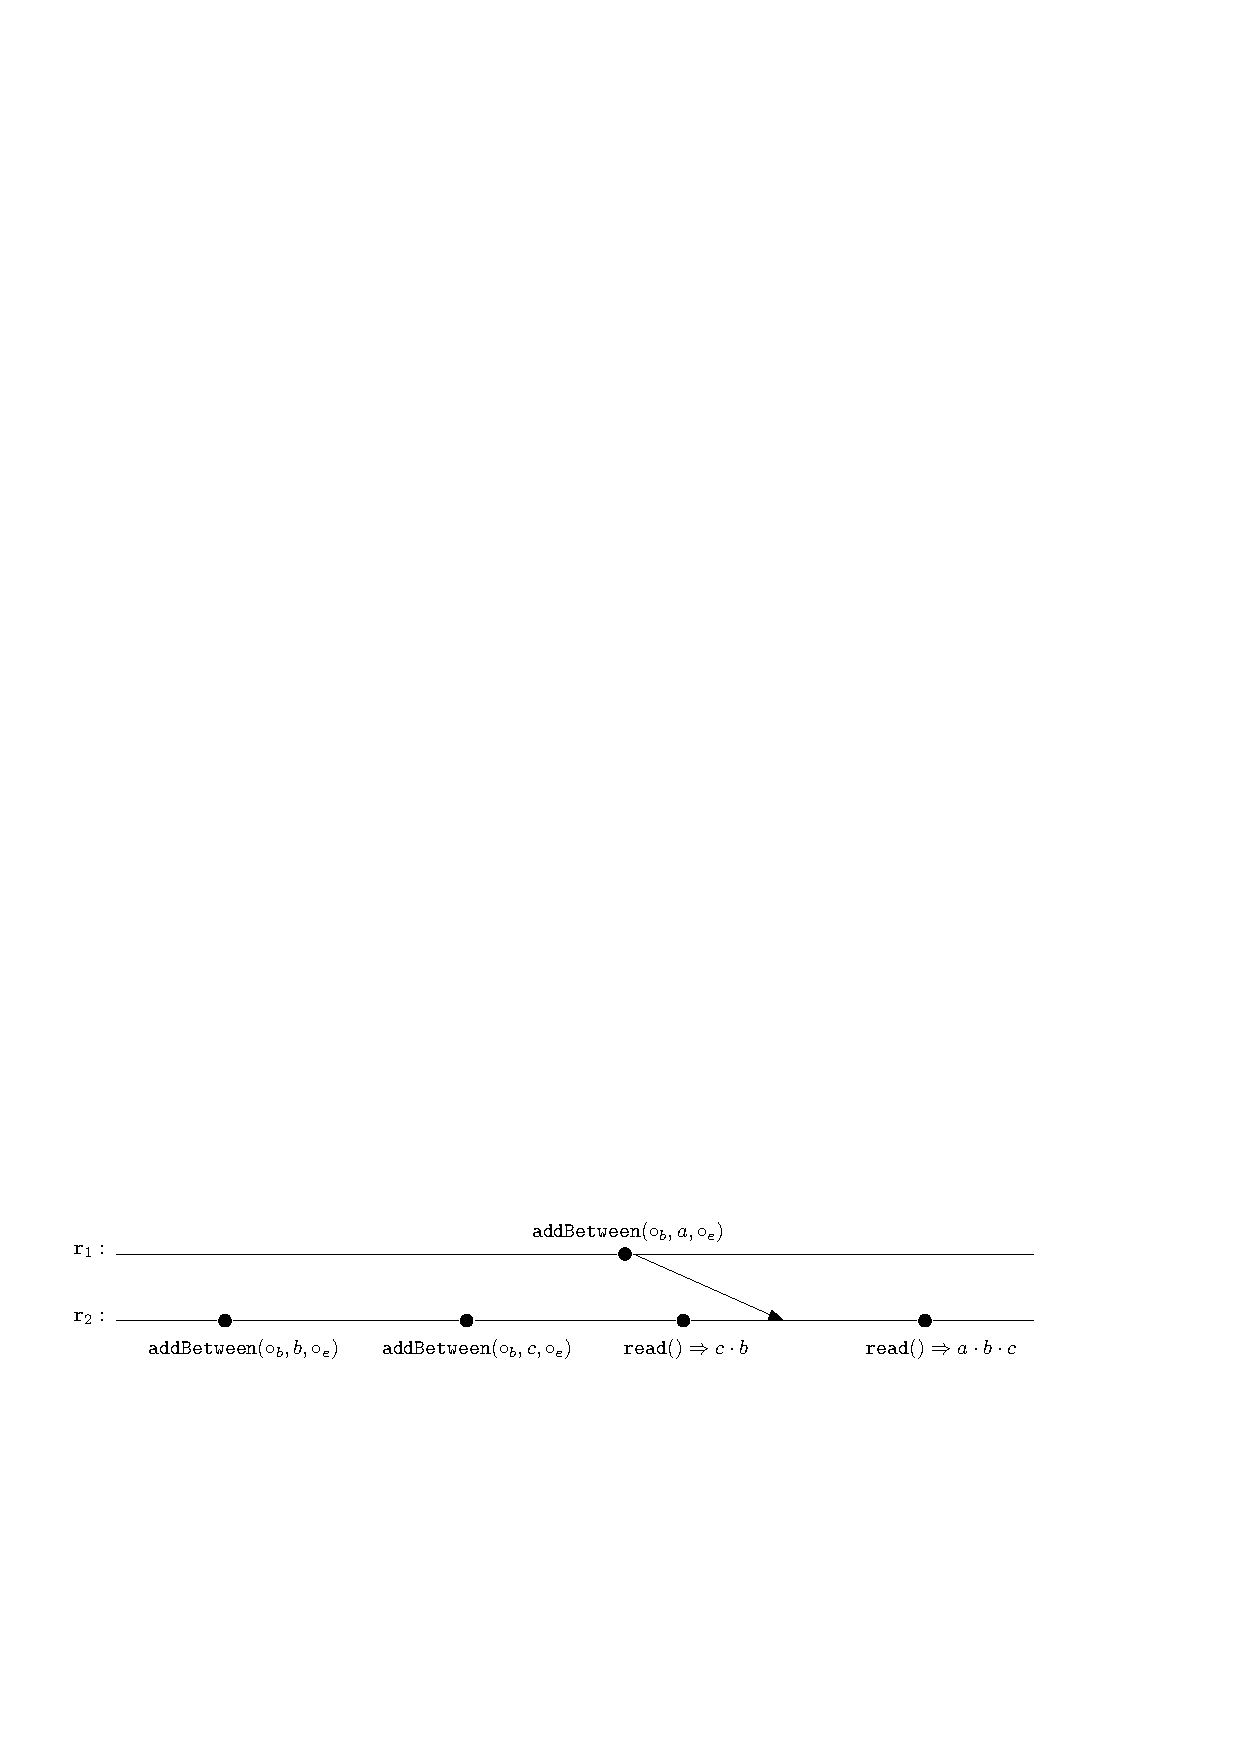
\includegraphics[width=0.85 \textwidth]{figures/ErrorExecutionofWooki.pdf}
\vspace{-10pt}
  \caption{A ``wrong'' history w.r.t $\mathit{listBet}_s$.}
  \label{fig:a wrong history w.r.t listbets}
\end{figure}


%Since the sequential specification is non-deterministic, for each operation sequence $s$, we fix $\gconfres(s)$ to be the consequence in sequential specification when applying update operations in $s$ according to \aseqord{} order from the initial abstract state $\abstate_0$ of sequential specification. The condition of $\gconfres(s_1) \xrightarrow{ s_2 - s_1 }^* \gconfres(s_2)$utf ensures that, the conflict resolution of bigger state $\gconfres(s_2)$ should also respect the conflict resolution of smaller state $\gconfres(s_1)$. Or we cam say, $\gconfres(s_1)$ is a ``sub-state'' of $\gconfres(s_2)$.

The case when histories include query-updates is similarly dealt with as Definition \ref{definition:distributed linearizability}. We do it by rewriting of the original history where each query-update is decomposed into a label representing the query part and another label representing the update part.

\begin{definition}[\CRDTLin{} with Non-Deterministic Sequential Specifications]
\label{definition:ralinearizability with non-deterministic sequential specifications and rewritting}
A history $h =(\alabelset,\avisord)$ is \crdtlinearizable{} w.r.t. a non-deterministic sequential specification \Spec{}, if there exists a query-update rewriting $\gamma$ such that $\gamma(h)$ is \crdtlinearizable{} w.r.t. \Spec{}.
\end{definition}

A set $H$ of histories is called \crdtlinearizable{} w.r.t a non-deterministic sequential specification $\Spec$ when each history $h\in H$ is \crdtlinearizable{} w.r.t. $\Spec$. A data type implementation is \crdtlinearizable{} w.r.t. a non-deterministic sequential specification $\Spec$ if for any object $\aobj$ of the data type, the set $\histories(\aobj)$ is linearizable w.r.t. $\Spec$.

Let us begin to consider convergence. Given a \crdtlinearizable{} history with two replicas $r_1,r_2$ see the same set of operations. According to Definition \ref{definition:ralinearizability1 with non-deterministic specifications} and Definition \ref{definition:ralinearizability with non-deterministic sequential specifications and rewritting}, to obtain $\gconfres(s)$, we only consider $\aseqord\!\downarrow_{s\cap \updates}$, which obviously implies convergence, as formalized in the following lemma.

\begin{lemma}
\label{lemma:distributed linarizability implies convergence for non-deterministic sequential specifications}
If a history $h$ is \crdtlinearizable{} w.r.t. a non-deterministic sequential specification \Spec, then $h$ is convergent.
\end{lemma}






\subsection{Proof Methodology for \crdtlin{} w.r.t Non-Deterministic Sequential Specifications}
\label{subsec:appendix proof methodology for RA-linearizability w.r.t non-deterministic sequential specifications}

In this subsection, we propose our methodology for proving \crdtlin{} w.r.t non-deterministic sequential specifications. Our methodology is similar for proving \crdtlin{} w.r.t deterministic sequential specifications in Section \ref{ssec:proof-methodology}.

%The similar points are as follows:

%\begin{itemize}
%\item[-] We still instrument the object semantics with an auxiliary variable $\alinord$ recording a linearization of the current history. %Only the execution of an \lstinline|atSource| portion of an operation engenders the extension of $\alinord$ by adding the current operation at some specific position. To guarantee that the linearization is consistent with the visibility relation, the operation must be inserted in the linearization after all the operations which are visible at the replica executing \lstinline|atSource|.

%\item[-] We still need to prove the property $\mathsf{ReplicaStates}$ and $\mathsf{\CRDTLinshort{}}$.

    %\begin{itemize}
    %\item[-] $\mathsf{ReplicaStates}$: requiring that for each replica $\arep$ with local configuration $(\alabelset,\astate)$, the state $\sigma$ is obtained by applying the downstreams of the operations in $\alabelset$ (that have been delivered to $\arep$) in the order defined by $\alinord$, and

    %\item[-] $\mathsf{\CRDTLinshort{}}$: requiring that the sequence $\alinord$ is an \crdtlinearization{} of the current history (w.r.t. $\Spec{}$).
    %\end{itemize}

%\item[-] We still rely on additional assertions describing the effect of each downstream.

%\item[-] We still need to prove $\mathsf{Refinement}$. The proof of $\mathsf{Refinement}$ still relies on a refinement mapping between replica states and states of the specification, denoted by $\refmap$.

    %\begin{itemize}
    %\item[-] $\mathsf{Refinement}$: each downstream produced by an update $\alabel$ and respectively, each query $\alabel$, is simulated by the application of $\alabel$ in the specification $\Spec$.
    %\end{itemize}
%\end{itemize}

Additionally, we need the following definitions:

\begin{itemize}
\setlength{\itemsep}{0.5pt}
\item[-] We introduce a function $\igconfres: \labels^* \rightarrow \states$ to explicitly record the consequence of applying downstream.

Given a sequence $s$ of downstream, such that $s$ is consistent with $\avisord$ and closed under $\avisord^{-1}$, $\igconfres(s)$ is the local state obtained by applying downstream of $s$ in the order of $s$.

\item[-] From $\igconfres(s)$, we generate a abstract state $\gconfres'(s)$. Latter we will prove that $\gconfres'$ satisfies the requirement of $\gconfres$.

    We use a refinement mapping $\refmap$ that maps $\igconfres(s)$ into $\gconfres'(s)$. %Or we can say, $\refmap{}(\igconfres(s)) = \gconfres(s)$.
\end{itemize}

%$\igconfres(s)$ may be undefined for some sequence $s$, for example, apply the downstream of $\alabelshort[{\tt remove}]{a}$ when no downstream of inserting $a$ has been applied.

Here the name $\igconfres$ is short for global conflict resolution in implementations.

Then, we need to prove the following properties:

\begin{itemize}
\setlength{\itemsep}{0.5pt}
\item[-] We prove that any two downstream that correspond to two ``concurrent'' operations commute.

\item[-] We prove $\mathsf{Refinement}$ holds between $\igconfres(s)$ and $\gconfres'(s)$ in a way as follows:

\begin{enumerate}
\item Given an update operation $\alabel$, if $s \cdot \alabel$ is consistent with $\avisord$ and closed under $\avisord^{-1}$, obviously $\igconfres(s \cdot \alabel)$ is obtained from $\igconfres(s)$ by applying the downstream of $\alabel$. Then, we require that $\gconfres'(s)\xRightarrow{\alabel}\gconfres'(s \cdot \alabel)$.

\item If a query $\alabel$ is applied on a state $\igconfres(s)$ or it is introduced by a rewriting of a query-update that executes \lstinline|atSource| on a state $\igconfres(s)$, then $\gconfres'(s)\xRightarrow{\alabel}\gconfres'(s)$.
\end{enumerate}
\end{itemize}

With above definitions and properties, our proof proceed as follows:

\noindent {\bf Prove correctness of $\gconfres'$:} We prove that $\gconfres'$ satisfies the requirement of $\gconfres$ as follows:

\begin{itemize}
\setlength{\itemsep}{0.5pt}
\item[-] Given sequences $s_1$ and $s_2$, such that both $s_1$ and $s_2$ are consistent with $\avisord$ and are closed under $\avisord^{-1}$, and $s_1$ is a permutation of $s_2$. Then, since any two downstream that correspond to two ``concurrent'' operations commute, we can see that $\igconfres(s_1)$ = $\igconfres(s_2)$. Since $\mathsf{Refinement}$ holds, we have transitions $\gconfres'(\epsilon)\xRightarrow{s_1}^*\gconfres'(s_1)$ and $\gconfres'(\epsilon)\xRightarrow{s_2}^*\gconfres'(s_2)$. Thus, $\gconfres'(s_1) = \gconfres'(s_2)$.

    Moreover, let $s_3$ be the projection of $\alinord$ into operations of $s_1$. Similarly, we can prove that $\gconfres'(s_1) = \gconfres'(s_3)$.

\item[-] $\mathsf{ConsistentChoice}$: Given $s_1$ and $s_2$, such that they are both consistent with $\avisord$ and closed under $\avisord^{-1}$, and $s_1$ is a sub-sequence of $s_2$. Obviously $s_1 \cdot (s_2 - s_1)$ is closed under $\avisord^{-1}$.

    We prove that $s_1 \cdot (s_2 - s_1)$ is consistent with $\avisord$ by contradiction. Assume that $s_1 \cdot (s_2 - s_1)$ is not consistent with $\avisord$. Since $s_1$ and $s_2$ are consistent with $\avisord$, this implies that, there exists $a,b$, such that, $a \in s_1$, $b \in s_2 - s_1$, and $(b,a) \in \avisord$. Or we can say, $(b,a) \in \avisord^{-1}$, $a \in s_1$, $b \notin s_1$. This contradicts the assumption that $s_1$ is closed under $\avisord^{-1}$. Therefore, $s_1 \cdot (s_2 - s_1)$ is consistent with $\avisord$.

    Since $s_2$ and $s_1 \cdot (s_2 - s_1)$ are consistent with $\avisord$ and closed under $\avisord^{-1}$, we know that there exists $\igconfres(s_2)$ and $\igconfres(s_1 \cdot (s_2 - s_1))$, and transitions from $\igconfres(\epsilon)$ to $\igconfres(s_2)$, and transitions from $\igconfres(\epsilon)$ to $\igconfres(s_1 \cdot (s_2 - s_1))$. By $\mathsf{Refinement}$, we know that there exist transitions $\gconfres'(\epsilon)\xRightarrow{s_2}^*\gconfres'(s_2)$ and transitions $\gconfres'(\epsilon)\xRightarrow{s_1}^*\gconfres'(s_1)\xRightarrow{s_2 - s_1}^*\gconfres'(s_1 \cdot (s_2 - s_1))$.

    Obviously, $s_2$ is a permutation of $s_1 \cdot (s_2 - s_1)$. As discussed above, we can see that $\gconfres'(s_2) = \gconfres'(s_1 \cdot (s_2 - s_1))$.
\end{itemize}

\noindent {\bf Prove $\mathsf{ReplicaStates}$:} $\mathsf{ReplicaStates}$ holds since any two downstream that correspond to two ``concurrent'' operations commute.

\noindent {\bf Prove $\mathsf{Refinement}$:} This is specific to implementations.

\noindent {\bf Prove Annotations:} If above proof relies on annotations of the downstream or local state, then we should also prove that the annotation of downstream holds for new downstream, and the annotation of local state holds for new local state.

\noindent {\bf Prove $\mathsf{\CRDTLinshort{}}$:} Similarly as in Section \ref{ssec:proof-methodology}, this is a consequence of $\mathsf{ReplicaStates}$, $\mathsf{Refinement}$, and the correctness of $\gconfres'$.


We have applied this methodology to Wooki and Tree-Doc. For Wooki and Tree-Doc, we use execution-order linearizations. The linearization $\alinord$ is defined by the order in which the \lstinline|atSource| procedures are executed.










\subsection{Proof of Wooki}
\label{subsec:proof of Wooki}




Then, let us prove that Wooki is \crdtlinearizable{} w.r.t $\mathit{listBet}_s$.

\begin{lemma}
\label{lemma:Wooki is correct}
Wooki is \crdtlinearizable{} w.r.t $\mathit{listBet}_s$.
\end{lemma}

\begin {proof}

We prove following the prove methodology of Section \ref{subsec:appendix proof methodology for RA-linearizability w.r.t non-deterministic sequential specifications}.

We define abstract state $\gconfres'(s)$ as follows: given a sequence $s$ of downstream, such that $s$ is consistent with $\avisord$ and closed under $\avisord^{-1}$, assume $\igconfres(s) = c_1 \dot \ldots \cdot c_n$, where for each $i$, $c_i = (id_i,v_i,degree_i,flag_i)$. Then, $\gconfres'(s) = (v_1 \cdot \ldots \cdot v_n,T)$, where $T = \{ v_i \vert flag_i = \mathit{false} \}$.

Then, let us prove the downstream of concurrent operations commute and the $\mathsf{Refinement}$ property,

\begin{itemize}
\setlength{\itemsep}{0.5pt}
\item[-] By Lemma \ref{lemma:in Wooki algorithm, two downstreams of two addBetween operations commute}, we can see that the downstream of concurrent {\tt addBetween} operations commute. According to Wooki algorithm, it is easy to see that the downstream of concurrent {\tt remove} operations commute, since they both put some value into tombstone; A {\tt addBetween} and a {\tt remove} downstream commute when they are concurrent because in this case, the W-character removed by {\tt remove} are different from the pair added by the {\tt addBetween}.
\item[-] Let us prove $\mathsf{Refinement}$ holds between $\igconfres(s)$ and $\gconfres'(s)$ as follows:

    \begin{itemize}
    \setlength{\itemsep}{0.5pt}
    \item[-] Given an operation $\alabel = \alabelshort[{\tt addBetween}]{a,b,c}$, assume that $s \cdot \alabel$ is consistent with $\avisord$ and closed under $\avisord^{-1}$. We need to prove that $\gconfres'(s)\xRightarrow{\alabel}\gconfres'(s \cdot \alabel)$.

        Assume that $\igconfres(s)=str_1$, and $\igconfres(s')=str_2$. We can see that there exists W-character $c_a = (\_,a,\_,\_)$ and $c_c = (\_,c,\_,\_)$ in $str_1$, such that $c_a$ is before $c_c$ in $str_1$, there is no W-character of value $b$ in $str_1$, and $str_2$ is obtained from $str_1$ by inserting a W-character $c_b = (\_,b,\_,\mathit{true})$ at some position between $c_a$ and $c_c$. Then, it is easy to see that $\gconfres'(s)\xRightarrow{\alabel}\gconfres'(s \cdot \alabel)$.

    \item[-] Given an operation $\alabel = \alabelshort[{\tt remove}]{b}$, assume that $s \cdot \alabel$ is consistent with $\avisord$ and closed under $\avisord^{-1}$. We need to prove that $\gconfres'(s)\xRightarrow{\alabel}\gconfres'(s \cdot \alabel)$.

        Assume that $\igconfres(s)=str_1$, and $\igconfres(s')=str_2$. We can see that there exists W-character $c_b = (\_,b,\_,\_)$ in $str_1$, and $str_2$ is obtained from $str_1$ by setting the flag of $c_b$ into $\mathit{false}$. Then, it is easy to see that $\gconfres'(s)\xRightarrow{\alabel}\gconfres'(s \cdot \alabel)$.

    \item[-] Given an operation $\alabel = \alabellong[{\tt read}]{}{s_1}{}$, assume that $s \cdot \alabel$ is consistent with $\avisord$ and closed under $\avisord^{-1}$. Assume that $\alabel$ is applied on the state $\igconfres(s)$. We need to prove that $\gconfres'(s)\xRightarrow{\alabel}\gconfres'(s)$.

        Assume that $\igconfres(s)=c_1 \cdot \ldots \cdot c_n$, where for each $i$, $c_i = (id_i,v_i,degree_i,flag_i)$. Then, $s_1$ is obtained from $v_1 \cdot \ldots \cdot v_n$ by removing values with flag $\mathit{false}$. Then, it is easy to see that $\gconfres'(s)\xRightarrow{\alabel}\gconfres'(s)$.
    \end{itemize}

\end{itemize}

Then, our proof proceeds as follows:

\begin{itemize}
\setlength{\itemsep}{0.5pt}
\item[-] {\bf Prove correctness of $\gconfres'$:} With above properties, as discussed in Section \ref{subsec:appendix proof methodology for RA-linearizability w.r.t non-deterministic sequential specifications}, we can prove that $\gconfres'$ satisfies the requirement of $\gconfres$ in Definition \ref{definition:ralinearizability1 with non-deterministic specifications}.

\item[-] {\bf Prove $\mathsf{ReplicaStates}$:} Since every operation is appended to the linearization when it executes {\tt atSource} it clearly follows, the linearization order is consistent with visibility order. Then, by the {\textred{causal delivery}} assumption, the order in which downstream are applied at a given replica is also consistent with the visibility order. Let $\alinord_1$ be the projection of linearization order into labels applied in a replica $\arep$, and $\alinord_2$ be the order of labels applied in replica $\arep$. By Lemma \ref{lemma:given two sequence consistent with visibility order, one can be obtained from the other}, $\alinord_2$ can be obtained from $\alinord_1$ by several time of swapping adjacent pair of concurrent operations. This holds, since we have already prove that, the downstream of concurrent operations commute.

\item[-] {\bf Prove $\mathsf{\CRDTLinshort{}}$:} Finally, we describe the proof of the fact that $\mathsf{\CRDTLinshort{}}$ is an inductive invariant. As already mentioned, appending operations to the linearization when they execute \lstinline|atSource| clearly implies that $\alinord$ is consistent with the visibility. Next, the projection of $\alinord$ on the updates is obviously admitted by the specification (the updates are always enabled from the point of view of the specification).
We also have to argue that for each query $\alabel_{\mathsf{qr}} = \alabellongind[read]{}{s_1}{}$, the sequence $\alinord'\cdot \alabel_{\mathsf{qr}}$ where $\alinord'$ is the projection of $\alinord$ on the set of updates
visible to $\alabel_{\mathsf{qr}}$ is admitted by the specification. First, by $\mathsf{ReplicaStates}$, the state $\sigma$ of the replica where $\alabel_{\mathsf{qr}}$ is applied is obtained by applying the downstream of the operations visible to $\alabel_{\mathsf{qr}}$ in the linearization order. Then, by $\mathsf{Refinement}$, every downstream is simulated by the corresponding operation in the context of the specification. This implies that $\gconfres'(\epsilon)\xRightarrow{\alinord'}^*\gconfres'(\alinord')$. The query $\alabel_{\mathsf{qr}}$ is also simulated by the same operation in the context of the specification, which implies that $\gconfres'(\alinord')\xRightarrow{\alabel_{\mathsf{qr}}}\gconfres'(\alinord')$. These two facts imply that $\gconfres'(\epsilon)\xRightarrow{\alinord'\cdot \alabel_{\mathsf{qr}}}^*\gconfres'(\alinord')$ which means that $\alinord'\cdot \alabel_{\mathsf{qr}}$ is admitted by the specification.
\end{itemize}

This completes the proof of this lemma. $\qed$
\end {proof}
}






































\forget{
\section{\crdtimp{}}
\label{sec:crdt implementation}



\subsection{Multi-Value Register Implementation}
\label{subsec:multi-value register implementation}

\cite{ShapiroPBZ11} shows how to obtain a state-based \crdtimp{} from a operation-based \crdtimp{}, and we draw it in Listing~\ref{lst:operation-based emulation of state-based object}. To do an operation $f(a)$, we compute the state-based update and perform merge method in downstream. Here the precondition of downstream is empty because merge is always enabled.


\begin{minipage}[t]{1.0\linewidth}
\begin{lstlisting}[frame=top,caption={operation-based emulation of state-based object},
captionpos=b,label={lst:operation-based emulation of state-based object}]
  payload S ( the state-based payload )
  initial initial payload of S

  update method f(a)
    atSource :
      precondition : precondition of f
      let s = atSource of f(a) in state-based
    downStream(s) :
      S = merge(S,s)
\end{lstlisting}
\end{minipage}

\cite{ShapiroPBZ11} gives a state-based multi-value register implementation. As discussed above, we give its operation-based version in Listing~\ref{lst:operation-based multi-value register}.


The following is a multi-value register implementation.

\begin{minipage}[t]{1.0\linewidth}
\begin{lstlisting}[frame=top,caption={Pseudo-code of the or-set CRDT},
captionpos=b,label={lst:operation-based multi-value register}]
  payload Set S
  initial S = @|$\emptyset$|@
  initial seq = @|$\epsilon$|@

  add(a) :
    atSource :
      let k = getUniqueIdentifier()
      //@ let seq' = seq@|$\,\cdot\,\alabelshort[add]{a,k}$|@
    downStream(a, k) :
      S = S @|$\cup$|@ {(a, k)}
      //@ S' = S @|$\cup$|@ {(a, k)}

  remove(a) :
    atSource :
      let R = @|$\{$|@ (a,k): (a,k) @|$\in$|@ S @|$\}$|@
      //@ let seq' = seq@|$\,\cdot\,\alabellongind[readIds]{a}{R}{}\,\cdot\,\alabelshort[remove]{a,R}$|@
    downStream(R) :
      S = S @|$\setminus$|@ R
      //@ R = @|$\{ (a,k): \exists\ \alabel = \alabellongind[add]{a,k}{\bot}{*}.\ (\alabel, \alabelshort[remove]{a,R}) \in \avisord$|@
                       @|$\land\,\forall\ \alabel' = \alabellongind[remove]{a,*}{\bot}{*}.\ \{(\alabel,\alabel'),(\alabel',\alabelshort[remove]{a,R})\}\not\subseteq \avisord\}$|@
      //@ S' = S @|$\setminus$|@ R

  read() :
    let A = {a : @|$\exists$|@ k. (a,k) @|$\in$|@ S}
    //@ let seq' = seq@|$\,\cdot\,\alabellongind[read]{}{A}{}$|@
    return A
\end{lstlisting}
\end{minipage}









\subsection{OR-set Implementation and Formation}
\label{subsec:or-set implementation and formation}

The or-set implementation is shown below. Here function $\mathit{myRep}()$ returns the current replica identifier.

\renewcommand{\algorithmcfname}{CRDT Implementation}
\noindent
%\begin{minipage}{.5\textwidth}
\noindent\begin{algorithm}[H]
$\mathit{payload}$ set $S$; $\mathit{maxTS}$\\
$\mathit{initial}$ $\emptyset$; $(0,\mathit{myRep}())$\\

$add(a)$ \\
\ \ $\mathit{atSource}$: \\
\ \ \ \ assume $\mathit{maxTS} = (c,r')$; \\
\ \ \ \ let $\mathit{ts}' =(c+1,\mathit{myRep}())$; \\

\ \ $\mathit{downstream}((a,\mathit{ts}'))$: \\
\ \ \ \ $S = S \cup \{ (a,\mathit{ts}') \}$; \\
\ \ \ \ $\mathit{maxTS} = \mathit{max} \{ \mathit{maxTS},\mathit{ts}' \}$;


$rem(a)$ \\
\ \ $\mathit{atSource}$: \\
\ \ \ \ $\mathit{pre}$: \ $\exists \mathit{ts}', (a,\mathit{ts}') \in S$ \\
\ \ \ \ let $S_1 = \{ (a,\mathit{ts}') \vert (a,\mathit{ts}') \in S \}$; \\

\ \ $\mathit{downstream}(S_1)$: \\
\ \ \ \ $S = S \setminus S_1$.

$read()$ \\
\ \ \ \ \KwRet $\{ a \vert \exists \mathit{ts}, (a,\mathit{ts}) \in S \}$; \\

\caption{OR-set}
\label{Method-or-set}
\end{algorithm}


The formation of or-set is as follows: $I(r) = (\Sigma, \sigma_0, \mathit{Msg}, \mathit{do},\mathit{receive})$, where

\begin{itemize}
\setlength{\itemsep}{0.5pt}
\item[-] $\Sigma = \{ (S,\mathit{ts}) \vert$, $S$ is a set, each item of $S$ is of the form $(a',\mathit{ts}')$ with $a' \in D$ and $\mathit{ts}' \in \mathbb{N} \times \mathbb{R}.$ $\mathit{ts} \in \mathbb{N} \times \mathbb{R} \}$. $\Sigma_0 = (\emptyset,(0,\mathit{myRep}()))$.

\item[-] Each message content in $\mathit{Msg}$ is either in $D \times \mathbb{N} \times \mathbb{R}$, or a subset of $D \times \mathbb{N} \times \mathbb{R}$.

\item[-] $\mathit{do}((S,(c,r')),\mathit{add},a) = ((S \cup \{ (a, (c+1,r)) \}, (c+1,r)),(a,(c+1,r)))$.

\item[-] If $\exists \mathit{ts}', (a,\mathit{ts}') \in S$, then $\mathit{do}((S,\mathit{ts}),\mathit{rem},a) = ((S \setminus S_1,\mathit{ts}), S_1)$, where $S_1 = \{ (a,\mathit{ts}'') \in S \}$.

\item[-] $\mathit{do}((S,\mathit{ts}),\mathit{read}) = ((S,\mathit{ts}),\{ a \vert \exists \mathit{ts}', (a,\mathit{ts})' \in S \})$.

\item[-] $\mathit{receive}((S,\mathit{ts}),(a,\mathit{ts}')) = (S \cup \{ (a,\mathit{ts}') \}, \mathit{max}( \mathit{ts},\mathit{ts}' ))$,

\item[-] $\mathit{receive}((S,\mathit{ts}),S_1) = (S \setminus S_1,\mathit{ts})$,
\end{itemize}






\section{\Spec{}}
\label{sec:specification}


















\section{Proofs of Section \ref{sec:proving distributed linearizability}}
\label{sec:appendix proofs of section proving distributed linearizability}





\subsection{Proof of OR-set Implementation}
\label{subsec:appendix proofs of or-set implementation}

The following lemma states a property that can be generated from $P(\mathit{config},h,\mathit{lin},\mathit{map})$ for or-set.

\begin{lemma}
\label{lemma:a property that can be obtained from P for or-set}
If $P(\mathit{config},h,\mathit{lin},\mathit{map})$ holds for or-set, then each $\mathit{add}$ operation generate a new unique time-stamp. Moreover, for each replica $r'$,

\begin{itemize}
    \setlength{\itemsep}{0.5pt}
    \item[-] $R(r').S = \{ (b,\mathit{ts}') \vert b \in D, \exists o' = (\mathit{add}(b),\_,\_,\mathit{ts}'), o' \in \mathit{vd}(h,\mathit{del},r'), \forall o'' = (\mathit{rem}(b),\_,\_,\_), o'' \in \mathit{vd}(h,\mathit{config},r') \Rightarrow (o',o'') \notin h.\mathit{vis} \}$.

    \item[-] $R(r').\mathit{maxTS} = (0,r')$ if $\mathit{vd}(h,\mathit{config},r') = \emptyset$; otherwise, $R(r').\mathit{maxTS}$ is the maximal time stamp of $\mathit{add}$ operations of $\mathit{vd}(h,\mathit{config},r')$.
    \end{itemize}
\end{lemma}

\begin {proof}
By $C_4$, it is easy to see that each $\mathit{add}$ operation generate a new unique time-stamp by induction. The property of $R(r')$ can be also easily proved by induction, since the visibility relation is transitive. $\qed$
\end {proof}


The following lemma states that our $P(\mathit{config},h,\mathit{lin},\mathit{map})$ is an invariant of or-set.

\begin{lemma}
\label{lemma:P is an invariant of or-set}
$P(\mathit{config},h,\mathit{lin},\mathit{map})$ is an invariant of or-set.
\end{lemma}

\begin {proof}

Let us prove that $P$ is a simulation relation. It is obvious that $P(\mathit{config}_0,\epsilon,\emptyset,\emptyset)$ holds.

Assume $P((R,T,\mathit{MsgHB},\mathit{MsgDel}),h,\mathit{lin},\mathit{map})$ holds. Here we do not give the detailed value of $\mathit{MsgHB}'$ and $\mathit{MsgDel}'$, since it can be obtained from the definition of $\llbracket \mathit{obj} \rrbracket_{\mathit{op}}$.

\begin{itemize}
\setlength{\itemsep}{0.5pt}
\item[-] If $(R,T,\mathit{MsgHB},\mathit{MsgDel}) {\xrightarrow{\mathit{do}(\mathit{add},a,r,\mathit{mid})}} (R',T',\mathit{MsgHB}',\mathit{MsgDel}')$: Then,

    \begin{itemize}
    \setlength{\itemsep}{0.5pt}
    \item[-] $R' = R[ r: (R(r).S \cup \{ (a,\mathit{ts}) \},\mathit{ts}) ]$ and $T' = T \cup \{ (\mathit{mid},(a,\mathit{ts}),r) \}$. Here $\mathit{ts} = ( \mathit{max} \{ c \vert (\_,(c,\_)) \in R(r).S \} +1,r)$.

    \item[-] Let $h' = h \otimes i$, where $i$ is the identifier of the newly-generated $\mathit{add}$ operation.

    \item[-] Let $\mathit{lin}' = \mathit{lin} \cdot (\mathit{add}(a),i,\mathit{vd}(h,\mathit{config},r))$.

    \item[-] Let $\mathit{map}' = \mathit{map} \cup \{ (\mathit{mid},i) \}$.
    \end{itemize}

    It is easy to see that $h'$ is still distributed linearizable and $\mathit{lin}'$ is its linearization. We need to prove that $R'(r) = \mathit{apply}(\mathit{lin}',\mathit{vd}(h',\mathit{del}',r))$ and $C_4$ still holds for message $\mathit{mid}$.

    We already know that $R(r) = \mathit{apply}(\mathit{lin},\mathit{vd}(h,\mathit{del},r))$. %Based on $C_4$, it is not hard to prove that,

    %\begin{itemize}
    %\setlength{\itemsep}{0.5pt}
    %\item[-] $\mathit{Prop}_1$: Each $\mathit{add}$ operation generate a new unique time-stamp.

    %\item[-] $\mathit{Prop}_2$: for each replica $r'$, $R(r') = \{ (b,\mathit{ts}') \vert b \in D, \exists o' = (\mathit{add}(b),\_,\_,\mathit{ts}'), o' \in \mathit{vd}(h,\mathit{config},r'), \forall o'' = (\mathit{rem}(b),\_,\_,\_), o'' \in \mathit{vd}(h,\mathit{config},r') \Rightarrow (o',o'') \notin h.\mathit{vis} \}$.
    %\end{itemize}

    By Lemma \ref{lemma:a property that can be obtained from P for or-set}, it is not hard to see that $C_4$ still holds for message $\mathit{mid}$. From construction of $R'(r)$, Lemma \ref{lemma:a property that can be obtained from P for or-set} and $C_4$ holds for message $\mathit{mid}$, we can see that $R'(r) = \mathit{apply}(\mathit{lin}',\mathit{vd}(h',\mathit{del}',r))$.%, and $\mathit{Prop}_1$ and $\mathit{Prop}_2$ also hold for $(\mathit{config}',h',\mathit{lin}',\mathit{map}')$.


\item[-] If $(R,T,\mathit{MsgHB},\mathit{MsgDel}) {\xrightarrow{\mathit{do}(\mathit{rem},a,r,\mathit{mid})}} (R',T',\mathit{MsgHB}',\mathit{MsgDel}')$: Then,

    \begin{itemize}
    \setlength{\itemsep}{0.5pt}
    \item[-] $R' = R[ r: (R(r).S \setminus \{ (a,\mathit{ts}) \in R(r).S \},R(r).\mathit{maxTS}) ]$ and $T' = T \cup \{ (\mathit{mid},\{ (a,\mathit{ts}) \in R(r) \},r) \}$.

    \item[-] Let $h' = h \otimes i$, where $i$ is the identifier of the newly-generated $\mathit{rem}$ operation.

    \item[-] Let $\mathit{lin}' = \mathit{lin} \cdot (\mathit{add}(a),i,\mathit{vd}(h,\mathit{config},r))$.

    \item[-] Let $\mathit{map}' = \mathit{map} \cup \{ (\mathit{mid},i) \}$.
    \end{itemize}

    It is easy to see that $h'$ is still distributed linearizable and $\mathit{lin}'$ is its linearization. We need to prove that $R'(r) = \mathit{apply}(\mathit{lin}',\mathit{vd}(h',\mathit{del}',r))$ and $C_4$ still holds for message $\mathit{mid}$.

    By Lemma \ref{lemma:a property that can be obtained from P for or-set}, it is not hard to see that $C_4$ still holds for message $\mathit{mid}$. From construction of $R'(r)$, Lemma \ref{lemma:a property that can be obtained from P for or-set} and $C_4$ holds for message $\mathit{mid}$, we can see that $R'(r) = \mathit{apply}(\mathit{lin}',\mathit{vd}(h',\mathit{del}',r))$.%, and $\mathit{Prop}_1$ and $\mathit{Prop}_2$ also hold for $(\mathit{config}',h',\mathit{lin}',\mathit{map}')$.


\item[-] If $(R,T,\mathit{MsgHB},\mathit{MsgDel}) {\xrightarrow{\mathit{do}(\mathit{read},S_1,r)}} (R',T',\mathit{MsgHB}',\mathit{MsgDel}')$: Then,

    \begin{itemize}
    \setlength{\itemsep}{0.5pt}
    \item[-] $R' = R$ and $T' = T$.

    \item[-] Let $h' = h \otimes i$, where $i$ is the identifier of the newly-generated $\mathit{read}$ operation.

    \item[-] Let $\mathit{lin}' = \mathit{lin} \cdot (\mathit{read} \Rightarrow S_1,i,\mathit{vd}(h,\mathit{config},r))$.

    \item[-] Let $\mathit{map}'$.
    \end{itemize}

    We need to prove that $h'$ is distributed linearizable and $\mathit{lin}'$ is a linearization. Assume that in $\mathit{OR}$-$\mathit{set}_s$, $\mathit{state}_0 {\xrightarrow{\mathit{lin}}} \mathit{state}$ and $\mathit{state} {\xrightarrow{ (\mathit{read} \Rightarrow S_2, i, \mathit{vd}(h,\mathit{config},r) ) }} \mathit{state}$. Then by definition of $\mathit{OR}$-$\mathit{set}_s$, we can see that, $a \in S_2$, if there exists $(\mathit{add}(a),j,\_) \in \mathit{lin}'$, and for each $(\mathit{rem}(a),\_,S_2) \in \mathit{lin}'$, we have $j \notin S_2$. Lemma \ref{lemma:a property that can be obtained from P for or-set}, we can see that $S_1 = S_2$, and since $h$ is distributed linearizable and $\mathit{lin}$ is a linearization of $h$, we can see $h'$ is distributed linearizable and $\mathit{lin}'$ is a linearization.

\item[-] If $(R,T,\mathit{MsgHB},\mathit{MsgDel}) {\xrightarrow{\mathit{receive}(\mathit{mid},r)}} (R',T',\mathit{MsgHB}',\mathit{MsgDel}')$, where $(\mathit{mid},(a,\mathit{ts}),r') \in T$: Then,

    \begin{itemize}
    \setlength{\itemsep}{0.5pt}
    \item[-] $R' = R[ r: (R(r).S \cup \{ (a,\mathit{ts}) \},\mathit{max} \{ R(r).\mathit{maxTS},\mathit{ts} \} ) ]$ and $T' = T$.

    \item[-] Let $h' = h$.

    \item[-] Let $\mathit{lin}' = \mathit{lin}$.

    \item[-] Let $\mathit{map}' = \mathit{map}$.
    \end{itemize}

    We need to prove that $R'(r) = \mathit{apply}(\mathit{lin}',\mathit{vd}(h',\mathit{del}',r))$.

    We already know that $R(r) = \mathit{apply}(\mathit{lin},\mathit{vd}(h,\mathit{del},r))$. Since $R'(r)$ is obtained from $R(r)$ by applying message $\mathit{mid}$, and $\mathit{apply}(\mathit{lin}',\mathit{vd}(h',\mathit{del}',r))$ is obtained from $\mathit{apply}(\mathit{lin},\mathit{vd}(h,\mathit{del},r))$ by applying message $\mathit{mid}$. Therefore, $R'(r) = \mathit{apply}(\mathit{lin}',\mathit{vd}(h',\mathit{del}',r))$.

\item[-] If $(R,T,\mathit{MsgHB},\mathit{MsgDel}) {\xrightarrow{\mathit{receive}(\mathit{mid},r)}} (R',T',\mathit{MsgHB}',\mathit{MsgDel}')$, where $(\mathit{mid},S_1,r') \in T$: Then,

    \begin{itemize}
    \setlength{\itemsep}{0.5pt}
    \item[-] $R' = R[ r: (R(r).S \setminus S_1, R(r).\mathit{maxTS}) ]$ and $T' = T$.

    \item[-] Let $h' = h$.

    \item[-] Let $\mathit{lin}' = \mathit{lin}$.

    \item[-] Let $\mathit{map}' = \mathit{map}$.
    \end{itemize}

    We need to prove that $R'(r) = \mathit{apply}(\mathit{lin}',\mathit{vd}(h',\mathit{del}',r))$.

    We already know that $R(r) = \mathit{apply}(\mathit{lin},\mathit{vd}(h,\mathit{del},r))$. Since $R'(r)$ is obtained from $R(r)$ by applying message $\mathit{mid}$, and $\mathit{apply}(\mathit{lin}',\mathit{vd}(h',\mathit{del}',r))$ is obtained from $\mathit{apply}(\mathit{lin},\mathit{vd}(h,\mathit{del},r))$ by applying message $\mathit{mid}$. Therefore, $R'(r) = \mathit{apply}(\mathit{lin}',\mathit{vd}(h',\mathit{del}',r))$.
\end{itemize}

This completes the proof of this lemma. $\qed$
\end {proof}




\subsection{Proof of RGA}
\label{subsec:appendix proofs of rga}

The following lemma states a property that can be generated from $P(\mathit{config},h,\mathit{lin},\mathit{map})$ for RGA.

\begin{lemma}
\label{lemma:a property that can be obtained from P for rga}
If $P(\mathit{config},h,\mathit{lin},\mathit{map})$ holds, then each $\mathit{add}$ operation generate a new unique time-stamp. Moreover, for each replica $r'$,

\begin{itemize}
    \setlength{\itemsep}{0.5pt}
    \item[-] $R(r').N = \{ (a,\mathit{ts}_a,\mathit{ts}_b) \vert \exists o' = (\mathit{add}(\_,\_),i,\_,\_), \mathit{map}(i) = (a,\mathit{ts}_a,\mathit{ts}_b), o' \in \mathit{vd}(h,\mathit{config},r') \}$.

    \item[-] $R(r').\mathit{Tomb} = \{ a \vert \exists o = (\mathit{rem}(a),i,\_,\_), \mathit{map}(i) \in \mathit{vd}(h,\mathit{config},r') \}$.
    \end{itemize}
\end{lemma}

\begin {proof}
By $C_4$, it is easy to see that each $\mathit{add}$ operation generate a new unique time-stamp by induction. The property of $R(r')$ can be also easily proved by induction, since the visibility relation is transitive. $\qed$
\end {proof}


The following lemma states that our $P(\mathit{config},h,\mathit{lin},\mathit{map})$ is an invariant of rga.

\begin{lemma}
\label{lemma:P is an invariant of rga}
$P(\mathit{config},h,\mathit{lin},\mathit{map})$ is an invariant of rga.
\end{lemma}

\begin {proof}

Let us prove that $P$ is a simulation relation. It is obvious that $P(\mathit{config}_0,\epsilon,\emptyset,\emptyset)$ holds.

Assume $P((R,T,\mathit{MsgHB},\mathit{MsgDel}),h,\mathit{lin},\mathit{map})$ holds. Here we do not give the detailed value of $\mathit{MsgHB}'$ and $\mathit{MsgDel}'$, since it can be obtained from the definition of $\llbracket \mathit{obj} \rrbracket_{\mathit{op}}$.

\begin{itemize}
\setlength{\itemsep}{0.5pt}
\item[-] If $(R,T,\mathit{MsgHB},\mathit{MsgDel}) {\xrightarrow{\mathit{do}(\mathit{add},a,b,r,\mathit{mid})}} (R',T',\mathit{MsgHB}',\mathit{MsgDel}')$: Then,

    \begin{itemize}
    \setlength{\itemsep}{0.5pt}
    \item[-] $R' = R[ r: (R(r).N \cup \{ (a,\mathit{ts}_a,\mathit{ts}_b) \}, R(r).\mathit{Tomb}) ]$ and $T' = T \cup \{ (\mathit{mid},(a,\mathit{ts}_a,\mathit{ts}_b),r) \}$. Here $\mathit{ts}_a = ( \mathit{max} \{ c \vert (\_,(c,\_),\_) \in R(r).N \vee (\_,\_,(c,\_)) \in R(r).N \} +1,r)$, and $\mathit{ts}_b$ is the time-stamp of $b$ in $R(r).N$.

    \item[-] Let $h' = h \otimes i$, where $i$ is the identifier of the newly-generated $\mathit{add}$ action.

    \item[-] $\mathit{lin}'$ is obtained from $\mathit{lin}$ by inserting $(\mathit{add}(a,b),i,\mathit{vd}(h,\mathit{config},r))$ after the last operation with time-stamp less or equal than $\mathit{ts}_a$.

    \item[-] Let $\mathit{map}' = \mathit{map} \cup \{ (\mathit{mid},i) \}$.
    \end{itemize}

    It is easy to see that $h'$ is still distributed linearizable and $\mathit{lin}'$ is its linearization. We need to prove that $R'(r) = \mathit{apply}(\mathit{lin}',\mathit{vd}(h',\mathit{del}',r))$ and $C_4$ still holds for message $\mathit{mid}$.

    We already know that $R(r) = \mathit{apply}(\mathit{lin},\mathit{vd}(h,\mathit{del},r))$.

    By Lemma \ref{lemma:a property that can be obtained from P for rga}, it is not hard to see that $C_4$ still holds for message $\mathit{mid}$. From the fact that $\mathit{ts}_a$ is unique, the fact that there is no $\mathit{rem}(a)$ in $h$, the construction of $R'(r)$, Lemma \ref{lemma:a property that can be obtained from P for rga} and $C_4$ holds for message $\mathit{mid}$, we can see that $R'(r) = \mathit{apply}(\mathit{lin}',\mathit{vd}(h',\mathit{del}',r))$.


\item[-] If $(R,T,\mathit{MsgHB},\mathit{MsgDel}) {\xrightarrow{\mathit{do}(\mathit{rem},a,r,\mathit{mid})}} (R',T',\mathit{MsgHB}',\mathit{MsgDel}')$: Then,

    \begin{itemize}
    \setlength{\itemsep}{0.5pt}
    \item[-] $R' = R[ r: (R(r).N,R(r).\mathit{Tomb} \cup \{ a \} ) ]$ and $T' = T \cup \{ (\mathit{mid},\{ a \},r) \}$.

    \item[-] Let $h' = h \otimes i$, where $i$ is the identifier of the newly-generated $\mathit{rem}$ operation.

    \item[-] $\mathit{lin}'$ is obtained from $\mathit{lin}$ by inserting $(\mathit{rem}(a),i,\mathit{vd}(h,\mathit{config},r))$ after the last operation with time-stamp less or equal than the time-stamp of operation $i$.

    \item[-] Let $\mathit{map}' = \mathit{map} \cup \{ (\mathit{mid},i) \}$.
    \end{itemize}

    By Lemma \ref{lemma:a property that can be obtained from P for rga}, it is easy to see that $\mathit{lin} \uparrow_{\mathit{vd}(h,\mathit{config},r)}$ contains a $\mathit{add}(a,\_)$ operation $o$ and $(o,i) \in h'.\mathit{vis}$. By Lemma \ref{lemma:a property that can be obtained from P for rga}, it is easy to see that $\mathit{lin} \uparrow_{\mathit{vd}(h,\mathit{config},r)}$ does not contain $\mathit{rem}(a)$. Since $i$ does not visible to any operation in $\mathit{vd}(h,\mathit{config},r)$, we can see that $h'$ is still distributed linearizable and $\mathit{lin}'$ is its linearization.

    We need to prove that $R'(r) = \mathit{apply}(\mathit{lin}',\mathit{vd}(h',\mathit{del}',r))$ and $C_4$ still holds for message $\mathit{mid}$.

    It is obvious that $C_4$ holds for message $\mathit{mid}$. By Lemma \ref{lemma:a property that can be obtained from P for rga}, the construction of $R'(r)$, and $C_4$ holds for message $\mathit{mid}$, we can see that $R'(r) = \mathit{apply}(\mathit{lin}',\mathit{vd}(h',\mathit{del}',r))$.


\item[-] If $(R,T,\mathit{MsgHB},\mathit{MsgDel}) {\xrightarrow{\mathit{do}(\mathit{read},l,r)}} (R',T',\mathit{MsgHB}',\mathit{MsgDel}')$: Then,

    \begin{itemize}
    \setlength{\itemsep}{0.5pt}
    \item[-] $R' = R$ and $T' = T$.

    \item[-] Let $h' = h \otimes i$, where $i$ is the identifier of the newly-generated $\mathit{read}$ operation.

    \item[-] $\mathit{lin}'$ is obtained from $\mathit{lin}$ by inserting $(\mathit{rem}(a),i,\mathit{vd}(h,\mathit{config},r))$ after the last operation with time-stamp less or equal than the time-stamp of operation $i$.

    \item[-] Let $\mathit{map}' = \mathit{map}$.
    \end{itemize}

    We need to prove that $h'$ is distributed linearizable and $\mathit{lin}'$ is a linearization. Assume that in $\mathit{list}_s^{\mathit{af}}$, $\mathit{state}_0 {\xrightarrow{\mathit{lin}}} \mathit{state}$ and $\mathit{state} {\xrightarrow{ (\mathit{read} \Rightarrow l_1, i, \mathit{vd}(h,\mathit{config},r) ) }} \mathit{state}$.

    By Lemma \ref{lemma:a property that can be obtained from P for rga} and RGA implementation, we can see that $l$ and $l_1$ has the same items.

    Given items $a,b$, assume that $a$ is before $b$ in $l$, then, there are two possibilities,

    \begin{itemize}
    \setlength{\itemsep}{0.5pt}
    \item[-] $a$ is a ancestor of $b$ in $R(r).N$,

    \item[-] there exists items $c_1,c_2,c_3$, such that in $R(r).N$, $c_2$ and $c_3$ are sons of $c_1$, $c_2$ is a ancestor of $a$, $c_3$ is a ancestor of $b$, and the time-stamp of $c_2$ is larger than that of $c_3$.
    \end{itemize}

    If the first possibility holds, then there exists items $d_1,\ldots,d_k$, such that in $R(r).N$, $b$ is a son of $d_1$, $d_1$ is a son of $d_2$, $\ldots$, and $d_k$ is a son of $a$. It is easy to see that $(\mathit{add}(a,\_),\mathit{add}(d_k,a)),(\mathit{add}(d_k,a),\mathit{add}(d_{\mathit{k-1}},d_k)), \ldots, (\mathit{add}(d_1,d_2),\mathit{add}(b,d_1)) \in h.\mathit{vis}$. Since $\mathit{lin}$ is consistent with visibility relation, we know that in $\mathit{lin}$, $\mathit{add}(a,\_)$ is before $\mathit{add}(d_k,a)$, $\mathit{add}(d_k,a)$ is before $\mathit{add}(d_{\mathit{k-1}},d_k)$, $\ldots$, and $\mathit{add}(d_1,d_2)$ is before $\mathit{add}(b,d_1)$. According to $\mathit{list}_s^{\mathit{af}}$, it is easy to see that in $a$ is before $b$ in $l_1$.

    If the second possibility holds, then it is easy to see that $(\mathit{add}(c_2,c_1),\mathit{add}(a,c_2)),$ $(\mathit{add}(c_1,\_),\mathit{add}(c_2,c_1)), (\mathit{add}(c_3,c_1),\mathit{add}(b,c_3)),(\mathit{add}(c_1,\_),\mathit{add}(c_3,c_1)), \in h.\mathit{vis}$. Since $\mathit{lin}$ is consistent with visibility relation and time-stamp, we know that in $\mathit{lin}$, $\mathit{add}(c_3,c_1)$ is before $\mathit{add}(c_2,c_1)$, $\mathit{add}(c_2,c_1)$ is before $\mathit{add}(a,c_2)$, and $\mathit{add}(c_3,c_1)$ is before $\mathit{add}(b,c_3)$. According to $\mathit{list}_s^{\mathit{af}}$, it is easy to see that in $a$ is before $b$ in $l_1$.

    Therefore, $h'$ is distributed linearizable and $\mathit{lin}'$ is a linearization.

\item[-] If $(R,T,\mathit{MsgHB},\mathit{MsgDel}) {\xrightarrow{\mathit{receive}(\mathit{mid},r)}} (R',T',\mathit{MsgHB}',\mathit{MsgDel}')$, where $(\mathit{mid},(a,\mathit{ts}_a,\mathit{ts}_b),r') \in T$: Then,

    \begin{itemize}
    \setlength{\itemsep}{0.5pt}
    \item[-] $R' = R[ r: ( R(r).N \cup \{ (a,\mathit{ts}_a,\mathit{ts}_b) \}, R(r).\mathit{Tomb} ) ]$ and $T' = T$.

    \item[-] Let $h' = h$.

    \item[-] Let $\mathit{lin}' = \mathit{lin}$.

    \item[-] Let $\mathit{map}' = \mathit{map}$.
    \end{itemize}

    We need to prove that $R'(r) = \mathit{apply}(\mathit{lin}',\mathit{vd}(h',\mathit{del}',r))$.

    We already know that $R(r) = \mathit{apply}(\mathit{lin},\mathit{vd}(h,\mathit{del},r))$.

    We can see that $R'(r)$ is obtained from $R(r)$ by applying message $\mathit{mid}$, and $\mathit{apply}(\mathit{lin}',\mathit{vd}(h',\mathit{del}',r))$ is obtained from $\mathit{apply}(\mathit{lin},\mathit{vd}(h,\mathit{del},r))$ by additionally applying messages $\mathit{mid}$, but possibly in the middle of $\mathit{lin}'$. It is easy to see that $\mathit{map}(\mathit{mid})$ is a $\mathit{add}(a,\_)$ operation. By Lemma \ref{lemma:a property that can be obtained from P for rga}, we can see that there is no $\mathit{add}(a,\_)$ nor $\mathit{rem}(a)$ in $\mathit{vd}(h,\mathit{del},r)$. Thus, for each $\mathit{lin}''$ generated from $\mathit{lin}'$ by postponing message $\mathit{mid}$ to a later position, we can see that $\mathit{apply}(\mathit{lin}'',\mathit{vd}(h',\mathit{del}',r)) = \mathit{apply}(\mathit{lin}',\mathit{vd}(h',\mathit{del}',r))$.

    Therefore, $R'(r) = \mathit{apply}(\mathit{lin}',\mathit{vd}(h',\mathit{del}',r))$.

\item[-] If $(R,T,\mathit{MsgHB},\mathit{MsgDel}) {\xrightarrow{\mathit{receive}(\mathit{mid},r)}} (R',T',\mathit{MsgHB}',\mathit{MsgDel}')$, where $(\mathit{mid},a,r') \in T$: Then,

    \begin{itemize}
    \setlength{\itemsep}{0.5pt}
    \item[-] $R' = R[ r: (R(r).N,R(r).\mathit{Tomb} \cup \{ a \}) ]$ and $T' = T$.

    \item[-] Let $h' = h$.

    \item[-] Let $\mathit{lin}' = \mathit{lin}$.

    \item[-] Let $\mathit{map}' = \mathit{map}$.
    \end{itemize}

    We need to prove that $R'(r) = \mathit{apply}(\mathit{lin}',\mathit{vd}(h',\mathit{del}',r))$.

    We already know that $R(r) = \mathit{apply}(\mathit{lin},\mathit{vd}(h,\mathit{del},r))$.

    We can see that $R'(r)$ is obtained from $R(r)$ by applying message $\mathit{mid}$, and $\mathit{apply}(\mathit{lin}',\mathit{vd}(h',\mathit{del}',r))$ is obtained from $\mathit{apply}(\mathit{lin},\mathit{vd}(h,\mathit{del},r))$ by additionally applying messages $\mathit{mid}$, but possibly in the middle of $\mathit{lin}'$.

    It is easy to see that, for each $\mathit{lin}''$ generated from $\mathit{lin}'$ by postponing message $\mathit{mid}$ to a later position, we have $\mathit{apply}(\mathit{lin}'',\mathit{vd}(h',\mathit{del}',r)) = \mathit{apply}(\mathit{lin}',\mathit{vd}(h',\mathit{del}',r))$.

    Therefore, $R'(r) = \mathit{apply}(\mathit{lin}',\mathit{vd}(h',\mathit{del}',r))$.
\end{itemize}

This completes the proof of this lemma. $\qed$
\end {proof}










\section{Proofs of Section \ref{sec:compositionality of distributed linearizability}}
\label{sec:appendix proofs of section compositionality of distributed linearizability}





\subsection{Proofs of Lemma \ref{lemma:several t0-specifications}}
\label{subsec:appendix proofs of Lemma several t0-specifications}

A specification $\mathit{spec}$ is called t0-specification, if given a history $h$ that is distributed linearizable w.r.t $\mathit{spec}$, then any sequence that is consistent with visibility relation is a linearization of $h$.

Given two sequences $l_1,l_2$, let $\mathit{diff}(l_1,l_2) = \{ (o_1,o_2) \vert$ the order of $o_1$ and $o_2$ in $l_1$ is different from that of $l_2 \}$. Given a sequence $l$ and two elements $o_1$ an $o_2$ of $l$, let $\mathit{swap}(l,o_1,o_2)$ be a sequence obtained from $l$ by swapping $o_1$ and $o_2$.

The following lemma states that $\mathit{OR}$-$\mathit{set}_s$ is a t0-specification.

\begin{lemma}
\label{lemma:or-set is a t0-specification}
$\mathit{OR}$-$\mathit{set}_s$ is a t0-specification.
\end{lemma}

\begin {proof}
Given a distributed linearizable history $h$ and assume that $\mathit{lin}$ is a linearization. It is obvious that $\mathit{lin}$ is consistent with visibility relation. We need to prove that, each such sequence $\mathit{lin}'$ described below is also a linearization of $h$

\begin{itemize}
\setlength{\itemsep}{0.5pt}
\item[-] $\mathit{lin}'$ contains the same set of elements as that of $\mathit{lin}$.

\item[-] $\mathit{lin}'$ is consistent with visibility relation.
\end{itemize}

We prove this by showing that each such $\mathit{lin}'$ can be obtained from $\mathit{lin}$ by several times of swapping a pair of adjacent elements. Our proof requires the following two properties:

\begin{itemize}
\setlength{\itemsep}{0.5pt}
\item[-] The first property is: Given a linarization $\mathit{lin}$ and a sequence $\mathit{lin}'$ consistent with visibility relation of $h$, if $\mathit{diff}(\mathit{lin},\mathit{lin}') \neq \emptyset$, there exists $(o_1,o_2) \in \mathit{diff}(\mathit{lin},\mathit{lin}')$, such that $o_1$ and $o_2$ are concurrent, and $o_1$ and $o_2$ are adjacent in $\mathit{lin}$.

    We prove this by contradiction. Assume $\mathit{diff}(\mathit{lin},\mathit{lin}') \neq \emptyset$, and for each $(o_1,o_2) \in \mathit{diff}(\mathit{lin},\mathit{lin}')$, we have that either $o_1$ and $o_2$ are not concurrent, or $o_1$ and $o_2$ are not adjacent in $\mathit{lin}$.

    Since $\mathit{diff}(\mathit{lin},\mathit{lin}') \neq \emptyset$, let $(o,o')$ be a element of $\mathit{diff}(\mathit{lin},\mathit{lin}')$, and the distance of $o_1$ and $o_2$ is minimal in $\{$ the distance between $o_1$ and $o_2 \vert (o_1,o_2) \in \mathit{diff}(\mathit{lin},\mathit{lin}') \}$. Let us prove that $o$ and $o'$ are adjacent by contradiction: If there exists $o''$ between $o$ and $o'$. Assume that in $\mathit{lin}$, $o$ is before $o''$, and $o''$ is before $o'$. By assumption, the order between $o$ and $o''$, and between $o''$ and $o'$ is the same in $\mathit{lin}$ and in $\mathit{lin}'$. This implies that $o$ is still before $o'$ in $\mathit{lin}'$, which contradicts the fact that $(o,o') \in \mathit{diff}(\mathit{lin},\mathit{lin}')$.

    Since $o$ and $o'$ are adjacent and $(o,o') \in \mathit{diff}(\mathit{lin},\mathit{lin}')$, by assumption we know that $o$ and $o'$ are not concurrent. Or we can say, $(o,o') \in \mathit{vis} \vee \mathit{o',o} \in \mathit{vis}$. This contradicts that both $\mathit{lin}$ and $\mathit{lin}'$ are consistent with visibility relation. This completes the proof of the first step.

\item[-] The second property is: Given a linearization $\mathit{lin}$ and $o_1,o_2 \in \mathit{lin}$, such that $o_1$ and $o_2$ are concurrent and adjacent in $\mathit{lin}$, then, $l = \mathit{swap}(\mathit{lin},o_1,o_2)$ is also a linearization.

    Let $o_1 = (\ell_1,\mathit{id}_1,S_1)$ and $o_2 = (\ell_2,\mathit{id}_2,S_2)$. Since $o_1$ and $o_2$ are concurrent, we know that $\mathit{id}_1 \notin S_2 \wedge \mathit{id}_2 \notin S_1$. Assume $\mathit{lin} = l_1 \cdot o_1 \cdot o_2 \cdot l_2$. Assume in the abstract state of $\mathit{OR}$-$\mathit{set}_s$, we have $\sigma_0 {\xrightarrow{l_1}} \sigma_1 {\xrightarrow{o_1}} \sigma_2 {\xrightarrow{o_2}} \sigma_3 {\xrightarrow{l_2}} \sigma_4$, where $\sigma_0$ is the initial state of $\mathit{OR}$-$\mathit{set}_s$. Then, we need to prove that, there exists $\sigma'_2$, such that $\sigma_1 {\xrightarrow{o_2}} \sigma'_2 {\xrightarrow{o_1}} \sigma_3$. We prove this by consider all the possible cases:

    \begin{itemize}
    \setlength{\itemsep}{0.5pt}
    \item[-] If $o_1 = (\mathit{add}(a_1),\mathit{id}_1,S_1)$ and $o_2 = (\mathit{add}(a_2),\mathit{id}_2,S_2)$: We can see that $\sigma_2$ is obtained from $\sigma_1$ by inserting $(a_1,\mathit{id}_1,\mathit{true})$, and $\sigma_3$ is obtained from $\sigma_2$ by inserting $(a_2,\mathit{id}_2,\mathit{true})$. Let $\sigma'_2$ be obtained from $\sigma_1$ by inserting $(a_2,\mathit{id}_2,\mathit{true})$. Then, it is easy to see that $\sigma_1 {\xrightarrow{o_2}} \sigma'_2 {\xrightarrow{o_1}} \sigma_3$.

    \item[-] If $o_1 = (\mathit{add}(a_1),\mathit{id}_1,S_1)$ and $o_2 = (\mathit{rem}(a_2),\mathit{id}_2,S_2)$: We can see that $\sigma_2$ is obtained from $\sigma_1$ by inserting $(a_1,\mathit{id}_1,\mathit{true})$, and $\sigma_3$ is obtained from $\sigma_2$ by marking $a_2$ with identifiers of $S_2$ into $\mathit{false}$. Let $\sigma'_2$ be obtained from $\sigma_1$ by marking $a_2$ with identifiers of $S_2$ into $\mathit{false}$. Since $\mathit{id_1} \notin S_2$, we can see that $\sigma_1 {\xrightarrow{o_2}} \sigma'_2 {\xrightarrow{o_1}} \sigma_3$.

    \item[-] If $o_1 = (\mathit{add}(a_1),\mathit{id}_1,S_1)$ and $o_2 = (\mathit{read}() \Rightarrow l_2,\mathit{id}_2,S_2)$: Let $\sigma'_2 = \sigma_1$. Since $\mathit{id}_1 \notin S_2$, it is easy to see that $\sigma_1 {\xrightarrow{o_2}} \sigma'_2 {\xrightarrow{o_1}} \sigma_3$.

    \item[-] If $o_1 = (\mathit{rem}(a_1),\mathit{id}_1,S_1)$ and $o_2 = (\mathit{add}(a_2),\mathit{id}_2,S_2)$: We can see that $\sigma_2$ is obtained from $\sigma_1$ by marking $a_1$ with identifiers of $S_1$ into $\mathit{false}$, and $\sigma_3$ is obtained from $\sigma_2$ by inserting $(a_2,\mathit{id}_2,\mathit{true})$. Let $\sigma'_2$ be obtained from $\sigma_1$ by inserting $(a_2,\mathit{id}_2,\mathit{true})$. Since $\mathit{id}_2 \notin S_1$, we can see that $\sigma_1 {\xrightarrow{o_2}} \sigma'_2 {\xrightarrow{o_1}} \sigma_3$.

    \item[-] If $o_1 = (\mathit{rem}(a_1),\mathit{id}_1,S_1)$ and $o_2 = (\mathit{rem}(a_2),\mathit{id}_2,S_2)$: We can see that $\sigma_2$ is obtained from $\sigma_1$ by marking $a_1$ with identifiers of $S_1$ into $\mathit{false}$, and $\sigma_3$ is obtained from $\sigma_2$ by marking $a_2$ with identifiers of $S_2$ into $\mathit{false}$. Let $\sigma'_2$ be obtained from $\sigma_1$ by marking $a_2$ with identifiers of $S_2$ into $\mathit{false}$. Then, it is easy to see that $\sigma_1 {\xrightarrow{o_2}} \sigma'_2 {\xrightarrow{o_1}} \sigma_3$.

    \item[-] If $o_1 = (\mathit{rem}(a_1),\mathit{id}_1,S_1)$ and $o_2 = (\mathit{read}() \Rightarrow l_2,\mathit{id}_2,S_2)$: Let $\sigma'_2 = \sigma_1$. Since $\mathit{id}_1 \notin S_2$, it is easy to see that $\sigma_1 {\xrightarrow{o_2}} \sigma'_2 {\xrightarrow{o_1}} \sigma_3$.

    \item[-] If $o_1 = (\mathit{read}() \Rightarrow l_1,\mathit{id}_1,S_1)$ and $o_2 = (\mathit{add}(a_1),\mathit{id}_2,S_2)$: Let $\sigma'_2$ be obtained from $\sigma_1$ by inserting $(a_1,\mathit{id}_1,\mathit{true})$. Since $\mathit{id}_2 \notin S_1$, it is easy to see that $\sigma_1 {\xrightarrow{o_2}} \sigma'_2 {\xrightarrow{o_1}} \sigma_3$.

    \item[-] If $o_1 = (\mathit{read}() \Rightarrow l_1,\mathit{id}_1,S_1)$ and $o_2 = (\mathit{rem}(a_1),\mathit{id}_2,S_2)$: Let $\sigma'_2$ be obtained from $\sigma_1$ by marking $a_2$ with identifiers of $S_2$ into $\mathit{false}$. Since $\mathit{id}_2 \notin S_1$, it is easy to see that $\sigma_1 {\xrightarrow{o_2}} \sigma'_2 {\xrightarrow{o_1}} \sigma_3$.

    \item[-] If $o_1 = (\mathit{read}() \Rightarrow l_1,\mathit{id}_1,S_1)$ and $o_2 = (\mathit{read}() \Rightarrow l_2,\mathit{id}_2,S_2)$: Let $\sigma'_2 = \sigma_1$. Then, it is easy to see that $\sigma_1 {\xrightarrow{o_2}} \sigma'_2 {\xrightarrow{o_1}} \sigma_3$.
    \end{itemize}
\end{itemize}

Based on these two steps, given a linearization $\mathit{lin}$ and a sequence $\mathit{lin}' \neq \mathit{lin}$ which is consistent with visibility relation: We have $\mathit{diff}(\mathit{lin},\mathit{lin}') \neq \emptyset$. Based on the first above property, there exists $(o_1,o_2) \in \mathit{diff}(\mathit{lin},\mathit{lin}')$, such that $o_1$ and $o_2$ are concurrent, and $o_1$ and $o_2$ are adjacent in $\mathit{lin}$. Based on the second above property, $\mathit{lin}'' = \mathit{swap}(\mathit{lin},o_1,o_2)$ is also a linearization. Moreover, it is easy to see that $\mathit{diff}(\mathit{lin},\mathit{lin}') > \mathit{diff}(\mathit{lin}'',\mathit{lin}')$. Therefore, by several times of above process, we finally obtain $\mathit{lin}'$ from $\mathit{lin}$ by swapping pairs of operations, and prove that $\mathit{lin}'$ is also a linearization. This completes the proof of this lemma. $\qed$
\end {proof}



The following lemma states that $\mathit{set}_s$ is a t0-specification.

\begin{lemma}
\label{lemma:set is a t0-specification}
$\mathit{set}_s$ is a t0-specification.
\end{lemma}

\begin {proof}

We prove this lemma similarly as that of Lemma \ref{lemma:or-set is a t0-specification}. We need to prove that, given a linearization $\mathit{lin}$ and $o_1,o_2 \in \mathit{lin}$, such that $o_1$ and $o_2$ are concurrent and adjacent in $\mathit{lin}$, then, $l = \mathit{swap}(\mathit{lin},o_1,o_2)$ is also a linearization.

Let $o_1 = (\ell_1,\mathit{id}_1,S_1)$ and $o_2 = (\ell_2,\mathit{id}_2,S_2)$. Since $o_1$ and $o_2$ are concurrent, we know that $\mathit{id}_1 \notin S_2 \wedge \mathit{id}_2 \notin S_1$. Assume $\mathit{lin} = l_1 \cdot o_1 \cdot o_2 \cdot l_2$. Assume in the abstract state of $\mathit{set}_s$, we have $\sigma_0 {\xrightarrow{l_1}} \sigma_1 {\xrightarrow{o_1}} \sigma_2 {\xrightarrow{o_2}} \sigma_3 {\xrightarrow{l_2}} \sigma_4$, where $\sigma_0$ is the initial state of $\mathit{set}_s$. Then, we need to prove that, there exists $\sigma'_2$, such that $\sigma_1 {\xrightarrow{o_2}} \sigma'_2 {\xrightarrow{o_1}} \sigma_3$. We prove this by consider all the possible cases:

\begin{itemize}
\setlength{\itemsep}{0.5pt}
\item[-] If $o_1 = (\mathit{add}(a_1),\mathit{id}_1,S_1)$ and $o_2 = (\mathit{add}(a_2),\mathit{id}_2,S_2)$: We can see that, if $(a_1,\_) \in \sigma_1$, then $\sigma_2 = \sigma_1$; else, $\sigma_2$ is obtained from $\sigma_1$ by inserting $(a_1,\mathit{true})$. We can also see that, if $(a_2,\_) \in \sigma_2$, then $\sigma_3 = \sigma_2$; else, $\sigma_3$ is obtained from $\sigma_2$ by inserting $(a_2,\mathit{true})$. Let $\sigma'_2$ be: if $(a_2,\_) \in \sigma_1$, then $\sigma'_2 = \sigma_1$; else, $\sigma'_2$ is obtained from $\sigma_1$ by inserting $(a_2,\mathit{true})$. Then, it is easy to see that $\sigma_1 {\xrightarrow{o_2}} \sigma'_2 {\xrightarrow{o_1}} \sigma_3$.

\item[-] If $o_1 = (\mathit{add}(a_1),\mathit{id}_1,S_1)$ and $o_2 = (\mathit{rem}(a_2),\mathit{id}_2,S_2)$: Let $\sigma'_2$ be: if $(a_2,\mathit{false}) \in \sigma_1$, then $\sigma'_2 = \sigma_1$; else, $\sigma'_2$ is obtained from $\sigma_1$ by marking $a_2$ into $\mathit{false}$. Since $\mathit{vis}^{-1}(o_2) \cdot o_2 \in \mathit{set}_s$, we know that $(a_2,\_) \in \sigma_1$. Then, it is easy to see that $\sigma_1 {\xrightarrow{o_2}} \sigma'_2 {\xrightarrow{o_1}} \sigma_3$.

\item[-] If $o_1 = (\mathit{add}(a_1),\mathit{id}_1,S_1)$ and $o_2 = (\mathit{read}() \Rightarrow l_2,\mathit{id}_2,S_2)$: Let $\sigma'_2 = \sigma_1$. Since $\mathit{id}_1 \notin S_2$, it is easy to see that $\sigma_1 {\xrightarrow{o_2}} \sigma'_2 {\xrightarrow{o_1}} \sigma_3$.

\item[-] If $o_1 = (\mathit{rem}(a_1),\mathit{id}_1,S_1)$ and $o_2 = (\mathit{add}(a_2),\mathit{id}_2,S_2)$: Let $\sigma'_2$ be: if $(a_2,\_) \in \sigma_1$, then $\sigma'_2 = \sigma_1$; else, $\sigma'_2$ is obtained from $\sigma_1$ by inserting $(a_2,\mathit{true})$. Since $\mathit{vis}^{-1}(o_1) \cdot o_1 \in \mathit{set}_s$, we know that $(a_1,\_) \in \sigma_1$. Then, it is easy to see that $\sigma_1 {\xrightarrow{o_2}} \sigma'_2 {\xrightarrow{o_1}} \sigma_3$.

\item[-] If $o_1 = (\mathit{rem}(a_1),\mathit{id}_1,S_1)$ and $o_2 = (\mathit{rem}(a_2),\mathit{id}_2,S_2)$: Let $\sigma'_2$ be: if $(a_2,\mathit{false}) \in \sigma_1$, then $\sigma'_2 = \sigma_1$; else, $\sigma'_2$ is obtained from $\sigma_1$ by marking $a_2$ into $\mathit{false}$. Then, it is easy to see that $\sigma_1 {\xrightarrow{o_2}} \sigma'_2 {\xrightarrow{o_1}} \sigma_3$.

\item[-] If $o_1 = (\mathit{rem}(a_1),\mathit{id}_1,S_1)$ and $o_2 = (\mathit{read}() \Rightarrow l_2,\mathit{id}_2,S_2)$: Let $\sigma'_2 = \sigma_1$. Since $\mathit{id}_1 \notin S_2$, it is easy to see that $\sigma_1 {\xrightarrow{o_2}} \sigma'_2 {\xrightarrow{o_1}} \sigma_3$.

\item[-] If $o_1 = (\mathit{read}() \Rightarrow l_1,\mathit{id}_1,S_1)$ and $o_2 = (\mathit{add}(a_1),\mathit{id}_2,S_2)$: Let $\sigma'_2$ be: if $(a_2,\_) \in \sigma_1$, then $\sigma'_2 = \sigma_1$; else, $\sigma'_2$ is obtained from $\sigma_1$ by inserting $(a_2,\mathit{true})$. Since $\mathit{id}_2 \notin S_1$, it is easy to see that $\sigma_1 {\xrightarrow{o_2}} \sigma'_2 {\xrightarrow{o_1}} \sigma_3$.

\item[-] If $o_1 = (\mathit{read}() \Rightarrow l_1,\mathit{id}_1,S_1)$ and $o_2 = (\mathit{rem}(a_1),\mathit{id}_2,S_2)$: Let $\sigma'_2$ be: if $(a_2,\mathit{false}) \in \sigma_1$, then $\sigma'_2 = \sigma_1$; else, $\sigma'_2$ is obtained from $\sigma_1$ by marking $a_2$ into $\mathit{false}$. Since $\mathit{id}_2 \notin S_1$, it is easy to see that $\sigma_1 {\xrightarrow{o_2}} \sigma'_2 {\xrightarrow{o_1}} \sigma_3$.

\item[-] If $o_1 = (\mathit{read}() \Rightarrow l_1,\mathit{id}_1,S_1)$ and $o_2 = (\mathit{read}() \Rightarrow l_2,\mathit{id}_2,S_2)$: Let $\sigma'_2 = \sigma_1$. Then, it is easy to see that $\sigma_1 {\xrightarrow{o_2}} \sigma'_2 {\xrightarrow{o_1}} \sigma_3$.
\end{itemize}

This completes the proof of this lemma. $\qed$
\end {proof}




The following lemma states that $\mathit{counter}_s$ is a t0-specification.

\begin{lemma}
\label{lemma:counter is a t0-specification}
$\mathit{counter}_s$ is a t0-specification.
\end{lemma}


\begin {proof}

We prove this lemma similarly as that of Lemma \ref{lemma:or-set is a t0-specification}. We need to prove that, given a linearization $\mathit{lin}$ and $o_1,o_2 \in \mathit{lin}$, such that $o_1$ and $o_2$ are concurrent and adjacent in $\mathit{lin}$, then, $l = \mathit{swap}(\mathit{lin},o_1,o_2)$ is also a linearization.

Let $o_1 = (\ell_1,\mathit{id}_1,S_1)$ and $o_2 = (\ell_2,\mathit{id}_2,S_2)$. Since $o_1$ and $o_2$ are concurrent, we know that $\mathit{id}_1 \notin S_2 \wedge \mathit{id}_2 \notin S_1$. Assume $\mathit{lin} = l_1 \cdot o_1 \cdot o_2 \cdot l_2$. Assume in the abstract state of $\mathit{counter}_s$, we have $\sigma_0 {\xrightarrow{l_1}} \sigma_1 {\xrightarrow{o_1}} \sigma_2 {\xrightarrow{o_2}} \sigma_3 {\xrightarrow{l_2}} \sigma_4$, where $\sigma_0$ is the initial state of $\mathit{counter}_s$. Then, we need to prove that, there exists $\sigma'_2$, such that $\sigma_1 {\xrightarrow{o_2}} \sigma'_2 {\xrightarrow{o_1}} \sigma_3$. We prove this by consider all the possible cases:

\begin{itemize}
\setlength{\itemsep}{0.5pt}
\item[-] If $o_1 = (\mathit{inc},\mathit{id}_1,S_1)$ and $o_2 = (\mathit{inc},\mathit{id}_2,S_2)$: Assume that $\sigma_1 = k$, then $\sigma_2 = \mathit{k+1}$ and $\sigma_3 = \mathit{k+2}$. Let $\sigma'_2 = \mathit{k+1}$. Then, it is easy to see that $\sigma_1 {\xrightarrow{o_2}} \sigma'_2 {\xrightarrow{o_1}} \sigma_3$.

\item[-] If $o_1 = (\mathit{inc},\mathit{id}_1,S_1)$ and $o_2 = (\mathit{dec},\mathit{id}_2,S_2)$: Assume that $\sigma_1 = k$, and let $\sigma'_2 = \mathit{k-1}$. Then, it is easy to see that $\sigma_1 {\xrightarrow{o_2}} \sigma'_2 {\xrightarrow{o_1}} \sigma_3$.

\item[-] If $o_1 = (\mathit{inc},\mathit{id}_1,S_1)$ and $o_2 = (\mathit{read}() \Rightarrow k_2,\mathit{id}_2,S_2)$: Let $\sigma'_2 = \sigma_1$. Since $\mathit{id}_1 \notin S_2$, it is easy to see that $\sigma_1 {\xrightarrow{o_2}} \sigma'_2 {\xrightarrow{o_1}} \sigma_3$.

\item[-] If $o_1 = (\mathit{dec},\mathit{id}_1,S_1)$ and $o_2 = (\mathit{inc},\mathit{id}_2,S_2)$: Assume that $\sigma_1 = k$, and let $\sigma'_2 = \mathit{k+1}$. Then, it is easy to see that $\sigma_1 {\xrightarrow{o_2}} \sigma'_2 {\xrightarrow{o_1}} \sigma_3$.

\item[-] If $o_1 = (\mathit{dec},\mathit{id}_1,S_1)$ and $o_2 = (\mathit{dec},\mathit{id}_2,S_2)$: Assume that $\sigma_1 = k$, and let $\sigma'_2 = \mathit{k-1}$. Then, it is easy to see that $\sigma_1 {\xrightarrow{o_2}} \sigma'_2 {\xrightarrow{o_1}} \sigma_3$.

\item[-] If $o_1 = (\mathit{dec},\mathit{id}_1,S_1)$ and $o_2 = (\mathit{read}() \Rightarrow k_2,\mathit{id}_2,S_2)$: Let $\sigma'_2 = \sigma_1$. Since $\mathit{id}_1 \notin S_2$, it is easy to see that $\sigma_1 {\xrightarrow{o_2}} \sigma'_2 {\xrightarrow{o_1}} \sigma_3$.

\item[-] If $o_1 = (\mathit{read}() \Rightarrow k_1,\mathit{id}_1,S_1)$ and $o_2 = (\mathit{inc},\mathit{id}_2,S_2)$: Assume that $\sigma_1 = k$, and let $\sigma'_2 = \mathit{k+1}$. Since $\mathit{id}_2 \notin S_1$, it is easy to see that $\sigma_1 {\xrightarrow{o_2}} \sigma'_2 {\xrightarrow{o_1}} \sigma_3$.

\item[-] If $o_1 = (\mathit{read}() \Rightarrow k_1,\mathit{id}_1,S_1)$ and $o_2 = (\mathit{dec},\mathit{id}_2,S_2)$: Assume that $\sigma_1 = k$, and let $\sigma'_2 = \mathit{k-1}$. Since $\mathit{id}_2 \notin S_1$, it is easy to see that $\sigma_1 {\xrightarrow{o_2}} \sigma'_2 {\xrightarrow{o_1}} \sigma_3$.

\item[-] If $o_1 = (\mathit{read}() \Rightarrow k_1,\mathit{id}_1,S_1)$ and $o_2 = (\mathit{read}() \Rightarrow k_2,\mathit{id}_2,S_2)$: Let $\sigma'_2 = \sigma_1$. Then, it is easy to see that $\sigma_1 {\xrightarrow{o_2}} \sigma'_2 {\xrightarrow{o_1}} \sigma_3$.
\end{itemize}

This completes the proof of this lemma. $\qed$
\end {proof}


With Lemma \ref{lemma:or-set is a t0-specification}, Lemma \ref{lemma:set is a t0-specification} and Lemma \ref{lemma:counter is a t0-specification}, we can now prove Lemma \ref{lemma:several t0-specifications}.


\SeveralTZeroSpecifications*

\begin {proof}
This lemma holds obviously from Lemma \ref{lemma:or-set is a t0-specification}, Lemma \ref{lemma:set is a t0-specification} and Lemma \ref{lemma:counter is a t0-specification}. $\qed$
\end {proof}





\subsection{Proofs of Lemma \ref{lemma:several t1-specifications}}
\label{subsec:appendix proofs of Lemma several t1-specifications}


The following lemma states that $\mathit{list}_s^{\mathit{af}}$ is a t1-specification.

\begin{lemma}
\label{lemma:list-af is a t1-specification}
$\mathit{list}_s^{\mathit{af}}$ is a t1-specification.
\end{lemma}

\begin {proof}

Given a distributed linearizable history $h$ and a linearization $\mathit{lin}$ that is a strict time-stamp order candidate, we need to prove that, each strict time-stamp order candidate $\mathit{lin}'$ is a linearization.

We prove this by showing that each such $\mathit{lin}'$ can be obtained from $\mathit{lin}$ by several times of swapping a pair of adjacent elements. Our proof requires the following two properties:

\begin{itemize}
\setlength{\itemsep}{0.5pt}
\item[-] The first property is: Given a linarization $\mathit{lin}$ that is a strict time-stamp order candidate, and a strict time-stamp order candidate $\mathit{lin}'$. If $\mathit{diff}(\mathit{lin},\mathit{lin}') \neq \emptyset$, there exists $(o_1,o_2) \in \mathit{diff}(\mathit{lin},\mathit{lin}')$, such that $o_1$ and $o_2$ are concurrent, $o_1$ and $o_2$ are adjacent in $\mathit{lin}$, and the time-stamp of $o_1$ in $h$ equals that of $o_2$.

    We prove this by contradiction. Assume $\mathit{diff}(\mathit{lin},\mathit{lin}') \neq \emptyset$, and for each $(o_1,o_2) \in \mathit{diff}(\mathit{lin},\mathit{lin}')$, we have that either $o_1$ and $o_2$ are not concurrent, or $o_1$ and $o_2$ are not adjacent in $\mathit{lin}$, or the time-stamp of $o_1$ in $h$ is different from that of $o_2$.

    By the definition of strict time-stamp order candidate, it is easy to see that if $o_1$ and $o_2$ have different time-stamp, then their order is the same between $\mathit{lin}$ and $\mathit{lin}'$. Therefore, we know that the time-stamp of $o_1$ in $h$ equals that of $o_2$.

    Since $\mathit{diff}(\mathit{lin},\mathit{lin}') \neq \emptyset$, let $(o,o')$ be a element of $\mathit{diff}(\mathit{lin},\mathit{lin}')$, and the distance of $o_1$ and $o_2$ is minimal in $\{$ the distance between $o_1$ and $o_2 \vert (o_1,o_2) \in \mathit{diff}(\mathit{lin},\mathit{lin}') \}$. Let us prove that $o$ and $o'$ are adjacent by contradiction: If there exists $o''$ between $o$ and $o'$. Assume that in $\mathit{lin}$, $o$ is before $o''$, and $o''$ is before $o'$. By assumption, the order between $o$ and $o''$, and between $o''$ and $o'$ is the same in $\mathit{lin}$ and in $\mathit{lin}'$. This implies that $o$ is still before $o'$ in $\mathit{lin}'$, which contradicts the fact that $(o,o') \in \mathit{diff}(\mathit{lin},\mathit{lin}')$.

    Since $o$ and $o'$ are adjacent and $(o,o') \in \mathit{diff}(\mathit{lin},\mathit{lin}')$, by assumption we know that $o$ and $o'$ are not concurrent. Or we can say, $(o,o') \in \mathit{vis} \vee \mathit{o',o} \in \mathit{vis}$. This contradicts that both $\mathit{lin}$ and $\mathit{lin}'$ are consistent with visibility relation. This completes the proof of the first step.

\item[-] The second property is: Given a linearization $\mathit{lin}$ that is a strict time-stamp order candidate, and $o_1,o_2 \in \mathit{lin}$, such that $o_1$ and $o_2$ are concurrent and adjacent in $\mathit{lin}$, and $o_1$ and $o_2$ have the same time-stamp in $h$. Then, $l = \mathit{swap}(\mathit{lin},o_1,o_2)$ is also a linearization and is also a strict time-stamp order candidate. It is obvious that $l$ is still a strict time-stamp order candidate.

    Let $o_1 = (\ell_1,\mathit{id}_1,S_1)$ and $o_2 = (\ell_2,\mathit{id}_2,S_2)$. Since $o_1$ and $o_2$ are concurrent, we know that $\mathit{id}_1 \notin S_2 \wedge \mathit{id}_2 \notin S_1$. Assume $\mathit{lin} = l_1 \cdot o_1 \cdot o_2 \cdot l_2$. Assume in the abstract state of $\mathit{list}_s^{\mathit{af}}$, we have $\sigma_0 {\xrightarrow{l_1}} \sigma_1 {\xrightarrow{o_1}} \sigma_2 {\xrightarrow{o_2}} \sigma_3 {\xrightarrow{l_2}} \sigma_4$, where $\sigma_0$ is the initial state of $\mathit{OR}$-$\mathit{set}_s$. Then, we need to prove that, there exists $\sigma'_2$, such that $\sigma_1 {\xrightarrow{o_2}} \sigma'_2 {\xrightarrow{o_1}} \sigma_3$. We prove this by consider all the possible cases:

    \begin{itemize}
    \setlength{\itemsep}{0.5pt}
    \item[-] If $o_1 = (\mathit{add}(a_1,b_1),\mathit{id}_1,S_1)$ and $o_2 = (\_,\mathit{id}_2,S_2)$: This case is impossible. We can see that the time-stamp of $a$ is larger than operations in $S_1$, and thus, the time-stamp of $o_1$ is the time-stamp of $a$. Since $\mathit{id}_1 \notin S_2$, we know that the time-stamp of $o_2$ is different from that of $o_1$, contradicts the assumption that $o_1$ and $o_2$ have same time-stamp.

    \item[-] If $o_1 = (\_,\mathit{id}_1,S_1)$ and $o_2 = (\mathit{add}(a_2,b_2),\mathit{id}_2,S_2)$: Similarly, we can prove that this case is impossible.

    \item[-] If $o_1 = (\mathit{rem}(a_1),\mathit{id}_1,S_1)$ and $o_2 = (\mathit{rem}(a_2),\mathit{id}_2,S_2)$: Let $\sigma'_2$ be obtained from $\sigma_1$ by marking $a_2$ into $\mathit{false}$. Then, it is easy to see that $\sigma_1 {\xrightarrow{o_2}} \sigma'_2 {\xrightarrow{o_1}} \sigma_3$.

    \item[-] If $o_1 = (\mathit{rem}(a_1),\mathit{id}_1,S_1)$ and $o_2 = (\mathit{read}() \Rightarrow \mathit{list}_1,\mathit{id}_2,S_2)$: Let $\sigma'_2 = \sigma_1$. Since $\mathit{id}_1 \notin S_2$, it is easy to see that $\sigma_1 {\xrightarrow{o_2}} \sigma'_2 {\xrightarrow{o_1}} \sigma_3$.

    \item[-] If $o_1 = (\mathit{read}() \Rightarrow \mathit{list}_1,\mathit{id}_1,S_1)$ and $o_2 = (\mathit{read}() \Rightarrow \mathit{list}_2,\mathit{id}_2,S_2)$: Let $\sigma'_2 = \sigma_1$. Then, it is easy to see that $\sigma_1 {\xrightarrow{o_2}} \sigma'_2 {\xrightarrow{o_1}} \sigma_3$.
    \end{itemize}
\end{itemize}

Based on these two steps, given a linearization $\mathit{lin}$ that is a strict time-stamp order candidate, and a sequence $\mathit{lin}' \neq \mathit{lin}$ that is a strict time-stamp order candidate: We have $\mathit{diff}(\mathit{lin},\mathit{lin}') \neq \emptyset$. Based on the first above property, there exists $(o_1,o_2) \in \mathit{diff}(\mathit{lin},\mathit{lin}')$, such that $o_1$ and $o_2$ are concurrent, and $o_1$ and $o_2$ are adjacent in $\mathit{lin}$, and $o_1$ and $o_2$ have a same time-stamp. Based on the second above property, $\mathit{lin}'' = \mathit{swap}(\mathit{lin},o_1,o_2)$ is also a linearization, and is a strict time-stamp order candidate. Moreover, it is easy to see that $\mathit{diff}(\mathit{lin},\mathit{lin}') > \mathit{diff}(\mathit{lin}'',\mathit{lin}')$. Therefore, by several times of above process, we finally obtain $\mathit{lin}'$ from $\mathit{lin}$ by swapping pairs of operations, and prove that $\mathit{lin}'$ is also a linearization, and is a strict time-stamp order candidate. This completes the proof of this lemma. $\qed$
\end {proof}


The following lemma states that $\mathit{reg}_s$ is a t1-specification.

\begin{lemma}
\label{lemma:reg is a t1-specification}
$\mathit{reg}_s$ is a t1-specification.
\end{lemma}

\begin {proof}

We prove this lemma similarly as that of Lemma \ref{lemma:list-af is a t1-specification}. We need to prove that, given a linearization $\mathit{lin}$ that is a strict time-stamp order candidate, and $o_1,o_2 \in \mathit{lin}$, such that $o_1$ and $o_2$ are concurrent and adjacent in $\mathit{lin}$, and $o_1$ and $o_2$ have the same time-stamp in $h$. Then, $l = \mathit{swap}(\mathit{lin},o_1,o_2)$ is also a linearization and is also a strict time-stamp order candidate. It is obvious that $l$ is still a strict time-stamp order candidate.

Let $o_1 = (\ell_1,\mathit{id}_1,S_1)$ and $o_2 = (\ell_2,\mathit{id}_2,S_2)$. Since $o_1$ and $o_2$ are concurrent, we know that $\mathit{id}_1 \notin S_2 \wedge \mathit{id}_2 \notin S_1$. Assume $\mathit{lin} = l_1 \cdot o_1 \cdot o_2 \cdot l_2$. Assume in the abstract state of $\mathit{reg}_s$, we have $\sigma_0 {\xrightarrow{l_1}} \sigma_1 {\xrightarrow{o_1}} \sigma_2 {\xrightarrow{o_2}} \sigma_3 {\xrightarrow{l_2}} \sigma_4$, where $\sigma_0$ is the initial state of $\mathit{OR}$-$\mathit{set}_s$. Then, we need to prove that, there exists $\sigma'_2$, such that $\sigma_1 {\xrightarrow{o_2}} \sigma'_2 {\xrightarrow{o_1}} \sigma_3$. We prove this by consider all the possible cases:


\begin{itemize}
\setlength{\itemsep}{0.5pt}
\item[-] If $o_1 = (\mathit{write}(a_1),\mathit{id}_1,S_1)$ and $o_2 = (\_,\mathit{id}_2,S_2)$: This case is impossible. We can see that the time-stamp of $a$ is larger than operations in $S_1$, and thus, the time-stamp of $o_1$ is the time-stamp of $a$. Since $\mathit{id}_1 \notin S_2$, we know that the time-stamp of $o_2$ is different from that of $o_1$, contradicts the assumption that $o_1$ and $o_2$ have same time-stamp.

\item[-] If $o_1 = (\_,\mathit{id}_1,S_1)$ and $o_2 = (\mathit{write}(a_2),\mathit{id}_2,S_2)$: Similarly, we can prove that this case is impossible.

\item[-] If $o_1 = (\mathit{read}() \Rightarrow a_1,\mathit{id}_1,S_1)$ and $o_2 = (\mathit{read}() \Rightarrow a_2,\mathit{id}_2,S_2)$: Let $\sigma'_2 = \sigma_1$. Then, it is easy to see that $\sigma_1 {\xrightarrow{o_2}} \sigma'_2 {\xrightarrow{o_1}} \sigma_3$.
\end{itemize}
This completes the proof of this lemma. $\qed$
\end {proof}


With Lemma \ref{lemma:list-af is a t1-specification} and Lemma \ref{lemma:reg is a t1-specification}, we can now prove Lemma \ref{lemma:several t1-specifications}.

\SeveralTOneSpecifications*

\begin {proof}
This lemma holds obviously from Lemma \ref{lemma:list-af is a t1-specification} and Lemma \ref{lemma:reg is a t1-specification}. $\qed$
\end {proof}









\subsection{Proof of Lemma \ref{lemma:several t0-specifications can be composed}}
\label{subsec:appendix proofs of lemma several t0-specifications can be composed}

\composingTZero*
\begin {proof}
Assume that $h = (\mathit{Op},\mathit{ro},\mathit{vis})$. We need to prove that, if $h \uparrow_{\mathit{obj}}$ is distributed linearizable for each object $\mathit{obj}$ of $h$, then $h$ is distributed linearizable.

We construct a linearization $\mathit{lin}$ of $h$ in a process as follows:

\begin{itemize}
\setlength{\itemsep}{0.5pt}
\item[-] Initially a set $\mathit{Op}' = \mathit{Op}$ and $\mathit{lin} = \epsilon$.

\item[-] We begin a loop as follows: In each round of the loop, we choose an operation $o$ that is minimal w.r.t $\mathit{vis}$ in $\mathit{Op}'$, let $\mathit{Op}' = \mathit{Op}' \setminus \{ o \}$, and let $\mathit{lin} = \mathit{lin} \cdot o$.
\end{itemize}

If this process terminates with $\mathit{Op}' = \emptyset$: Then it is easy to see that $\mathit{lin}$ is consistent with $\mathit{vis}$, and thus, for each object $\mathit{obj}$, it is easy to see that $\mathit{lin} \uparrow_{\mathit{obj}}$ is consistent with $\mathit{vis} \uparrow_{\mathit{obj}}$. By the definition of t0-specifications, we know that, for each object $\mathit{obj}$, $\mathit{lin} \uparrow_{\mathit{obj}}$ is a linearization of $h \uparrow_{\mathit{obj}}$. Therefore, $h$ is distributed linearizable.

Let us prove that this process terminates with $\mathit{Op}' = \emptyset$ by contradiction: Assume this process terminates with $\mathit{Op}' \neq \emptyset$, then it is easy to see that $\mathit{vis}^*$ has cycle, which contradicts the assumption that $\mathit{vis}^*$ is acyclic. Therefore, this process terminates with $\mathit{Op}' = \emptyset$. $\qed$
\end {proof}





\subsection{Proof of Lemma \ref{lemma:several t0-specifications and one t1-specification can be composed}}
\label{subsec:appendix proofs of lemma several t0-specifications and one t1-specification can be composed}


\composingTZeroAndOneTOne*
\begin {proof}
Assume that $h = (\mathit{Op},\mathit{ro},\mathit{vis})$. Let $\mathit{obj}_1$ be the only object that uses t1-specification, and let $\mathit{objs}_0$ be the set of other objects. We need to prove that, if $h \uparrow_{\mathit{obj}}$ is distributed linearizable for each object $\mathit{obj}$ of $h$, then $h$ is distributed linearizable.

We construct a linearization $\mathit{lin}$ of $h$ in a process as follows:

\begin{itemize}
\setlength{\itemsep}{0.5pt}
\item[-] Initially a set $\mathit{Op}' = \mathit{Op}$ and $\mathit{lin} = \epsilon$.

\item[-] We begin a loop as follows: in each round of the loop, we choose an operation $o$ shown below, and then let $\mathit{Op}' = \mathit{Op}' \setminus \{ o \}$, and let $\mathit{lin} = \mathit{lin} \cdot o$.

    \begin{itemize}
    \setlength{\itemsep}{0.5pt}
    \item[-] either $o$ is of an operation of $\mathit{objs}_0$ and is minimal w.r.t $\mathit{vis}$ in $\mathit{Op}'$,

    \item[-] or $o$ is of an operation of $\mathit{obj}_1$, is minimal w.r.t $\mathit{vis}$ in $\mathit{Op}'$, and has the minimal time-stamp among operations of $\mathit{obj}_1$ in $\mathit{Op}'$.
    \end{itemize}
\end{itemize}

If this process terminates with $\mathit{Op}' = \emptyset$: Then it is easy to see that $\mathit{lin}$ is consistent with $\mathit{vis}$, and thus, for each object $\mathit{obj}$, it is easy to see that $\mathit{lin} \uparrow_{\mathit{obj}}$ is consistent with $\mathit{vis} \uparrow_{\mathit{obj}}$. It is also easy to see that for operation of $\mathit{obj}_1$, $\mathit{lin}$ is consistent with time-stamp. By the definition of t0-specifications, we know that, for each object $\mathit{obj} \in \mathit{objs}$, $\mathit{lin} \uparrow_{\mathit{obj}}$ is a linearization of $h \uparrow_{\mathit{obj}}$. By the definition of t1-specifications, we know that, $\mathit{lin} \uparrow_{\mathit{obj}_1}$ is a linearization of $h \uparrow_{\mathit{obj}_1}$. Therefore, $h$ is distributed linearizable.

Let us prove that this process terminates with $\mathit{Op}' = \emptyset$ by contradiction: Assume this process terminates with $\mathit{Op}' \neq \emptyset$. Let set $S_1 = \{ o' \vert o'$ is minimal w.r.t $\mathit{vis}$ in $\mathit{Op}'$ $\}$. Then, we can see that, for each operation $o \in S_1$, $o$ is of object $\mathit{obj}_1$, and $o$ does not have minimal time-stamps among operations of $\mathit{obj}_1$ in $\mathit{Op}'$. Let $o_0$ be the operation that is of object $\mathit{obj}_1$ and has minimal time-stamp among operations of $\mathit{obj}_1$ in $\mathit{Op}'$. It is obvious that $o_0 \notin S_1$. Therefore, there exists operations $o_1,\ldots,o_k$, such that $o_1 \in S_1$, $o_1$ is of object $\mathit{obj}_1$, $(o_1,o_2),\ldots,(o_k,o_0) \in \mathit{vis}$. Since the visibility is transitive, we have that $(o_1,o_0) \in \mathit{vis}$. We already know that the time-stamp of $o_0$ is less than that of $o_1$. This contradicts the assumption that time-stamp is consistent with visiblity. Therefore, this process terminates with $\mathit{Op}' = \emptyset$. $\qed$

%Let us prove that this process terminates with $\mathit{Op}' = \emptyset$ by contradiction: Assume this process terminates with $\mathit{Op}' \neq \emptyset$. Let set $S_1 = \{ o' \vert o'$ is minimal w.r.t $\mathit{vis}$ in $\mathit{Op}'$ $\}$. Then, we can see that, for each operation $o \in S_1$, $o$ is of object $\mathit{obj}_1$, and $o$ does not have minimal time-stamps among operations of $\mathit{obj}_1$ in $O'$. Thus, let $o_1 \in S_1$ be the operation that has minimal time-stamp among operations in $S_1$. We can see that there exists $o_2 \in O'$, such that $o_2$ is of object $\mathit{obj}_1$, $o_2 \notin S_1$, and the time-stamp of $o_2$ is less than that of $o_1$. Since $o_2 \notin S_1$, we can see that there exists operation $o_3 \in S_1$, such that $(o_3,o_2) \in \mathit{vis}$. We can see that the time-stamp of $o_1$ is less than that of $o_3$, and thus, the time-stamp of $o_2$ is less than that of $o_3$. Therefore, we found that the time-stamp is not consistent with visibility order for $o_2$ and $o_3$, which contradicts the assumption that time-stamp is consistent with visiblity. $\qed$
\end {proof}






\subsection{Proof of Lemma \ref{lemma:several t0-specifications and several t1-specification can be composed}}
\label{subsec:appendix proofs of lemma several t0-specifications and several t1-specification can be composed}


\composingTZeroAndTOne*
\begin {proof}
Assume that $h = (\mathit{Op},\mathit{ro},\mathit{vis})$. Let $\mathit{objs}_0$ be the set of objects that use t0-specifications in $h$, and let $\mathit{objs}_1$ be the set of objects that use t1-specifications in $h$. We need to prove that, if $h \uparrow_{\mathit{obj}}$ is distributed linearizable for each object $\mathit{obj}$ of $h$, then $h$ is distributed linearizable.

We construct a linearization $\mathit{lin}$ of $h$ in a process as follows:

\begin{itemize}
\setlength{\itemsep}{0.5pt}
\item[-] Initially a set $\mathit{Op}' = \mathit{Op}$ and $\mathit{lin} = \epsilon$.

\item[-] We begin a loop as follows: in each round of the loop, we choose an operation $o$ shown below, and then let $\mathit{Op}' = \mathit{Op}' \setminus \{ o \}$, and let $\mathit{lin} = \mathit{lin} \cdot o$.

    \begin{itemize}
    \setlength{\itemsep}{0.5pt}
    \item[-] either $o$ is of an operation of objects in $\mathit{objs}_0$ and is minimal w.r.t $\mathit{vis}$ in $\mathit{Op}'$,

    \item[-] or $o$ is of an operation of object $\mathit{obj}_1 \in \mathit{objs}_1$, is minimal w.r.t $\mathit{vis}$ in $\mathit{Op}'$, and has the minimal time-stamp among operations of $\mathit{obj}_1$ in $\mathit{Op}'$.
    \end{itemize}
\end{itemize}

If this process terminates with $\mathit{Op}' = \emptyset$: Then it is easy to see that $\mathit{lin}$ is consistent with $\mathit{vis}$, and thus, for each object $\mathit{obj}$, it is easy to see that $\mathit{lin} \uparrow_{\mathit{obj}}$ is consistent with $\mathit{vis} \uparrow_{\mathit{obj}}$. It is also easy to see that for each object $\mathit{ojb}_1 \in \mathit{objs}_1$, $\mathit{lin}$ is consistent with time-stamp of $\mathit{obj}_1$. By the definition of t0-specifications, we know that, for each object $\mathit{obj} \in \mathit{objs}_0$, $\mathit{lin} \uparrow_{\mathit{obj}}$ is a linearization of $h \uparrow_{\mathit{obj}}$. By the definition of t1-specifications, we know that, for each object $\mathit{obj}_1 \in \mathit{objs}_1$, $\mathit{lin} \uparrow_{\mathit{obj}_1}$ is a linearization of $h \uparrow_{\mathit{obj}_1}$. Therefore, $h$ is distributed linearizable.

Let us prove that this process terminates with $\mathit{Op}' = \emptyset$ by contradiction: Assume this process terminates with $\mathit{Op}' \neq \emptyset$. Let set $S_1 = \{ o' \vert o'$ is minimal w.r.t $\mathit{vis}$ in $\mathit{Op}'$ $\}$. Then, we can see that, for each operation $o \in S_1$, there exists a object $\mathit{obj}_1 \in \mathit{objs}_1$, such that $o$ is of $\mathit{obj}_1$, and $o$ does not have minimal time-stamps among operations of $\mathit{obj}_1$ in $\mathit{Op}'$.

Let $S_2 = \{ o \vert \exists \mathit{obj}_1 \in \mathit{objs}_1, o$ is of object $\mathit{obj}_1, o$ has minimal time-stamp among operations of $\mathit{obj}_1$ in $\mathit{Op}' \}$. It is easy to see that $\forall o \in S_2$, $o \notin S_1$.

Thus, it is easy to see that, for each operation $o' \in S_2$, there exists an operation $o \in S_1$ and operations $o'_1,\ldots,o'_k$, such that $(o,o'_1),(o'_1,o'_2),\ldots,(o'_k,o') \in \mathit{vis}$. Since the visibility relation is transitive, we have that $(o,o') \in \mathit{vis}$.

Let $S_3 = \{ (o,o') \vert o \in S_1, o' \in S_2, \exists o'_1,\ldots,o'_k, (o,o'_1),(o'_1,o'_2),\ldots,(o'_k,o') \in \mathit{vis} \}$. Let $S_4 = \{ (\mathit{obj},\mathit{obj}') \vert \exists (o,o') \in S_3$, $o$ is of object $\mathit{obj}$, $o'$ is of object $\mathit{obj}' \}$.

Let us prove that there is a cycle in $S_4$ by contradiction. Given $(\mathit{obj}_2,\mathit{obj}_1) \in S_4$, we know that there is a operation of object of $\mathit{obj}_2$ in $S_1$, and thus, there must exists a operation of object of $\mathit{obj}_2$ in $S_2$. By definition of $S_2$, it is easy to see that there exists $\mathit{obj}_3$, such that $(\mathit{obj}_3,\mathit{obj}_2) \in S_4$. Since $S_4$ has no cycle, we applying this process and finally terminate with $(\mathit{obj}_k,\mathit{obj}_{\mathit{k-1}}),\ldots,(\mathit{obj}_2,\mathit{obj}_1) \in S_4$ and could not found any $\mathit{obj}'$ to make $(\mathit{obj}',\mathit{obk}_k) \in S_4$. However, this implies that there is a operation of $\mathit{obj}_k$ that has minimal time-stamp among operations of $\mathit{obj}_k$ in $\mathit{Op}'$, and is in $S_1$. This contradicts our conclusion that $\forall o \in S_2$, $o \notin S_1$. Therefore, this is a cycle in $S_4$.

Let the cycle in $S_4$ be $(\mathit{obj}_1,\mathit{obj}_k),(\mathit{obj}_k,\mathit{obj}_{\mathit{k-1}}),\ldots,(\mathit{obj}_2,\mathit{obj}_1)$. Then, there exists operations $o^{0}_{\mathit{o1}}, o^{1}_{\mathit{o1}},\ldots, o^{0}_{\mathit{ok}}, o^{1}_{\mathit{ok}}$, such that

\begin{itemize}
\setlength{\itemsep}{0.5pt}
\item[-] $o^{0}_{\mathit{o1}}, o^{1}_{\mathit{o1}}$ is of object $\mathit{obj}_1$, $\ldots$, $o^{0}_{\mathit{ok}}, o^{1}_{\mathit{ok}}$ is of object $\mathit{obj}_k$.

\item[-] $(o^{1}_{\mathit{o1}},o^{0}_{\mathit{ok}}), (o^{1}_{\mathit{ok}},o^{0}_{\mathit{ok-1}})$, $\ldots$, $(o^{1}_{\mathit{o2}},o^{0}_{\mathit{o1}}) \in S_3$.
\end{itemize}

Thus, it is easy to see $(o^{1}_{\mathit{o1}},o^{0}_{\mathit{ok}}), (o^{1}_{\mathit{ok}},$ $o^{0}_{\mathit{ok-1}})$, $\ldots$, $(o^{1}_{\mathit{o2}},o^{0}_{\mathit{o1}}) \in \mathit{vis}$. By definition of $S_2$, we can see that $\mathit{ts}(o^{0}_{\mathit{o1}}) < \mathit{ts}(o^{1}_{\mathit{o1}}), \ldots, \mathit{ts}(o^{0}_{\mathit{ok}}) < \mathit{ts}(o^{1}_{\mathit{ok}})$. This contradicts the definition of causal-time-stamp. Therefore, this process terminates with $\mathit{Op}' = \emptyset$. $\qed$
\end {proof}










\section{For State-based CRDT}
\label{sec:for state-based CRDT}

\begin{example}[List with add-between interface]
\label{definition:sequential specification of list with add-after interface}
Such kind of list is similar as list with add-after interface. One difference is the $\mathit{add}$ method: $\mathit{add}(b,a,c)$ inserts item $b$ into the list at some nondeterministic position between position of $a$ and position of $c$. The other difference is that, we assume that the initial value of list is $(\circ_1,\mathit{true}) \cdot (\circ_2,\mathit{true})$ and these two nodes can not be removed. The sequential specification $\mathit{list}_s^{\mathit{ab}}$ of list is given as follows: Here $\mathit{ab}$ represents add-between. When the context is clear, in $\mathit{read}$ operation, we will omit $\circ_1$ and $\circ_2$.
\begin{itemize}
\setlength{\itemsep}{0.5pt}
\item[-] $\{ \mathit{state} = (a_1,f_1) \cdot \ldots \cdot (a_n,f_n) \wedge k < m < l \wedge b \notin \{ a_1, \ldots, a_n \} \}$ $add(b,a_k,a_l)$ $\{ \mathit{state} = (a_1,f_1) \cdot \ldots \cdot (a_m,f_m) \cdot (b,\mathit{true}) \cdot (a_{m+1},f_{m+1}) \cdot \ldots \cdot (a_n,f_n) \}$. Here the chosen of $m$ is deterministic.
\item[-] $\{ \mathit{state} = (a_1,f_1) \cdot \ldots \cdot (a_n,f_n) \wedge S = \{ a \vert (a,\mathit{true}) \in \mathit{state} \} \wedge l = a_1 \cdot \ldots \cdot a_n \uparrow_{S} \}$ $(read() \Rightarrow l)$ $\{ \mathit{state} = (a_1,f_1) \cdot \ldots \cdot (a_n,f_n) \}$.
\end{itemize}
\end{example}










Given a object $\mathit{obj}$ of a state-based CRDT with $\Sigma$ be the set of local states, we define its semantics as a set of executions generated from an LTS $\llbracket \mathit{obj} \rrbracket_s = (\mathit{Config},\mathit{config}_0,\Sigma',\rightarrow)$ as in \autoref{fig:the semantics of a state-based CRDT object}.

\begin{figure}[ht]
$\mathit{RState} = \mathbb{R} \rightarrow \Sigma$

$\mathit{TState} = \mathbb{MID} \times \mathbb{MSG} \times \mathbb{R}$.

$\mathit{Config} = \mathit{RState} \times \mathit{TState}$, $\mathit{config}_0 \in \mathit{Config}$.

$\Sigma' = \mathit{do}(\mathbb{M} \times \mathbb{D} \times \mathbb{D} \times \mathbb{R}) \cup \mathit{send}(\mathbb{MID} \times \mathbb{R}) \cup \mathit{receive}(\mathbb{MID} \times \mathbb{R})$

\[
\begin{array}{l c}
\bigfrac{ R(r) = \sigma, r.\mathit{do}(\sigma,m,a) = (\sigma',b) }
{ (R,T) {\xrightarrow{\mathit{do}(m,a,b,r)}} (R[r:\sigma'],T) }
\end{array}
\]


\[
\begin{array}{l c}
\bigfrac{ R(r) = \sigma, \mathit{unique}(\mathit{mid}) }
{ (R,T) {\xrightarrow{\mathit{send}(\mathit{mid},r)}} (R,T \cup \{ (\mathit{mid},\sigma,r) \}) }
\end{array}
\]


\[
\begin{array}{l c}
\bigfrac{ R(r) = \sigma, r.\mathit{receive}(\sigma,\sigma') = \sigma'',(\mathit{mid},\sigma',r') \in T, r \neq r'}
{ (R,T) {\xrightarrow{\mathit{receive}(\mathit{mid},r)}} (R[r:\sigma''],T) }
\end{array}
\]
\caption{The definition of semantics of $\llbracket \mathit{obj} \rrbracket_s$}
\label{fig:the semantics of a state-based CRDT object}
\end{figure}

A configuration $(R,T)$ is a snapshot of distributed system and contains two parts: $R$ gives the local state of each replica, and $T$ gives the set of messages that has been generated. Let $\mathbb{MID}$ be the set of message identifiers of message content. A message is a tuple $(\mathit{mid},\mathit{msg},r)$, where $\mathit{mid} \in \mathbb{MID}$ is the identifier, $\mathit{msg} \in \mathbb{MSG}$ is the message content, and $r$ is the original replica of message. $\mathit{config}_0$ is the initial configuration, which maps each replica into the initial local state, and has no message inside. Since $\mathit{obj}$ is a state-based CRDT, each message content is chosen from $\Sigma$.

Each element of $\Sigma'$ is called an action. $\rightarrow \in \mathit{Config} \times \Sigma' \times \mathit{Config}$ is the transition relation and describe a single step of distributed systems. The first rule in \autoref{fig:the semantics of a state-based CRDT object} describes replica $r$ performs a operation $m(a) \Rightarrow b$ and works locally. The second rule describes that a replica $r$ may nondeterministically decide to send a message with its local state as message content. Here $\mathit{unique}$ is a function that ensures $\mathit{mid}$ be a fresh message identifier. The third rule describes delivery of a message to a replica $r$ other than its origin replica $r'$.

A sequence $l$ of actions is an execution of $\llbracket \mathit{obj} \rrbracket_s = (\mathit{Config},\mathit{config}_0,\Sigma',\rightarrow)$, if there exists $(R,T) \in \mathit{Config}$, such that $\mathit{config}_0 {\xrightarrow{ l }} (R,T)$. The semantics of $\mathit{obj}$ is defined as the set of executions of $\llbracket \mathit{obj} \rrbracket_s$. Given an execution, when the context is clear, we can associate a unique operation identifier to each action. Or we can say, it is safe to assume each action is in the form of either $\mathit{do}(i,m,a,b,r)$, or $\mathit{send}(i,\mathit{mid},r)$, or $\mathit{receive}(i,\mathit{mid},r)$, where $i \in \mathbb{OID}$ is a unique operation identifier.








Given an execution $l = \alpha_1 \cdot \ldots \cdot \alpha_k$ of $\llbracket \mathit{obj} \rrbracket_s$ of state-based CRDT $\mathit{obj}$, we can obtain a corresponding history $\mathit{history}(l) = (\mathit{Op},\mathit{ro},\mathit{vis})$, such that

\begin{itemize}
\setlength{\itemsep}{0.5pt}
\item[-] Each operation in $\mathit{Op}$ is a tuple $(\ell,i,\mathit{obj})$, such that $i$ is the operation identifier of a $\mathit{do}(m,a,b,r)$ action of $l$.

\item[-] $(o_1,o_2) \in \mathit{ro}$, if they are of same replica, and the index of $o_1$ in $h$ is before that of $o_2$.

\item[-] Let us defines a delivery relation $\mathit{del} \subseteq \mathbb{OP} \times \mathbb{OP}$ as follows: $(o_1,o_2) \in \mathit{del}$, if: $o_1$ and $o_2$ are of different replicas, there exists a $\mathit{send}(\mathit{mid},r)$ action and a $\mathit{receive}(\mathit{mid},r')$ action, $o_1$ and $\mathit{send}(\mathit{mid},r)$ happen on a same replica and $o_1$ happens earlier, $\mathit{receive}(\mathit{mid},r)$ and $o_2$ happen on a same replica and $\mathit{receive}(\mathit{mid},r)$ happens earlier.

\item[-] $\mathit{vis} = (\mathit{ro}+\mathit{del})^*$.
\end{itemize}

Intuitively, each local state can be considered as the consequence of all updates it receives. Since state-based CRDT sends the modified local state as message, the visibility relation is then the transitive closure of replica order and message delivery relation. Let $\mathit{history}(\llbracket \mathit{obj} \rrbracket_s)$ be the set of histories of all executions of $\llbracket \mathit{obj} \rrbracket_s$.






\subsection{Proof Strategy of State-based CRDT}
\label{subsec:proof strategy of operation-based CRDT}

Given a state-based CRDT object $\mathit{obj}$ and a sequential specification $\mathit{spec}$, we need to construct a invariant $\mathit{inv}(\mathit{config},h,\mathit{lin},\mathit{del},\mathit{map})$, where

\begin{itemize}
\setlength{\itemsep}{0.5pt}
\item[-] $\mathit{config}$ is a configuration of $\llbracket \mathit{obj} \rrbracket_s$.

\item[-] $h$ is a history.

\item[-] $h$ is distributed linearizable w.r.t $\mathit{spec}$ and $\mathit{lin}$ is a linearization.

\item[-] $\mathit{del} \subseteq \mathbb{MID} \times \mathbb{R}$ is the message delivery relation.

\item[-] $\mathit{map} \subseteq \mathbb{MID} \times 2^{\mathbb{OID}}$ maps each message $\mathit{mid}$ to a set $S_1$ of operations. Intuitively, $S_1$ is the set of operations whose information are contained in $\mathit{mid}$.
\end{itemize}

$\mathit{inv}(\mathit{config},h,\mathit{lin},\mathit{del},\mathit{map})$ needs to satisfy the following properties:

\begin{itemize}
\setlength{\itemsep}{0.5pt}
\item[-] The visibility of $h$ is transitive.

\item[-] $\mathit{del}$ preserves causal delivery: If $(o_1,o_2) \in \mathit{vis}$ and $(o_2,r) \in \mathit{del}$, then $(o_1,r) \in \mathit{del}$.

\item[-] $\mathit{map}$ preserves causal delivery: Given $o_1,o_3 \in \mathit{map}(\mathit{mid})$, if $\exists o_2$, such that $(o_1,o_2),(o_2,o_3) \in \mathit{vis}$, then $o_2 \in \mathit{map}(\mathit{mid})$.

\item[-] $\mathit{inv}$ holds initially: $\mathit{inv}(\mathit{config}_0,\epsilon,\emptyset,\emptyset,\emptyset)$ holds, where $\mathit{config}_0$ is the initial configuration of $\llbracket \mathit{obj} \rrbracket_s$.

\item[-] $\mathit{inv}$ is a transition invariant:

    \begin{itemize}
    \setlength{\itemsep}{0.5pt}
    \item[-] If $\mathit{inv}(\mathit{config},h,\mathit{lin},\mathit{del},\mathit{map})$ holds and $\mathit{config} {\xrightarrow{\mathit{do}(m,a,b,r)}} \mathit{config}'$, then $\mathit{inv}(\mathit{config}', h \otimes i, \mathit{lin} \cdot i,\mathit{del},\mathit{map})$ holds. Note that here we always put a new operation in the last of linearization.

        Here $i$ is the identifier of the newly-generated $\mathit{do}$ action. Given $h = (\mathit{Op},\mathit{ro},\mathit{vis})$, then, $h \otimes i = (\mathit{Op}',\mathit{ro}',\mathit{vis}')$, where $\mathit{Op}' = \mathit{Op} \cup \{ (m(a) \Rightarrow b,i,\mathit{obj}) \}$, $\mathit{ro}' = \mathit{ro} \cup \{ (j,i) \vert j \in \mathit{Op}, j$ is of replica $r \}$, and $\mathit{vis}' = (\mathit{vis} \cup \{ (j,i) \vert j \in \mathit{Op},(j,r) \in \mathit{del} \} \cup \{ (j,i) \vert j \in \mathit{Op}, j$ is of replica $r \})^*$.

    \item[-] If $\mathit{inv}(\mathit{config},h,\mathit{lin},\mathit{del},\mathit{map})$ holds and $\mathit{config} {\xrightarrow{\mathit{send}(\mathit{mid},r)}} \mathit{config}'$, then $\mathit{inv}(\mathit{config}',h,\mathit{lin},\mathit{del},\mathit{map}')$ holds, where $\mathit{map}' = \mathit{map} \cup (\mathit{mid}, \mathit{vd}(h,\mathit{del},r))$.


    \item[-] If $\mathit{inv}(\mathit{config},h,\mathit{lin},\mathit{del},\mathit{map})$ holds and $\mathit{config} {\xrightarrow{\mathit{receive}(\mathit{mid},r)}} \mathit{config}'$, then $\mathit{inv}(\mathit{config}',h,\mathit{lin},\mathit{del}',\mathit{map})$ holds, where $\mathit{del}' = \mathit{del} \cup \{ (i,r) \vert i \in \mathit{map}(\mathit{mid}) \}$.
    \end{itemize}
\end{itemize}

Here $\mathit{vd}(h,\mathit{del},r) = \{ i \vert (i,j) \in h.\mathit{vis}, j$ is of replica $r \} \cup \{ i \vert (i,r) \in \mathit{del} \}$ is the set of operations that are either to some operation of replica $r$, or has been delivered into replica $r$. An invariant $\mathit{inv}$ satisfies above properties is called invariant of state-based CRDT. The following lemma states that the existence of such invariant implies distributed linearizability.

\begin{lemma}
\label{lemma:invariant of state-based CRDT implies distributed linearizability}
If there exists a invariant $\mathit{inv}$ of state-based CRDT for object $\mathit{obj}$ and sequential specification $\mathit{spec}$, then each history of $\mathit{history}(\llbracket \mathit{obj} \rrbracket_s)$ is distributed linearizable w.r.t $\mathit{spec}$.
\end{lemma}

\begin {proof}
Given an execution $l=\alpha_1 \cdot \ldots \cdot \alpha_n$, let $\mathit{config}_0 {\xrightarrow{\alpha_1}} \mathit{config}_1 \ldots {\xrightarrow{\alpha_n}} \mathit{config}_n$ be the transitions from initial configuration. We need to prove that, for each $1 \leq k \leq n$, we have $\mathit{inv}(\mathit{config}_k,h_k,\mathit{lin}_k,\mathit{del}_k,\mathit{map}_k)$ holds, where $h_k$ is the history of execution $l_k = \alpha_1 \cdot \ldots \cdot \alpha_k$, $\mathit{lin}_k$ is the linearization of $h_k$, $\mathit{del}_k$ records message delivery relation of $l_k$, and $\mathit{map}_k$ records the operations contained in each message in $l_k$.

Since $\mathit{inv}$ holds initially and is a transition invariant, it is easy to prove above requirements by induction on execution. This completes the proof of this lemma. $\qed$
\end {proof}


For many state-based CRDT implementations, $\mathit{inv}((R,T),h,\mathit{lin},\mathit{del},\mathit{map}) = C_1 \wedge C_2$, where

\begin{itemize}
\setlength{\itemsep}{0.5pt}
%\item[-] For each update operation $o$ of $h$, define $\mathit{ds}(o)$ which is a local state. %be the local state of replica $r$ at the time point immediately after $o$ is launched. Here $r$ is the replica of $o$.

\item[-] $C_1: \forall (\mathit{mid},\mathit{msg},\_) \in T$, $\mathit{msg} = \mathit{apply}(\mathit{lin},\mathit{map}(\mathit{mid}))$.

\item[-] $C_2: \forall r$, $R(r) = \mathit{apply}(\mathit{lin},\mathit{vd}(h,\mathit{del},r))$.
\end{itemize}

The function $\mathit{apply}(\mathit{lin},S)$ returns a local state by applying ``virtual messages'' of operations in $S$ according to total order $\mathit{lin}$. Here for each update operation $o$ of $h$, we need to define a local state $\mathit{ds}(o)$, which is the ``virtual messages'' of $o$. Note that state-based CRDT send message randomly, instead of each message for a update operation. This is the reason why we need to manually generate virtual message for each update operation.

To give $\mathit{inv}$, it only remains to give the virtual messages. The virtual message of state-based PN-counter and state-based multi-value register as follows. The proof of them being invariants of state-based CRDT is given in Appendix \ref{subsec:appendix proof of state-based PN-counter} and Appendix \ref{subsec:appendix proof of state-based multi-value register}, respectively.

\begin{example}[virtual messages of state-based PN-counter]
\label{example:virtual messagess of state-based PN-counter}

For each update operation $o$, $\mathit{ds}(o) = (P,N)$, where

\begin{itemize}
\setlength{\itemsep}{0.5pt}
\item[-] $\forall r'$, $P[r'] = \vert \{ o' \vert o'$ is a $\mathit{inc}$ operation of replica $r'$, $o' = o \vee (o',o) \in h.\mathit{vis} \} \vert$.

\item[-] $\forall r'$, $N[r'] = \vert \{ o' \vert o'$ is a $\mathit{dec}$ operation of replica $r'$, $o' = o \vee (o',o) \in h.\mathit{vis} \} \vert$.
\end{itemize}
\end{example}

\begin{example}[virtual messages of state-based Multi-value Register]
\label{example:virtual messages of state-based multi-value register}

For each update operation $o = (\mathit{write}(a),\_,\_)$ of replica $r$, $\mathit{ds}(o) = (a,V)$, where

\begin{itemize}
\setlength{\itemsep}{0.5pt}
\item[-] $\forall r'$, $V[r'] = \vert \{ o' \vert o'$ is a $\mathit{write}$ operation of replica $r'$, $o' = o \vee (o',o) \in h.\mathit{vis} \} \vert$.
\end{itemize}
\end{example}















\subsection{Proof of State-based PN-counter}
\label{subsec:appendix proof of state-based PN-counter}

The following lemma states that each visibility-closed set is a union of operations visible to a set of operations. Its proof is obvious and omitted here.

\begin{lemma}
\label{lemma:a transitive-closed set is a union of visibility of several sets}
Given a set $\mathit{Op}$ of operations and a transitive and acyclic visibility relation $\mathit{vis} \subseteq \mathit{Op} \times \mathit{Op}$, if given a set $S \subseteq \mathit{Op}$, if $S$ satisfies that $\forall o_1,o_2 \in S, o_2 \in S \wedge (o_1,o_2) \in \mathit{vis} \Rightarrow o_1 \in S$, then there exists a set $O \subseteq \mathit{Op}$, such that $S = \cup_{o \in O} \mathit{vis}^{-1}(o)$.
\end{lemma}

The following lemma states that given two operations $o_1,o_2$, for each replica $r$, either the set of operations of replica $r$ visible to $o_1$ is a subset of that of $o_2$, or the set of operations of replica $r$ visible to $o_2$ is a subset of that of $o_1$. Its proof is obvious and omitted here.

\begin{lemma}
\label{lemma:the view of a replica of one operation is contained in another operaiton, or vice versa}
Assume that $\mathit{inv}((R,T),h,\mathit{lin},\mathit{del},\mathit{map})$ holds. Let $S_o^r = \{ o' \vert (o',o) \in \mathit{vis}, o'$ is of replica $r \}$. Then for each operations $o_1$ and $o_2$, and for each replica $r$, $S_{\mathit{o1}}^r \subseteq S_{\mathit{o2}}^r \vee S_{\mathit{o2}}^r \subseteq S_{\mathit{o1}}^r$.
\end{lemma}


Recall that $\mathit{inv} = C_1 \wedge C_2$ with the virtual messages defined as follows: For each update operation $o$, $\mathit{ds}(o) = (P,N)$, where

\begin{itemize}
\setlength{\itemsep}{0.5pt}
\item[-] $\forall r'$, $P[r'] = \vert \{ o' \vert o'$ is a $\mathit{inc}$ operation of replica $r'$, $o' = o \vee (o',o) \in h.\mathit{vis} \} \vert$.

\item[-] $\forall r'$, $N[r'] = \vert \{ o' \vert o'$ is a $\mathit{dec}$ operation of replica $r'$, $o' = o \vee (o',o) \in h.\mathit{vis} \} \vert$.
\end{itemize}

The following lemma states that $\mathit{inv}$ is an invariant of state-based PN-counter.

\begin{lemma}
\label{lemma:inv is an invariant of state-based CRDT for state-based PN-counter}
$\mathit{inv}$ is an invariant of state-based PN-counter.
\end{lemma}

\begin {proof}

It is obvious that $\mathit{inv}(\mathit{config}_0,\epsilon,\emptyset,\emptyset,\emptyset)$ holds.

Let us prove that $\mathit{inv}$ is a transition invariant: assume $\mathit{inv}((R,T),h,\mathit{lin},\mathit{del},\mathit{map})$ holds,

\begin{itemize}
\setlength{\itemsep}{0.5pt}
\item[-] If $(R,T) {\xrightarrow{\mathit{do}(\mathit{inc},r)}} (R',T')$: Then,

    \begin{itemize}
    \setlength{\itemsep}{0.5pt}
    \item[-] It is easy to see that $R' = R[ r: ( R(r).P[r: R(r).P(r)+1 ], R(r).N ) ]$ and $T' = T$.

    \item[-] Let $h' = h \otimes i$, where $i$ is the identifier of the newly-generated $\mathit{inc}$ action.

    \item[-] Let $\mathit{lin}' = \mathit{lin} \cdot (\mathit{inc},i,\mathit{obj})$.

    \item[-] Let $\mathit{del}' = \mathit{del}$ and $\mathit{map}' = \mathit{map}$.
    \end{itemize}

    It is easy to see that $\mathit{lin}'$ is a linearization of $h'$. It is obvious that all other properties hold, except for $C_2$ for replica $r$. Therefore, let us prove that $R'(r) = \mathit{apply}(\mathit{lin}',\mathit{vd}(h',\mathit{del}',r))$.

    Since $R(r) = \mathit{apply}(\mathit{lin},\mathit{vd}(h,\mathit{del},r))$ and $\mathit{lin}' = \mathit{lin} \cdot (\mathit{inc},i,\mathit{obj})$, we know that $\mathit{apply}(\mathit{lin}',\mathit{vd}(h',\mathit{del}',r)) = \mathit{merge}(R(r),\mathit{ds}(i))$. Therefore, we need to prove that $R'(r) = \mathit{merge}(R(r),\mathit{ds}(i))$.

    Since $\mathit{vd}(h,\mathit{del},r)$ satisfies that, $\forall o_1,o_2 \in \mathit{vd}(h,\mathit{del},r), o_2 \in \mathit{vd}(h,\mathit{del},r) \wedge (o_1,o_2) \in \mathit{vis} \Rightarrow o_1 \in \mathit{vd}(h,\mathit{del},r)$, by Lemma \ref{lemma:a transitive-closed set is a union of visibility of several sets}, we know that there exists a set $O$, such that $\mathit{vd}(h,\mathit{del},r) = \cup_{o \in O} \mathit{vis}^{-1}(o)$. By Lemma \ref{lemma:the view of a replica of one operation is contained in another operaiton, or vice versa} and the construction of $\mathit{ds}$, we can see that $R(r) = (P',N')$, where for each replica $r'$, $P'[r'] = \vert \{ j \in \mathit{vd}(h,\mathit{del},r) \uparrow_{\mathit{inc}}$ and $j$ is of replica $r \} \vert$ and $N'[r'] = \vert \{ j \in \mathit{vd}(h,\mathit{del},r) \uparrow_{\mathit{dec}}$ and $j$ is of replica $r \} \vert$.

    We already know that $\mathit{ds}(i) = (P'',N'')$, where for each replica $r'$, $P''[r'] = \vert \{ j \in \mathit{vd}(h',\mathit{del}',r) \uparrow_{\mathit{inc}}$ and $j$ is of replica $r \} \vert$ and $N''[r'] = \vert \{ j \in \mathit{vd}(h',\mathit{del}',r) \uparrow_{\mathit{dec}}$ and $j$ is of replica $r \} \vert$. Then, it is obvious that $\mathit{merge}(R(r),\mathit{ds}(i)) = \mathit{ds}(i)$. It is also easy to see that $\mathit{ds}(i) = (R(r).P[r: R(r).P(r)+1], R(r).N) = R'(r)$. Therefore, $R'(r) = \mathit{merge}(R(r),\mathit{ds}(i))$.

\item[-] If $(R,T) {\xrightarrow{\mathit{do}(\mathit{dec},r)}} (R',T')$: Similarly as that of $(R,T) {\xrightarrow{\mathit{do}(\mathit{inc},r)}} (R',T')$.

\item[-] If $(R,T) {\xrightarrow{\mathit{do}(\mathit{read},k,r)}} (R',T')$: Then,

    \begin{itemize}
    \setlength{\itemsep}{0.5pt}
    \item[-] It is obvious that $R' = R$ and $T' = T$.

    \item[-] Let $h' = h \otimes i$, where $i$ is the identifier of the newly-generated $\mathit{read}$ action.

    \item[-] Let $\mathit{lin}' = \mathit{lin} \cdot ((\mathit{read}() \Rightarrow k,i,\mathit{obj}), \mathit{vd}(h,\mathit{del},r) )$.

    \item[-] Let $\mathit{del}' = \mathit{del}$ and $\mathit{map}' = \mathit{map}$.
    \end{itemize}

    It is easy to see that all other properties hold, except for $h'$ being distributed linearizable w.r.t $\mathit{spec}$ with $\mathit{lin}'$ the linearization. Let us prove that $h'$ is distributed linearizable w.r.t $\mathit{spec}$ and $\mathit{lin}'$ is a linearization. It is easy to see that only operation $i$ need to be checked.

    It is easy to see that $\mathit{vd}(h,\mathit{del},r) = \mathit{vis}^{-1}(i)$. Similarly as the case of $(R,T) {\xrightarrow{\mathit{do}(\mathit{inc},r)}} (R',T')$, we can prove that $R(r) = (P',N')$, where for each replica $r'$, $P'[r'] = \vert \{ j \in \mathit{vd}(h,\mathit{del},r) \uparrow_{\mathit{inc}}$ and $j$ is of replica $r \} \vert = \vert \{ j \in \mathit{vis}^{-1}(i) \uparrow_{\mathit{inc}}$ and $j$ is of replica $r \} \vert$ and $N'[r'] = \vert \{ j \in \mathit{vd}(h,\mathit{del},r) \uparrow_{\mathit{dec}}$ and $j$ is of replica $r \} \vert = \vert \{ j \in \mathit{vis}^{-1}(i) \uparrow_{\mathit{dec}}$ and $j$ is of replica $r \} \vert$. Since $k = \Sigma_{r'} P[r'] - \Sigma_{r'} N'[r']$, $k$ is obtained by minus the number of all visible $\mathit{dec}$ of $i$ from the number of all visible $\mathit{inc}$ of $i$. Therefore, we can see that $((\mathit{read}() \Rightarrow k,i,\mathit{obj}), \mathit{vd}(h,\mathit{del},r) )$ of $\mathit{lin}'$ is ``correct''. Then, $h'$ is distributed linearizable w.r.t $\mathit{spec}$ and $\mathit{lin}'$ is a linearization.

\item[-] If $(R,T) {\xrightarrow{\mathit{send}(\mathit{mid},r)}} (R',T')$: Then,

    \begin{itemize}
    \setlength{\itemsep}{0.5pt}
    \item[-] It is obvious that $R' = R$. Let $T' = T \cup \{ (\mathit{mid},R(r),r) \}$.

    \item[-] Let $h' = h$.

    \item[-] Let $\mathit{lin}' = \mathit{lin}$.

    \item[-] Let $\mathit{del}' = \mathit{del}$.

    \item[-] Let $\mathit{map}' = \mathit{map} \cup \{ (\mathit{mid},\mathit{vd}(h,\mathit{del},r)) \}$.
    \end{itemize}

    It is easy to see that all other properties hold, except for checking $C_1$ for $\mathit{mid}$. This holds obviously since the message content of message $\mathit{mid}$ is $R(r)$, and we already know that $R(r) = \mathit{apply}(\mathit{lin},\mathit{vd}(h,\mathit{del},r)) = \mathit{apply}(\mathit{lin},\mathit{map}(\mathit{mid}))$.

\item[-] If $(R,T) {\xrightarrow{\mathit{receive}(\mathit{mid},r)}} (R',T')$: Then,

    \begin{itemize}
    \setlength{\itemsep}{0.5pt}
    \item[-] Let $R' = R[ r: \mathit{merge}(R(r),\mathit{msg})]$ where $(\mathit{mid},\mathit{msg},\_) \in T$. It is obvious that $T' = T$.

    \item[-] Let $h' = h$.

    \item[-] Let $\mathit{lin}' = \mathit{lin}$.

    \item[-] Let $\mathit{del}' = \mathit{del} \cup \{ (i,r) \vert i \in \mathit{map}(\mathit{mid}) \}$.

    \item[-] Let $\mathit{map}' = \mathit{map}$.
    \end{itemize}

    It is easy to see that all other properties hold, except for $C_2$ for replica $r$. Therefore, let us prove that $R'(r) = \mathit{apply}(\mathit{lin}',\mathit{vd}(h',\mathit{del}',r))$.

    We already know that $R'(r) = \mathit{merge}(R(r), \mathit{msg})$, $R(r) = \mathit{apply}(\mathit{lin},\mathit{vd}(h,\mathit{del},r))$ and $\mathit{msg} = \mathit{apply}(\mathit{lin},\mathit{map}(\mathit{mid}))$. It is easy to see that $\mathit{vd}(h',\mathit{del}',r) = \mathit{vd}(h,\mathit{del},r) \cup \mathit{map}(\mathit{mid})$. It is easy to prove that, applying messages in any order lead to the same consequence. Therefore, we have $\mathit{merge}(R(r), \mathit{msg}) = \mathit{apply}(\mathit{lin}',\mathit{vd}(h,\mathit{del},r) \cup \mathit{map}(\mathit{mid}))$. Then, we have $R'(r) = \mathit{apply}(\mathit{lin}',\mathit{vd}(h',\mathit{del}',r))$.
\end{itemize}

This completes the proof of this lemma. $\qed$
\end {proof}




\subsection{Proof of State-based Multi-value Register}
\label{subsec:appendix proof of state-based multi-value register}

Recall that $\mathit{inv} = C_1 \wedge C_2$ with the virtual messages defined as follows: For each update operation $o$, $\mathit{ds}(o) = (a,V)$, where

\begin{itemize}
\setlength{\itemsep}{0.5pt}
\item[-] $\forall r'$, $V[r'] = \vert \{ o' \vert o'$ is a $\mathit{write}$ operation of replica $r'$, $o' = o \vee (o',o) \in h.\mathit{vis} \} \vert$.
\end{itemize}

The following lemma states that $\mathit{inv}$ is an invariant of state-based multi-value register.

\begin{lemma}
\label{lemma:inv is an invariant of state-based CRDT for state-based multi-value register}
$\mathit{inv}$ is an invariant of state-based multi-value register.
\end{lemma}

\begin {proof}

It is obvious that $\mathit{inv}(\mathit{config}_0,\epsilon,\emptyset,\emptyset,\emptyset)$ holds.

Let us prove that $\mathit{inv}$ is a transition invariant: assume $\mathit{inv}((R,T),h,\mathit{lin},\mathit{del},\mathit{map})$ holds,

\begin{itemize}
\setlength{\itemsep}{0.5pt}
\item[-] If $(R,T) {\xrightarrow{\mathit{do}(\mathit{write},a,r)}} (R',T')$: Then,

    \begin{itemize}
    \setlength{\itemsep}{0.5pt}
    \item[-] $R' = R[ r: \{ (a,V') \} ], R(r).N)]$ and $T' = T$. Here $\forall r' \neq r, V'[r'] = \mathit{max} \{ V_1(r) \vert (\_,V_1) \in R(r) \}$, and $V'[r] = \mathit{max} \{ V_1(r) \vert (\_,V_1) \in R(r) \} + 1$.

    \item[-] Let $h' = h \otimes i$, where $i$ is the identifier of the newly-generated $\mathit{inc}$ action.

    \item[-] Let $\mathit{lin}' = \mathit{lin} \cdot (\mathit{inc},i,\mathit{vis}^{-1}(i))$.

    \item[-] Let $\mathit{del}' = \mathit{del}$ and $\mathit{map}' = \mathit{map}$.
    \end{itemize}

    It is easy to see that $\mathit{lin}'$ is a linearization of $h'$. It is obvious that all other properties hold, except for $C_2$ for replica $r$. Therefore, let us prove that $R'(r) = \mathit{apply}(\mathit{lin}',\mathit{vd}(h',\mathit{del}',r))$.

    It is easy to see that $\mathit{vd}(h',\mathit{del}',r) = h'.\mathit{vis}^{-1}(i)$. And then, we need to prove that $(a,V') = \mathit{apply}(\mathit{lin}',h'.\mathit{vis}^{-1}(i))$.

    Recall that $R(r) = \mathit{apply}(\mathit{lin},\mathit{vd}(h,\mathit{del},r))$, from Lemma \ref{lemma:a transitive-closed set is a union of visibility of several sets}, we know that there exists set $O$, such that $\mathit{vd}(h,\mathit{del},r) = \cup_{o \in O} \mathit{vis}^{-1}(o)$. We can prove that, for each $o = \mathit{write}(b)$, $\mathit{apply}(\mathit{lin},\mathit{vis}^{-1}(o)) = (b,V_b)$, where $\forall r' \neq r, V_b[r'] = \vert \{ o' \vert o' \in \mathit{vis}^{-1}(o), o'$ is of replica $r' \} \vert$, and $V_b[r] = \vert \{ o' \vert o' \in \mathit{vis}^{-1}(o), o'$ is of replica $r' \} \vert + 1$.

    It is not hard to prove that the order of merging virtual message is not important, and a virtual message can be applied multiple times. By Lemma \ref{lemma:the view of a replica of one operation is contained in another operaiton, or vice versa}, we can see that $\mathit{apply}(\mathit{lin},\mathit{vd}(h,\mathit{del},r))$ is obtained by merging $\{ o \in O \vert \mathit{apply}(\mathit{lin},\mathit{vis}^{-1}(o)) \}$. Therefore, we can see that $\mathit{apply}(\mathit{lin}',h'.\mathit{vis}^{-1}(i)) = \mathit{apply}(\mathit{lin}',\mathit{vd}(h',\mathit{del}',r))$ is obtained by merging $\{ o \in O \vert \mathit{apply}(\mathit{lin},\mathit{vis}^{-1}(o)) \} \cup \{ \mathit{ds}(i) \}$. By Lemma \ref{lemma:the view of a replica of one operation is contained in another operaiton, or vice versa}, it is not hard to see that $\mathit{apply}(\mathit{lin}',h'.\mathit{vis}^{-1}(i)) = \mathit{ds}(i)$.

    Then, we need to prove that $(a,V') = \mathit{ds}(i)$. This holds since $R(r) = \mathit{apply}(\mathit{lin},\mathit{vd}(h,\mathit{del},r))$ is obtained by merging $\{ o \in O \vert \mathit{apply}(\mathit{lin},\mathit{vis}^{-1}(o)) \}$, Lemma \ref{lemma:the view of a replica of one operation is contained in another operaiton, or vice versa}, and the value of $V'$.

\item[-] If $(R,T) {\xrightarrow{\mathit{do}(\mathit{read},S,r)}} (R',T')$: Then,

    \begin{itemize}
    \setlength{\itemsep}{0.5pt}
    \item[-] It is obvious that $R' = R$ and $T' = T$.

    \item[-] Let $h' = h \otimes i$, where $i$ is the identifier of the newly-generated $\mathit{read}$ action.

    \item[-] Let $\mathit{lin}' = \mathit{lin} \cdot (\mathit{read}() \Rightarrow S,i,\mathit{vd}(h,\mathit{del},r) )$.

    \item[-] Let $\mathit{del}' = \mathit{del}$ and $\mathit{map}' = \mathit{map}$.
    \end{itemize}

    It is easy to see that all other properties hold, except for $h'$ being distributed linearizable w.r.t $\mathit{spec}$ with $\mathit{lin}'$ the linearization. Let us prove that $h'$ is distributed linearizable w.r.t $\mathit{spec}$ and $\mathit{lin}'$ is a linearization. It is easy to see that only operation $i$ need to be checked.

    It is easy to see that $\mathit{vd}(h,\mathit{del},r) = h'.\mathit{vis}^{-1}(i)$. Similarly as the case of $(R,T) {\xrightarrow{\mathit{do}(\mathit{write},a,r)}} (R',T')$, we can prove that there exists a set $O$, such that $R(r) = \mathit{apply}(\mathit{lin},\mathit{vd}(h,\mathit{del},r))$ is obtained by merging $\{ o \in O \vert \mathit{apply}(\mathit{lin},\mathit{vis}^{-1}(o)) \}$.

    By the definition of merging, it is same to assume that $O = \mathit{max}_{\mathit{vis}} \mathit{vd}(h,\mathit{del},r)$. Assume that for each operation $o = \mathit{write}(a) \in O$, $\mathit{apply}(\mathit{lin},\mathit{vis}^{-1}(o))) = (a,V_o)$. Then it is not hard to see that $R(r) = \{ (a,V_o) \vert o = \mathit{write}(a) \in O \}$. Therefore, $S = \{ a \vert o = \mathit{write}(a) \in \mathit{vis}^{-1}(i), \forall o' = \mathit{write}(\_) \in \mathit{vis}^{-1}(i), (o,o') \notin \mathit{vis} \}$. According to sequential specification $\mathit{spec}$, $(\mathit{read} \Rightarrow S,i,\mathit{obj})$ of $\mathit{lin}'$ is ``correct''. Then, $h'$ is distributed linearizable w.r.t $\mathit{spec}$ and $\mathit{lin}'$ is a linearization.

\item[-] If $(R,T) {\xrightarrow{\mathit{send}(\mathit{mid},r)}} (R',T')$: Then,

    \begin{itemize}
    \setlength{\itemsep}{0.5pt}
    \item[-] It is obvious that $R' = R$. Let $T' = T \cup \{ (\mathit{mid},R(r),r) \}$.

    \item[-] Let $h' = h$.

    \item[-] Let $\mathit{lin}' = \mathit{lin}$.

    \item[-] Let $\mathit{del}' = \mathit{del}$.

    \item[-] Let $\mathit{map}' = \mathit{map} \cup \{ (\mathit{mid},\mathit{vd}(h,\mathit{del},r)) \}$.
    \end{itemize}

    It is easy to see that all other properties hold, except for checking $C_1$ for $\mathit{mid}$. This holds obviously since the message content of message $\mathit{mid}$ is $R(r)$, and we already know that $R(r) = \mathit{apply}(\mathit{lin},\mathit{vd}(h,\mathit{del},r)) = \mathit{apply}(\mathit{lin},\mathit{map}(\mathit{mid}))$.

\item[-] If $(R,T) {\xrightarrow{\mathit{receive}(\mathit{mid},r)}} (R',T')$: Then,

    \begin{itemize}
    \setlength{\itemsep}{0.5pt}
    \item[-] Let $R' = R[ r: \mathit{merge}(R(r),\mathit{msg})]$ where $(\mathit{mid},\mathit{msg},\_) \in T$. It is obvious that $T' = T$.

    \item[-] Let $h' = h$.

    \item[-] Let $\mathit{lin}' = \mathit{lin}$.

    \item[-] Let $\mathit{del}' = \mathit{del} \cup \{ (i,r) \vert i \in \mathit{map}(\mathit{mid}) \}$.

    \item[-] Let $\mathit{map}' = \mathit{map}$.
    \end{itemize}

    It is easy to see that all other properties hold, except for $C_2$ for replica $r$. Therefore, let us prove that $R'(r) = \mathit{apply}(\mathit{lin}',\mathit{vd}(h',\mathit{del}',r))$.

    We already know that $R'(r) = \mathit{merge}(R(r), \mathit{msg})$, $R(r) = \mathit{apply}(\mathit{lin},\mathit{vd}(h,\mathit{del},r))$ and $\mathit{msg} = \mathit{apply}(\mathit{lin},\mathit{map}(\mathit{mid}))$. It is easy to see that $\mathit{vd}(h',\mathit{del}',r) = \mathit{vd}(h,\mathit{del},r) \cup \mathit{map}(\mathit{mid})$. It is easy to prove that, applying messages in any order lead to the same consequence. Therefore, we have $\mathit{merge}(R(r), \mathit{msg}) = \mathit{apply}(\mathit{lin}',\mathit{vd}(h,\mathit{del},r) \cup \mathit{map}(\mathit{mid}))$. Then, we have $R'(r) = \mathit{apply}(\mathit{lin}',\mathit{vd}(h',\mathit{del}',r))$.
\end{itemize}

This completes the proof of this lemma. $\qed$
\end {proof}
}
















\forget
{
\subsection{The WOOT Algorithm}
\label{subsec:the woot algorithm}

The WOOT algorithm of \ref{the paper of WOOT} is given in Listing~\ref{lst:woot algorithm}. Note that here $integrateIns$ is a recursive method used by $addBetween$ method.

In local of each replica, WOOT algorithm stores the list as a sequence of W-characters. A W-character $w$ is a five-tuple $<id,v,flag,id_p,id_n>$, where $id$ is the identifier of $w$; $v$ is the value of $w$; $flag \in \{ \mathit{true},\mathit{false} \}$ is the flag of $w$ and indicates whether $w$ is ``visible'' in list; $id_p$ and $id_n$ is the identifier of the previous and next W-character of $w$, respectively. The previous and the next W-characters of $w$ are the W-characters between which $w$ has been inserted on its generation state. Given $w = (id,v,flag,id_p,id_n)$, let $C_P(w) = id_p$ and $C_N(w) = id_n$ denote the previous and next W-character of $w$, respectively. A identifier $id$ of W-character is a tuple $(ctr,\arep)$, where $ctr \in \mathbb{N}$.

A W-string is an ordered sequence of W-characters $w_b \cdot w_1 \cdot \ldots \cdot w_n \cdot w_e$, where $w_b$ and $w_e$ are special W-characters that mark the beginning and the ending of the sequence. The values of $w_b$ and $w_e$ are $\circ_b$ and $\circ_e$, respectively. We define the following function for a W-string $str$:

\begin{itemize}
\setlength{\itemsep}{0.5pt}
\item[-] $\vert str \vert$ returns the length of $str$,

\item[-] $str[p]$ returns the W-character at position $p$ in $str$. Her we assume that the first element of $str$ is at position 0.

\item[-] $pos(str,w)$ returns the position of W-character $w$ in $S$.

\item[-] $insert(str,w,p)$ inserts W-character $w$ into $str$ at position $p$.

\item[-] $subseq(str,w_1,w_2)$ returns the part of $str$ between the W-characters $w_1$ and $w_2$ (excluding $w_1$ and $w_2$).

\item[-] $contains(str,a)$ returns true if there exists a W-character in $str$ with value $a$.

\item[-] $values(str)$ returns the sequence of visible (with $\mathit{true}$ flag) values of $str$.

\item[-] $getWchar(str,a)$ returns the W-character with value $a$ in $str$.

\item[-] $changeFlag(str,pos,f)$ changes the flag of $str[pos]$ into $f$.
\end{itemize}

%Note that only $values(str)$ distinguish whether a W-character is with flag $\mathit{true}$ or with flag $\mathit{false}$.

A total order $<_{id}$ is given for identifiers of W-characters for conflict resolution. Given two identifiers $(ctr_1,\arep_1)$ and $(ctr_2,\arep_2)$, we have $(ctr_1,\arep_1) <{id} (ctr_2,\arep_2)$, if $\arep_1 < \arep_2 \vee (\arep_1 = \arep_2 \wedge ctr_1 < ctr_2)$. Given a sequence $str$ and two elements $a,b$ of $str$, we write $a <_{str} b$ to indicate that $pos(str,a) < pos(str,b)$.

\begin{minipage}[t]{1.0\linewidth}
\begin{lstlisting}[frame=top,caption={Pseudo-code of WOOT algorithm},
captionpos=b,label={lst:woot algorithm}]
  payload int @|$H_s$|@, W-string @|$string_s$|@
  initial @|$H_s$|@ = 0, @|$string_s$|@ = @|$\epsilon$|@
  initial seq = @|$\epsilon$|@

  addBetween(a,b,c) :
    atSource :
      precondition :  @|$contains(string_s,b) \wedge contains(string_s,c) \wedge pos(string_s,c) - pos(string_s,b) = 1\wedge \neg contains(string_s,a)$|@
      let g = myRep()
      let @|$c_p$|@ = @|$getWchar(string_s,b)$|@
      let @|$c_n$|@ = @|$getWchar(string_s,c)$|@
      @|$H_s$|@ = @|$H_s$|@ + 1
      //@ let seq' = seq@|$\,\cdot\,\alabellongind[addBetween]{a,b,c}{}{}$|@
    downStream((w,@|$c_p$|@,@|$c_n$|@)) : with @|$w = ((H_s,g),a,\mathit{true},c_p.id,c_n.id)$|@
      integrateIns(@|$w,c_p,c_n$|@)

  remove(a) :
    atSource :
      precondition : @|$contains(string_s,a)$|@
      let w = @|$getWchar(string_s,a)$|@
      //@ let seq' = seq@|$\,\cdot\,\alabellongind[remove]{a}{}{}$|@
    downStream(w) :
      let p = @|$pos(string_s,w)$|@
      @|$changeFlag(string_s,p,\mathit{false})$|@

  read() :
    let s = @|$values(string_s)$|@
    //@ let seq' = seq@|$\,\cdot\,\alabellongind[read]{}{s}{}$|@
    return s

  integrateIns(@|$c,c_p,c_n$|@)
    let @|$S$|@ = @|$string_s$|@
    let @|$S'$|@ = @|$subseq(S,c_p,c_n)$|@
    if @|$S' = \epsilon$|@
      then  @|$insert(S,c,pos(S,c_n))$|@
    else
      Let L = @|$c_p \cdot d_0 \cdot \ldots \cdot d_m \cdot c_n$|@, where @|$d_0, \ldots, d_m$|@ are the W-characters in @|$S'$|@
        such that for each @|$d_i$|@, @|$C_P(d_i) <_S c_p$|@ and @|$c_n <_S C_N(d_i)$|@
      Let i = 1
      while (@|$i < \vert L \vert -1 \wedge L[i] <_{id} c$|@) do
        i = i+1
      integrateIns(@|$c,L[i-1],L[i]$|@)
\end{lstlisting}
\end{minipage}

The payload of each replica is a integer value $H_s$ used to generate identifier, and a W-string $string_s$.

To do $addBetween(a,b,c)$, we first ensure that $b$ and $c$ are adjacent in $string_s$ and $a$ is not in $string_s$. Then, we generate a W-character $w$ for value $a$, and calls method $integrateIns(w,c_p,c_n)$ to put $w$ between $c_p$ and $c_n$, which are the W-characters of $b$ and $c$ in $string_s$, respectively.

$integrateIns(c,c_p,c_n)$ is a recursive method and works as follows: If there are no W-character between $c_p$ and $c_n$ (for example, in the current replica), then $w$ is put after $c_p$. Else, WOOT select a set $L$ of W-characters, such that each W-character of $L$ has a ranger ``wider than the range between $c_p$ and $c_n$''. The W-characters in $L$ are the W-characters that needs to be considered when the range is between $c_p$ and $c_n$. It can be proved that W-characters in $L$ are sorted by the $<_{id}$ order. Then, we choose the position of $c$ to be between $L[i-1]$ and $L[i]$. We can see that the range between $L[i-1]$ and $L[i]$ is strictly shorter than the range between $c_p$ and $c_n$. Since there may be W-characters in the range between $L[i-1]$ and $L[i]$ in $string_s$, we make a recursive call to $integrateIns(c,L[i-1],L[i])$ to compute the position of $c$ in the range between $L[i-1]$ and $L[i]$.

To do $remove(a)$, we just set the flag of W-character of $a$ in $string_s$ to be $\mathit{false}$. To do $read()$, we return $values(string_s)$.
}




\forget
{
\section{Proofs of Section \ref{sec:compositionality of distributed linearizability}}
\label{sec:appendix proofs of section compositionality of distributed linearizability}



\subsection{Proofs of Lemma \ref{lemma:several t0-specifications}}
\label{subsec:appendix proofs of Lemma several t0-specifications}

A specification $\mathit{spec}$ is called t0-specification, if given a history $h$ that is distributed linearizable w.r.t $\mathit{spec}$, then any sequence that is consistent with visibility relation is a linearization of $h$.

Given two sequences $l_1,l_2$, let $\mathit{diff}(l_1,l_2) = \{ (o_1,o_2) \vert$ the order of $o_1$ and $o_2$ in $l_1$ is different from that of $l_2 \}$. Given a sequence $l$ and two elements $o_1$ an $o_2$ of $l$, let $\mathit{swap}(l,o_1,o_2)$ be a sequence obtained from $l$ by swapping $o_1$ and $o_2$.

The following lemma states that $\mathit{OR}$-$\mathit{set}_s$ is a t0-specification.

\begin{lemma}
\label{lemma:or-set is a t0-specification}
$\mathit{OR}$-$\mathit{set}_s$ is a t0-specification.
\end{lemma}

\begin {proof}
Given a distributed linearizable history $h$ and assume that $\mathit{lin}$ is a linearization. It is obvious that $\mathit{lin}$ is consistent with visibility relation. We need to prove that, each such sequence $\mathit{lin}'$ described below is also a linearization of $h$

\begin{itemize}
\setlength{\itemsep}{0.5pt}
\item[-] $\mathit{lin}'$ contains the same set of elements as that of $\mathit{lin}$.

\item[-] $\mathit{lin}'$ is consistent with visibility relation.
\end{itemize}

We prove this by showing that each such $\mathit{lin}'$ can be obtained from $\mathit{lin}$ by several times of swapping a pair of adjacent elements. Our proof requires the following two properties:

\begin{itemize}
\setlength{\itemsep}{0.5pt}
\item[-] The first property is: Given a linarization $\mathit{lin}$ and a sequence $\mathit{lin}'$ consistent with visibility relation of $h$, if $\mathit{diff}(\mathit{lin},\mathit{lin}') \neq \emptyset$, there exists $(o_1,o_2) \in \mathit{diff}(\mathit{lin},\mathit{lin}')$, such that $o_1$ and $o_2$ are concurrent, and $o_1$ and $o_2$ are adjacent in $\mathit{lin}$.

    We prove this by contradiction. Assume $\mathit{diff}(\mathit{lin},\mathit{lin}') \neq \emptyset$, and for each $(o_1,o_2) \in \mathit{diff}(\mathit{lin},\mathit{lin}')$, we have that either $o_1$ and $o_2$ are not concurrent, or $o_1$ and $o_2$ are not adjacent in $\mathit{lin}$.

    Since $\mathit{diff}(\mathit{lin},\mathit{lin}') \neq \emptyset$, let $(o,o')$ be a element of $\mathit{diff}(\mathit{lin},\mathit{lin}')$, and the distance of $o_1$ and $o_2$ is minimal in $\{$ the distance between $o_1$ and $o_2 \vert (o_1,o_2) \in \mathit{diff}(\mathit{lin},\mathit{lin}') \}$. Let us prove that $o$ and $o'$ are adjacent by contradiction: If there exists $o''$ between $o$ and $o'$. Assume that in $\mathit{lin}$, $o$ is before $o''$, and $o''$ is before $o'$. By assumption, the order between $o$ and $o''$, and between $o''$ and $o'$ is the same in $\mathit{lin}$ and in $\mathit{lin}'$. This implies that $o$ is still before $o'$ in $\mathit{lin}'$, which contradicts the fact that $(o,o') \in \mathit{diff}(\mathit{lin},\mathit{lin}')$.

    Since $o$ and $o'$ are adjacent and $(o,o') \in \mathit{diff}(\mathit{lin},\mathit{lin}')$, by assumption we know that $o$ and $o'$ are not concurrent. Or we can say, $(o,o') \in \mathit{vis} \vee \mathit{o',o} \in \mathit{vis}$. This contradicts that both $\mathit{lin}$ and $\mathit{lin}'$ are consistent with visibility relation. This completes the proof of the first step.

\item[-] The second property is: Given a linearization $\mathit{lin}$ and $o_1,o_2 \in \mathit{lin}$, such that $o_1$ and $o_2$ are concurrent and adjacent in $\mathit{lin}$, then, $l = \mathit{swap}(\mathit{lin},o_1,o_2)$ is also a linearization.

    Let $o_1 = (\ell_1,\mathit{id}_1,S_1)$ and $o_2 = (\ell_2,\mathit{id}_2,S_2)$. Since $o_1$ and $o_2$ are concurrent, we know that $\mathit{id}_1 \notin S_2 \wedge \mathit{id}_2 \notin S_1$. Assume $\mathit{lin} = l_1 \cdot o_1 \cdot o_2 \cdot l_2$. Assume in the abstract state of $\mathit{OR}$-$\mathit{set}_s$, we have $\sigma_0 {\xrightarrow{l_1}} \sigma_1 {\xrightarrow{o_1}} \sigma_2 {\xrightarrow{o_2}} \sigma_3 {\xrightarrow{l_2}} \sigma_4$, where $\sigma_0$ is the initial state of $\mathit{OR}$-$\mathit{set}_s$. Then, we need to prove that, there exists $\sigma'_2$, such that $\sigma_1 {\xrightarrow{o_2}} \sigma'_2 {\xrightarrow{o_1}} \sigma_3$. We prove this by consider all the possible cases:

    \begin{itemize}
    \setlength{\itemsep}{0.5pt}
    \item[-] If $o_1 = (\mathit{add}(a_1),\mathit{id}_1,S_1)$ and $o_2 = (\mathit{add}(a_2),\mathit{id}_2,S_2)$: We can see that $\sigma_2$ is obtained from $\sigma_1$ by inserting $(a_1,\mathit{id}_1,\mathit{true})$, and $\sigma_3$ is obtained from $\sigma_2$ by inserting $(a_2,\mathit{id}_2,\mathit{true})$. Let $\sigma'_2$ be obtained from $\sigma_1$ by inserting $(a_2,\mathit{id}_2,\mathit{true})$. Then, it is easy to see that $\sigma_1 {\xrightarrow{o_2}} \sigma'_2 {\xrightarrow{o_1}} \sigma_3$.

    \item[-] If $o_1 = (\mathit{add}(a_1),\mathit{id}_1,S_1)$ and $o_2 = (\mathit{rem}(a_2),\mathit{id}_2,S_2)$: We can see that $\sigma_2$ is obtained from $\sigma_1$ by inserting $(a_1,\mathit{id}_1,\mathit{true})$, and $\sigma_3$ is obtained from $\sigma_2$ by marking $a_2$ with identifiers of $S_2$ into $\mathit{false}$. Let $\sigma'_2$ be obtained from $\sigma_1$ by marking $a_2$ with identifiers of $S_2$ into $\mathit{false}$. Since $\mathit{id_1} \notin S_2$, we can see that $\sigma_1 {\xrightarrow{o_2}} \sigma'_2 {\xrightarrow{o_1}} \sigma_3$.

    \item[-] If $o_1 = (\mathit{add}(a_1),\mathit{id}_1,S_1)$ and $o_2 = (\mathit{read}() \Rightarrow l_2,\mathit{id}_2,S_2)$: Let $\sigma'_2 = \sigma_1$. Since $\mathit{id}_1 \notin S_2$, it is easy to see that $\sigma_1 {\xrightarrow{o_2}} \sigma'_2 {\xrightarrow{o_1}} \sigma_3$.

    \item[-] If $o_1 = (\mathit{rem}(a_1),\mathit{id}_1,S_1)$ and $o_2 = (\mathit{add}(a_2),\mathit{id}_2,S_2)$: We can see that $\sigma_2$ is obtained from $\sigma_1$ by marking $a_1$ with identifiers of $S_1$ into $\mathit{false}$, and $\sigma_3$ is obtained from $\sigma_2$ by inserting $(a_2,\mathit{id}_2,\mathit{true})$. Let $\sigma'_2$ be obtained from $\sigma_1$ by inserting $(a_2,\mathit{id}_2,\mathit{true})$. Since $\mathit{id}_2 \notin S_1$, we can see that $\sigma_1 {\xrightarrow{o_2}} \sigma'_2 {\xrightarrow{o_1}} \sigma_3$.

    \item[-] If $o_1 = (\mathit{rem}(a_1),\mathit{id}_1,S_1)$ and $o_2 = (\mathit{rem}(a_2),\mathit{id}_2,S_2)$: We can see that $\sigma_2$ is obtained from $\sigma_1$ by marking $a_1$ with identifiers of $S_1$ into $\mathit{false}$, and $\sigma_3$ is obtained from $\sigma_2$ by marking $a_2$ with identifiers of $S_2$ into $\mathit{false}$. Let $\sigma'_2$ be obtained from $\sigma_1$ by marking $a_2$ with identifiers of $S_2$ into $\mathit{false}$. Then, it is easy to see that $\sigma_1 {\xrightarrow{o_2}} \sigma'_2 {\xrightarrow{o_1}} \sigma_3$.

    \item[-] If $o_1 = (\mathit{rem}(a_1),\mathit{id}_1,S_1)$ and $o_2 = (\mathit{read}() \Rightarrow l_2,\mathit{id}_2,S_2)$: Let $\sigma'_2 = \sigma_1$. Since $\mathit{id}_1 \notin S_2$, it is easy to see that $\sigma_1 {\xrightarrow{o_2}} \sigma'_2 {\xrightarrow{o_1}} \sigma_3$.

    \item[-] If $o_1 = (\mathit{read}() \Rightarrow l_1,\mathit{id}_1,S_1)$ and $o_2 = (\mathit{add}(a_1),\mathit{id}_2,S_2)$: Let $\sigma'_2$ be obtained from $\sigma_1$ by inserting $(a_1,\mathit{id}_1,\mathit{true})$. Since $\mathit{id}_2 \notin S_1$, it is easy to see that $\sigma_1 {\xrightarrow{o_2}} \sigma'_2 {\xrightarrow{o_1}} \sigma_3$.

    \item[-] If $o_1 = (\mathit{read}() \Rightarrow l_1,\mathit{id}_1,S_1)$ and $o_2 = (\mathit{rem}(a_1),\mathit{id}_2,S_2)$: Let $\sigma'_2$ be obtained from $\sigma_1$ by marking $a_2$ with identifiers of $S_2$ into $\mathit{false}$. Since $\mathit{id}_2 \notin S_1$, it is easy to see that $\sigma_1 {\xrightarrow{o_2}} \sigma'_2 {\xrightarrow{o_1}} \sigma_3$.

    \item[-] If $o_1 = (\mathit{read}() \Rightarrow l_1,\mathit{id}_1,S_1)$ and $o_2 = (\mathit{read}() \Rightarrow l_2,\mathit{id}_2,S_2)$: Let $\sigma'_2 = \sigma_1$. Then, it is easy to see that $\sigma_1 {\xrightarrow{o_2}} \sigma'_2 {\xrightarrow{o_1}} \sigma_3$.
    \end{itemize}
\end{itemize}

Based on these two steps, given a linearization $\mathit{lin}$ and a sequence $\mathit{lin}' \neq \mathit{lin}$ which is consistent with visibility relation: We have $\mathit{diff}(\mathit{lin},\mathit{lin}') \neq \emptyset$. Based on the first above property, there exists $(o_1,o_2) \in \mathit{diff}(\mathit{lin},\mathit{lin}')$, such that $o_1$ and $o_2$ are concurrent, and $o_1$ and $o_2$ are adjacent in $\mathit{lin}$. Based on the second above property, $\mathit{lin}'' = \mathit{swap}(\mathit{lin},o_1,o_2)$ is also a linearization. Moreover, it is easy to see that $\mathit{diff}(\mathit{lin},\mathit{lin}') > \mathit{diff}(\mathit{lin}'',\mathit{lin}')$. Therefore, by several times of above process, we finally obtain $\mathit{lin}'$ from $\mathit{lin}$ by swapping pairs of operations, and prove that $\mathit{lin}'$ is also a linearization. This completes the proof of this lemma. $\qed$
\end {proof}



The following lemma states that $\mathit{set}_s$ is a t0-specification.

\begin{lemma}
\label{lemma:set is a t0-specification}
$\mathit{set}_s$ is a t0-specification.
\end{lemma}

\begin {proof}

We prove this lemma similarly as that of Lemma \ref{lemma:or-set is a t0-specification}. We need to prove that, given a linearization $\mathit{lin}$ and $o_1,o_2 \in \mathit{lin}$, such that $o_1$ and $o_2$ are concurrent and adjacent in $\mathit{lin}$, then, $l = \mathit{swap}(\mathit{lin},o_1,o_2)$ is also a linearization.

Let $o_1 = (\ell_1,\mathit{id}_1,S_1)$ and $o_2 = (\ell_2,\mathit{id}_2,S_2)$. Since $o_1$ and $o_2$ are concurrent, we know that $\mathit{id}_1 \notin S_2 \wedge \mathit{id}_2 \notin S_1$. Assume $\mathit{lin} = l_1 \cdot o_1 \cdot o_2 \cdot l_2$. Assume in the abstract state of $\mathit{set}_s$, we have $\sigma_0 {\xrightarrow{l_1}} \sigma_1 {\xrightarrow{o_1}} \sigma_2 {\xrightarrow{o_2}} \sigma_3 {\xrightarrow{l_2}} \sigma_4$, where $\sigma_0$ is the initial state of $\mathit{set}_s$. Then, we need to prove that, there exists $\sigma'_2$, such that $\sigma_1 {\xrightarrow{o_2}} \sigma'_2 {\xrightarrow{o_1}} \sigma_3$. We prove this by consider all the possible cases:

\begin{itemize}
\setlength{\itemsep}{0.5pt}
\item[-] If $o_1 = (\mathit{add}(a_1),\mathit{id}_1,S_1)$ and $o_2 = (\mathit{add}(a_2),\mathit{id}_2,S_2)$: We can see that, if $(a_1,\_) \in \sigma_1$, then $\sigma_2 = \sigma_1$; else, $\sigma_2$ is obtained from $\sigma_1$ by inserting $(a_1,\mathit{true})$. We can also see that, if $(a_2,\_) \in \sigma_2$, then $\sigma_3 = \sigma_2$; else, $\sigma_3$ is obtained from $\sigma_2$ by inserting $(a_2,\mathit{true})$. Let $\sigma'_2$ be: if $(a_2,\_) \in \sigma_1$, then $\sigma'_2 = \sigma_1$; else, $\sigma'_2$ is obtained from $\sigma_1$ by inserting $(a_2,\mathit{true})$. Then, it is easy to see that $\sigma_1 {\xrightarrow{o_2}} \sigma'_2 {\xrightarrow{o_1}} \sigma_3$.

\item[-] If $o_1 = (\mathit{add}(a_1),\mathit{id}_1,S_1)$ and $o_2 = (\mathit{rem}(a_2),\mathit{id}_2,S_2)$: Let $\sigma'_2$ be: if $(a_2,\mathit{false}) \in \sigma_1$, then $\sigma'_2 = \sigma_1$; else, $\sigma'_2$ is obtained from $\sigma_1$ by marking $a_2$ into $\mathit{false}$. Since $\mathit{vis}^{-1}(o_2) \cdot o_2 \in \mathit{set}_s$, we know that $(a_2,\_) \in \sigma_1$. Then, it is easy to see that $\sigma_1 {\xrightarrow{o_2}} \sigma'_2 {\xrightarrow{o_1}} \sigma_3$.

\item[-] If $o_1 = (\mathit{add}(a_1),\mathit{id}_1,S_1)$ and $o_2 = (\mathit{read}() \Rightarrow l_2,\mathit{id}_2,S_2)$: Let $\sigma'_2 = \sigma_1$. Since $\mathit{id}_1 \notin S_2$, it is easy to see that $\sigma_1 {\xrightarrow{o_2}} \sigma'_2 {\xrightarrow{o_1}} \sigma_3$.

\item[-] If $o_1 = (\mathit{rem}(a_1),\mathit{id}_1,S_1)$ and $o_2 = (\mathit{add}(a_2),\mathit{id}_2,S_2)$: Let $\sigma'_2$ be: if $(a_2,\_) \in \sigma_1$, then $\sigma'_2 = \sigma_1$; else, $\sigma'_2$ is obtained from $\sigma_1$ by inserting $(a_2,\mathit{true})$. Since $\mathit{vis}^{-1}(o_1) \cdot o_1 \in \mathit{set}_s$, we know that $(a_1,\_) \in \sigma_1$. Then, it is easy to see that $\sigma_1 {\xrightarrow{o_2}} \sigma'_2 {\xrightarrow{o_1}} \sigma_3$.

\item[-] If $o_1 = (\mathit{rem}(a_1),\mathit{id}_1,S_1)$ and $o_2 = (\mathit{rem}(a_2),\mathit{id}_2,S_2)$: Let $\sigma'_2$ be: if $(a_2,\mathit{false}) \in \sigma_1$, then $\sigma'_2 = \sigma_1$; else, $\sigma'_2$ is obtained from $\sigma_1$ by marking $a_2$ into $\mathit{false}$. Then, it is easy to see that $\sigma_1 {\xrightarrow{o_2}} \sigma'_2 {\xrightarrow{o_1}} \sigma_3$.

\item[-] If $o_1 = (\mathit{rem}(a_1),\mathit{id}_1,S_1)$ and $o_2 = (\mathit{read}() \Rightarrow l_2,\mathit{id}_2,S_2)$: Let $\sigma'_2 = \sigma_1$. Since $\mathit{id}_1 \notin S_2$, it is easy to see that $\sigma_1 {\xrightarrow{o_2}} \sigma'_2 {\xrightarrow{o_1}} \sigma_3$.

\item[-] If $o_1 = (\mathit{read}() \Rightarrow l_1,\mathit{id}_1,S_1)$ and $o_2 = (\mathit{add}(a_1),\mathit{id}_2,S_2)$: Let $\sigma'_2$ be: if $(a_2,\_) \in \sigma_1$, then $\sigma'_2 = \sigma_1$; else, $\sigma'_2$ is obtained from $\sigma_1$ by inserting $(a_2,\mathit{true})$. Since $\mathit{id}_2 \notin S_1$, it is easy to see that $\sigma_1 {\xrightarrow{o_2}} \sigma'_2 {\xrightarrow{o_1}} \sigma_3$.

\item[-] If $o_1 = (\mathit{read}() \Rightarrow l_1,\mathit{id}_1,S_1)$ and $o_2 = (\mathit{rem}(a_1),\mathit{id}_2,S_2)$: Let $\sigma'_2$ be: if $(a_2,\mathit{false}) \in \sigma_1$, then $\sigma'_2 = \sigma_1$; else, $\sigma'_2$ is obtained from $\sigma_1$ by marking $a_2$ into $\mathit{false}$. Since $\mathit{id}_2 \notin S_1$, it is easy to see that $\sigma_1 {\xrightarrow{o_2}} \sigma'_2 {\xrightarrow{o_1}} \sigma_3$.

\item[-] If $o_1 = (\mathit{read}() \Rightarrow l_1,\mathit{id}_1,S_1)$ and $o_2 = (\mathit{read}() \Rightarrow l_2,\mathit{id}_2,S_2)$: Let $\sigma'_2 = \sigma_1$. Then, it is easy to see that $\sigma_1 {\xrightarrow{o_2}} \sigma'_2 {\xrightarrow{o_1}} \sigma_3$.
\end{itemize}

This completes the proof of this lemma. $\qed$
\end {proof}




The following lemma states that $\mathit{counter}_s$ is a t0-specification.

\begin{lemma}
\label{lemma:counter is a t0-specification}
$\mathit{counter}_s$ is a t0-specification.
\end{lemma}


\begin {proof}

We prove this lemma similarly as that of Lemma \ref{lemma:or-set is a t0-specification}. We need to prove that, given a linearization $\mathit{lin}$ and $o_1,o_2 \in \mathit{lin}$, such that $o_1$ and $o_2$ are concurrent and adjacent in $\mathit{lin}$, then, $l = \mathit{swap}(\mathit{lin},o_1,o_2)$ is also a linearization.

Let $o_1 = (\ell_1,\mathit{id}_1,S_1)$ and $o_2 = (\ell_2,\mathit{id}_2,S_2)$. Since $o_1$ and $o_2$ are concurrent, we know that $\mathit{id}_1 \notin S_2 \wedge \mathit{id}_2 \notin S_1$. Assume $\mathit{lin} = l_1 \cdot o_1 \cdot o_2 \cdot l_2$. Assume in the abstract state of $\mathit{counter}_s$, we have $\sigma_0 {\xrightarrow{l_1}} \sigma_1 {\xrightarrow{o_1}} \sigma_2 {\xrightarrow{o_2}} \sigma_3 {\xrightarrow{l_2}} \sigma_4$, where $\sigma_0$ is the initial state of $\mathit{counter}_s$. Then, we need to prove that, there exists $\sigma'_2$, such that $\sigma_1 {\xrightarrow{o_2}} \sigma'_2 {\xrightarrow{o_1}} \sigma_3$. We prove this by consider all the possible cases:

\begin{itemize}
\setlength{\itemsep}{0.5pt}
\item[-] If $o_1 = (\mathit{inc},\mathit{id}_1,S_1)$ and $o_2 = (\mathit{inc},\mathit{id}_2,S_2)$: Assume that $\sigma_1 = k$, then $\sigma_2 = \mathit{k+1}$ and $\sigma_3 = \mathit{k+2}$. Let $\sigma'_2 = \mathit{k+1}$. Then, it is easy to see that $\sigma_1 {\xrightarrow{o_2}} \sigma'_2 {\xrightarrow{o_1}} \sigma_3$.

\item[-] If $o_1 = (\mathit{inc},\mathit{id}_1,S_1)$ and $o_2 = (\mathit{dec},\mathit{id}_2,S_2)$: Assume that $\sigma_1 = k$, and let $\sigma'_2 = \mathit{k-1}$. Then, it is easy to see that $\sigma_1 {\xrightarrow{o_2}} \sigma'_2 {\xrightarrow{o_1}} \sigma_3$.

\item[-] If $o_1 = (\mathit{inc},\mathit{id}_1,S_1)$ and $o_2 = (\mathit{read}() \Rightarrow k_2,\mathit{id}_2,S_2)$: Let $\sigma'_2 = \sigma_1$. Since $\mathit{id}_1 \notin S_2$, it is easy to see that $\sigma_1 {\xrightarrow{o_2}} \sigma'_2 {\xrightarrow{o_1}} \sigma_3$.

\item[-] If $o_1 = (\mathit{dec},\mathit{id}_1,S_1)$ and $o_2 = (\mathit{inc},\mathit{id}_2,S_2)$: Assume that $\sigma_1 = k$, and let $\sigma'_2 = \mathit{k+1}$. Then, it is easy to see that $\sigma_1 {\xrightarrow{o_2}} \sigma'_2 {\xrightarrow{o_1}} \sigma_3$.

\item[-] If $o_1 = (\mathit{dec},\mathit{id}_1,S_1)$ and $o_2 = (\mathit{dec},\mathit{id}_2,S_2)$: Assume that $\sigma_1 = k$, and let $\sigma'_2 = \mathit{k-1}$. Then, it is easy to see that $\sigma_1 {\xrightarrow{o_2}} \sigma'_2 {\xrightarrow{o_1}} \sigma_3$.

\item[-] If $o_1 = (\mathit{dec},\mathit{id}_1,S_1)$ and $o_2 = (\mathit{read}() \Rightarrow k_2,\mathit{id}_2,S_2)$: Let $\sigma'_2 = \sigma_1$. Since $\mathit{id}_1 \notin S_2$, it is easy to see that $\sigma_1 {\xrightarrow{o_2}} \sigma'_2 {\xrightarrow{o_1}} \sigma_3$.

\item[-] If $o_1 = (\mathit{read}() \Rightarrow k_1,\mathit{id}_1,S_1)$ and $o_2 = (\mathit{inc},\mathit{id}_2,S_2)$: Assume that $\sigma_1 = k$, and let $\sigma'_2 = \mathit{k+1}$. Since $\mathit{id}_2 \notin S_1$, it is easy to see that $\sigma_1 {\xrightarrow{o_2}} \sigma'_2 {\xrightarrow{o_1}} \sigma_3$.

\item[-] If $o_1 = (\mathit{read}() \Rightarrow k_1,\mathit{id}_1,S_1)$ and $o_2 = (\mathit{dec},\mathit{id}_2,S_2)$: Assume that $\sigma_1 = k$, and let $\sigma'_2 = \mathit{k-1}$. Since $\mathit{id}_2 \notin S_1$, it is easy to see that $\sigma_1 {\xrightarrow{o_2}} \sigma'_2 {\xrightarrow{o_1}} \sigma_3$.

\item[-] If $o_1 = (\mathit{read}() \Rightarrow k_1,\mathit{id}_1,S_1)$ and $o_2 = (\mathit{read}() \Rightarrow k_2,\mathit{id}_2,S_2)$: Let $\sigma'_2 = \sigma_1$. Then, it is easy to see that $\sigma_1 {\xrightarrow{o_2}} \sigma'_2 {\xrightarrow{o_1}} \sigma_3$.
\end{itemize}

This completes the proof of this lemma. $\qed$
\end {proof}


With Lemma \ref{lemma:or-set is a t0-specification}, Lemma \ref{lemma:set is a t0-specification} and Lemma \ref{lemma:counter is a t0-specification}, we can now prove Lemma \ref{lemma:several t0-specifications}.


\SeveralTZeroSpecifications*

\begin {proof}
This lemma holds obviously from Lemma \ref{lemma:or-set is a t0-specification}, Lemma \ref{lemma:set is a t0-specification} and Lemma \ref{lemma:counter is a t0-specification}. $\qed$
\end {proof}





\subsection{Proofs of Lemma \ref{lemma:several t1-specifications}}
\label{subsec:appendix proofs of Lemma several t1-specifications}


The following lemma states that $\mathit{list}_s^{\mathit{af}}$ is a t1-specification.

\begin{lemma}
\label{lemma:list-af is a t1-specification}
$\mathit{list}_s^{\mathit{af}}$ is a t1-specification.
\end{lemma}

\begin {proof}

Given a distributed linearizable history $h$ and a linearization $\mathit{lin}$ that is a strict time-stamp order candidate, we need to prove that, each strict time-stamp order candidate $\mathit{lin}'$ is a linearization.

We prove this by showing that each such $\mathit{lin}'$ can be obtained from $\mathit{lin}$ by several times of swapping a pair of adjacent elements. Our proof requires the following two properties:

\begin{itemize}
\setlength{\itemsep}{0.5pt}
\item[-] The first property is: Given a linarization $\mathit{lin}$ that is a strict time-stamp order candidate, and a strict time-stamp order candidate $\mathit{lin}'$. If $\mathit{diff}(\mathit{lin},\mathit{lin}') \neq \emptyset$, there exists $(o_1,o_2) \in \mathit{diff}(\mathit{lin},\mathit{lin}')$, such that $o_1$ and $o_2$ are concurrent, $o_1$ and $o_2$ are adjacent in $\mathit{lin}$, and the time-stamp of $o_1$ in $h$ equals that of $o_2$.

    We prove this by contradiction. Assume $\mathit{diff}(\mathit{lin},\mathit{lin}') \neq \emptyset$, and for each $(o_1,o_2) \in \mathit{diff}(\mathit{lin},\mathit{lin}')$, we have that either $o_1$ and $o_2$ are not concurrent, or $o_1$ and $o_2$ are not adjacent in $\mathit{lin}$, or the time-stamp of $o_1$ in $h$ is different from that of $o_2$.

    By the definition of strict time-stamp order candidate, it is easy to see that if $o_1$ and $o_2$ have different time-stamp, then their order is the same between $\mathit{lin}$ and $\mathit{lin}'$. Therefore, we know that the time-stamp of $o_1$ in $h$ equals that of $o_2$.

    Since $\mathit{diff}(\mathit{lin},\mathit{lin}') \neq \emptyset$, let $(o,o')$ be a element of $\mathit{diff}(\mathit{lin},\mathit{lin}')$, and the distance of $o_1$ and $o_2$ is minimal in $\{$ the distance between $o_1$ and $o_2 \vert (o_1,o_2) \in \mathit{diff}(\mathit{lin},\mathit{lin}') \}$. Let us prove that $o$ and $o'$ are adjacent by contradiction: If there exists $o''$ between $o$ and $o'$. Assume that in $\mathit{lin}$, $o$ is before $o''$, and $o''$ is before $o'$. By assumption, the order between $o$ and $o''$, and between $o''$ and $o'$ is the same in $\mathit{lin}$ and in $\mathit{lin}'$. This implies that $o$ is still before $o'$ in $\mathit{lin}'$, which contradicts the fact that $(o,o') \in \mathit{diff}(\mathit{lin},\mathit{lin}')$.

    Since $o$ and $o'$ are adjacent and $(o,o') \in \mathit{diff}(\mathit{lin},\mathit{lin}')$, by assumption we know that $o$ and $o'$ are not concurrent. Or we can say, $(o,o') \in \mathit{vis} \vee \mathit{o',o} \in \mathit{vis}$. This contradicts that both $\mathit{lin}$ and $\mathit{lin}'$ are consistent with visibility relation. This completes the proof of the first step.

\item[-] The second property is: Given a linearization $\mathit{lin}$ that is a strict time-stamp order candidate, and $o_1,o_2 \in \mathit{lin}$, such that $o_1$ and $o_2$ are concurrent and adjacent in $\mathit{lin}$, and $o_1$ and $o_2$ have the same time-stamp in $h$. Then, $l = \mathit{swap}(\mathit{lin},o_1,o_2)$ is also a linearization and is also a strict time-stamp order candidate. It is obvious that $l$ is still a strict time-stamp order candidate.

    Let $o_1 = (\ell_1,\mathit{id}_1,S_1)$ and $o_2 = (\ell_2,\mathit{id}_2,S_2)$. Since $o_1$ and $o_2$ are concurrent, we know that $\mathit{id}_1 \notin S_2 \wedge \mathit{id}_2 \notin S_1$. Assume $\mathit{lin} = l_1 \cdot o_1 \cdot o_2 \cdot l_2$. Assume in the abstract state of $\mathit{list}_s^{\mathit{af}}$, we have $\sigma_0 {\xrightarrow{l_1}} \sigma_1 {\xrightarrow{o_1}} \sigma_2 {\xrightarrow{o_2}} \sigma_3 {\xrightarrow{l_2}} \sigma_4$, where $\sigma_0$ is the initial state of $\mathit{OR}$-$\mathit{set}_s$. Then, we need to prove that, there exists $\sigma'_2$, such that $\sigma_1 {\xrightarrow{o_2}} \sigma'_2 {\xrightarrow{o_1}} \sigma_3$. We prove this by consider all the possible cases:

    \begin{itemize}
    \setlength{\itemsep}{0.5pt}
    \item[-] If $o_1 = (\mathit{add}(a_1,b_1),\mathit{id}_1,S_1)$ and $o_2 = (\_,\mathit{id}_2,S_2)$: This case is impossible. We can see that the time-stamp of $a$ is larger than operations in $S_1$, and thus, the time-stamp of $o_1$ is the time-stamp of $a$. Since $\mathit{id}_1 \notin S_2$, we know that the time-stamp of $o_2$ is different from that of $o_1$, contradicts the assumption that $o_1$ and $o_2$ have same time-stamp.

    \item[-] If $o_1 = (\_,\mathit{id}_1,S_1)$ and $o_2 = (\mathit{add}(a_2,b_2),\mathit{id}_2,S_2)$: Similarly, we can prove that this case is impossible.

    \item[-] If $o_1 = (\mathit{rem}(a_1),\mathit{id}_1,S_1)$ and $o_2 = (\mathit{rem}(a_2),\mathit{id}_2,S_2)$: Let $\sigma'_2$ be obtained from $\sigma_1$ by marking $a_2$ into $\mathit{false}$. Then, it is easy to see that $\sigma_1 {\xrightarrow{o_2}} \sigma'_2 {\xrightarrow{o_1}} \sigma_3$.

    \item[-] If $o_1 = (\mathit{rem}(a_1),\mathit{id}_1,S_1)$ and $o_2 = (\mathit{read}() \Rightarrow \mathit{list}_1,\mathit{id}_2,S_2)$: Let $\sigma'_2 = \sigma_1$. Since $\mathit{id}_1 \notin S_2$, it is easy to see that $\sigma_1 {\xrightarrow{o_2}} \sigma'_2 {\xrightarrow{o_1}} \sigma_3$.

    \item[-] If $o_1 = (\mathit{read}() \Rightarrow \mathit{list}_1,\mathit{id}_1,S_1)$ and $o_2 = (\mathit{read}() \Rightarrow \mathit{list}_2,\mathit{id}_2,S_2)$: Let $\sigma'_2 = \sigma_1$. Then, it is easy to see that $\sigma_1 {\xrightarrow{o_2}} \sigma'_2 {\xrightarrow{o_1}} \sigma_3$.
    \end{itemize}
\end{itemize}

Based on these two steps, given a linearization $\mathit{lin}$ that is a strict time-stamp order candidate, and a sequence $\mathit{lin}' \neq \mathit{lin}$ that is a strict time-stamp order candidate: We have $\mathit{diff}(\mathit{lin},\mathit{lin}') \neq \emptyset$. Based on the first above property, there exists $(o_1,o_2) \in \mathit{diff}(\mathit{lin},\mathit{lin}')$, such that $o_1$ and $o_2$ are concurrent, and $o_1$ and $o_2$ are adjacent in $\mathit{lin}$, and $o_1$ and $o_2$ have a same time-stamp. Based on the second above property, $\mathit{lin}'' = \mathit{swap}(\mathit{lin},o_1,o_2)$ is also a linearization, and is a strict time-stamp order candidate. Moreover, it is easy to see that $\mathit{diff}(\mathit{lin},\mathit{lin}') > \mathit{diff}(\mathit{lin}'',\mathit{lin}')$. Therefore, by several times of above process, we finally obtain $\mathit{lin}'$ from $\mathit{lin}$ by swapping pairs of operations, and prove that $\mathit{lin}'$ is also a linearization, and is a strict time-stamp order candidate. This completes the proof of this lemma. $\qed$
\end {proof}


The following lemma states that $\mathit{reg}_s$ is a t1-specification.

\begin{lemma}
\label{lemma:reg is a t1-specification}
$\mathit{reg}_s$ is a t1-specification.
\end{lemma}

\begin {proof}

We prove this lemma similarly as that of Lemma \ref{lemma:list-af is a t1-specification}. We need to prove that, given a linearization $\mathit{lin}$ that is a strict time-stamp order candidate, and $o_1,o_2 \in \mathit{lin}$, such that $o_1$ and $o_2$ are concurrent and adjacent in $\mathit{lin}$, and $o_1$ and $o_2$ have the same time-stamp in $h$. Then, $l = \mathit{swap}(\mathit{lin},o_1,o_2)$ is also a linearization and is also a strict time-stamp order candidate. It is obvious that $l$ is still a strict time-stamp order candidate.

Let $o_1 = (\ell_1,\mathit{id}_1,S_1)$ and $o_2 = (\ell_2,\mathit{id}_2,S_2)$. Since $o_1$ and $o_2$ are concurrent, we know that $\mathit{id}_1 \notin S_2 \wedge \mathit{id}_2 \notin S_1$. Assume $\mathit{lin} = l_1 \cdot o_1 \cdot o_2 \cdot l_2$. Assume in the abstract state of $\mathit{reg}_s$, we have $\sigma_0 {\xrightarrow{l_1}} \sigma_1 {\xrightarrow{o_1}} \sigma_2 {\xrightarrow{o_2}} \sigma_3 {\xrightarrow{l_2}} \sigma_4$, where $\sigma_0$ is the initial state of $\mathit{OR}$-$\mathit{set}_s$. Then, we need to prove that, there exists $\sigma'_2$, such that $\sigma_1 {\xrightarrow{o_2}} \sigma'_2 {\xrightarrow{o_1}} \sigma_3$. We prove this by consider all the possible cases:


\begin{itemize}
\setlength{\itemsep}{0.5pt}
\item[-] If $o_1 = (\mathit{write}(a_1),\mathit{id}_1,S_1)$ and $o_2 = (\_,\mathit{id}_2,S_2)$: This case is impossible. We can see that the time-stamp of $a$ is larger than operations in $S_1$, and thus, the time-stamp of $o_1$ is the time-stamp of $a$. Since $\mathit{id}_1 \notin S_2$, we know that the time-stamp of $o_2$ is different from that of $o_1$, contradicts the assumption that $o_1$ and $o_2$ have same time-stamp.

\item[-] If $o_1 = (\_,\mathit{id}_1,S_1)$ and $o_2 = (\mathit{write}(a_2),\mathit{id}_2,S_2)$: Similarly, we can prove that this case is impossible.

\item[-] If $o_1 = (\mathit{read}() \Rightarrow a_1,\mathit{id}_1,S_1)$ and $o_2 = (\mathit{read}() \Rightarrow a_2,\mathit{id}_2,S_2)$: Let $\sigma'_2 = \sigma_1$. Then, it is easy to see that $\sigma_1 {\xrightarrow{o_2}} \sigma'_2 {\xrightarrow{o_1}} \sigma_3$.
\end{itemize}
This completes the proof of this lemma. $\qed$
\end {proof}


With Lemma \ref{lemma:list-af is a t1-specification} and Lemma \ref{lemma:reg is a t1-specification}, we can now prove Lemma \ref{lemma:several t1-specifications}.

\SeveralTOneSpecifications*

\begin {proof}
This lemma holds obviously from Lemma \ref{lemma:list-af is a t1-specification} and Lemma \ref{lemma:reg is a t1-specification}. $\qed$
\end {proof}









\subsection{Proof of Lemma \ref{lemma:several t0-specifications can be composed}}
\label{subsec:appendix proofs of lemma several t0-specifications can be composed}

\composingTZero*
\begin {proof}
Assume that $h = (\mathit{Op},\mathit{ro},\mathit{vis})$. We need to prove that, if $h \uparrow_{\mathit{obj}}$ is distributed linearizable for each object $\mathit{obj}$ of $h$, then $h$ is distributed linearizable.

We construct a linearization $\mathit{lin}$ of $h$ in a process as follows:

\begin{itemize}
\setlength{\itemsep}{0.5pt}
\item[-] Initially a set $\mathit{Op}' = \mathit{Op}$ and $\mathit{lin} = \epsilon$.

\item[-] We begin a loop as follows: In each round of the loop, we choose an operation $o$ that is minimal w.r.t $\mathit{vis}$ in $\mathit{Op}'$, let $\mathit{Op}' = \mathit{Op}' \setminus \{ o \}$, and let $\mathit{lin} = \mathit{lin} \cdot o$.
\end{itemize}

If this process terminates with $\mathit{Op}' = \emptyset$: Then it is easy to see that $\mathit{lin}$ is consistent with $\mathit{vis}$, and thus, for each object $\mathit{obj}$, it is easy to see that $\mathit{lin} \uparrow_{\mathit{obj}}$ is consistent with $\mathit{vis} \uparrow_{\mathit{obj}}$. By the definition of t0-specifications, we know that, for each object $\mathit{obj}$, $\mathit{lin} \uparrow_{\mathit{obj}}$ is a linearization of $h \uparrow_{\mathit{obj}}$. Therefore, $h$ is distributed linearizable.

Let us prove that this process terminates with $\mathit{Op}' = \emptyset$ by contradiction: Assume this process terminates with $\mathit{Op}' \neq \emptyset$, then it is easy to see that $\mathit{vis}^*$ has cycle, which contradicts the assumption that $\mathit{vis}^*$ is acyclic. Therefore, this process terminates with $\mathit{Op}' = \emptyset$. $\qed$
\end {proof}





\subsection{Proof of Lemma \ref{lemma:several t0-specifications and one t1-specification can be composed}}
\label{subsec:appendix proofs of lemma several t0-specifications and one t1-specification can be composed}


\composingTZeroAndOneTOne*
\begin {proof}
Assume that $h = (\mathit{Op},\mathit{ro},\mathit{vis})$. Let $\mathit{obj}_1$ be the only object that uses t1-specification, and let $\mathit{objs}_0$ be the set of other objects. We need to prove that, if $h \uparrow_{\mathit{obj}}$ is distributed linearizable for each object $\mathit{obj}$ of $h$, then $h$ is distributed linearizable.

We construct a linearization $\mathit{lin}$ of $h$ in a process as follows:

\begin{itemize}
\setlength{\itemsep}{0.5pt}
\item[-] Initially a set $\mathit{Op}' = \mathit{Op}$ and $\mathit{lin} = \epsilon$.

\item[-] We begin a loop as follows: in each round of the loop, we choose an operation $o$ shown below, and then let $\mathit{Op}' = \mathit{Op}' \setminus \{ o \}$, and let $\mathit{lin} = \mathit{lin} \cdot o$.

    \begin{itemize}
    \setlength{\itemsep}{0.5pt}
    \item[-] either $o$ is of an operation of $\mathit{objs}_0$ and is minimal w.r.t $\mathit{vis}$ in $\mathit{Op}'$,

    \item[-] or $o$ is of an operation of $\mathit{obj}_1$, is minimal w.r.t $\mathit{vis}$ in $\mathit{Op}'$, and has the minimal time-stamp among operations of $\mathit{obj}_1$ in $\mathit{Op}'$.
    \end{itemize}
\end{itemize}

If this process terminates with $\mathit{Op}' = \emptyset$: Then it is easy to see that $\mathit{lin}$ is consistent with $\mathit{vis}$, and thus, for each object $\mathit{obj}$, it is easy to see that $\mathit{lin} \uparrow_{\mathit{obj}}$ is consistent with $\mathit{vis} \uparrow_{\mathit{obj}}$. It is also easy to see that for operation of $\mathit{obj}_1$, $\mathit{lin}$ is consistent with time-stamp. By the definition of t0-specifications, we know that, for each object $\mathit{obj} \in \mathit{objs}$, $\mathit{lin} \uparrow_{\mathit{obj}}$ is a linearization of $h \uparrow_{\mathit{obj}}$. By the definition of t1-specifications, we know that, $\mathit{lin} \uparrow_{\mathit{obj}_1}$ is a linearization of $h \uparrow_{\mathit{obj}_1}$. Therefore, $h$ is distributed linearizable.

Let us prove that this process terminates with $\mathit{Op}' = \emptyset$ by contradiction: Assume this process terminates with $\mathit{Op}' \neq \emptyset$. Let set $S_1 = \{ o' \vert o'$ is minimal w.r.t $\mathit{vis}$ in $\mathit{Op}'$ $\}$. Then, we can see that, for each operation $o \in S_1$, $o$ is of object $\mathit{obj}_1$, and $o$ does not have minimal time-stamps among operations of $\mathit{obj}_1$ in $\mathit{Op}'$. Let $o_0$ be the operation that is of object $\mathit{obj}_1$ and has minimal time-stamp among operations of $\mathit{obj}_1$ in $\mathit{Op}'$. It is obvious that $o_0 \notin S_1$. Therefore, there exists operations $o_1,\ldots,o_k$, such that $o_1 \in S_1$, $o_1$ is of object $\mathit{obj}_1$, $(o_1,o_2),\ldots,(o_k,o_0) \in \mathit{vis}$. Since the visibility is transitive, we have that $(o_1,o_0) \in \mathit{vis}$. We already know that the time-stamp of $o_0$ is less than that of $o_1$. This contradicts the assumption that time-stamp is consistent with visiblity. Therefore, this process terminates with $\mathit{Op}' = \emptyset$. $\qed$

%Let us prove that this process terminates with $\mathit{Op}' = \emptyset$ by contradiction: Assume this process terminates with $\mathit{Op}' \neq \emptyset$. Let set $S_1 = \{ o' \vert o'$ is minimal w.r.t $\mathit{vis}$ in $\mathit{Op}'$ $\}$. Then, we can see that, for each operation $o \in S_1$, $o$ is of object $\mathit{obj}_1$, and $o$ does not have minimal time-stamps among operations of $\mathit{obj}_1$ in $O'$. Thus, let $o_1 \in S_1$ be the operation that has minimal time-stamp among operations in $S_1$. We can see that there exists $o_2 \in O'$, such that $o_2$ is of object $\mathit{obj}_1$, $o_2 \notin S_1$, and the time-stamp of $o_2$ is less than that of $o_1$. Since $o_2 \notin S_1$, we can see that there exists operation $o_3 \in S_1$, such that $(o_3,o_2) \in \mathit{vis}$. We can see that the time-stamp of $o_1$ is less than that of $o_3$, and thus, the time-stamp of $o_2$ is less than that of $o_3$. Therefore, we found that the time-stamp is not consistent with visibility order for $o_2$ and $o_3$, which contradicts the assumption that time-stamp is consistent with visiblity. $\qed$
\end {proof}






\subsection{Proof of Lemma \ref{lemma:several t0-specifications and several t1-specification can be composed}}
\label{subsec:appendix proofs of lemma several t0-specifications and several t1-specification can be composed}


\composingTZeroAndTOne*
\begin {proof}
Assume that $h = (\mathit{Op},\mathit{ro},\mathit{vis})$. Let $\mathit{objs}_0$ be the set of objects that use t0-specifications in $h$, and let $\mathit{objs}_1$ be the set of objects that use t1-specifications in $h$. We need to prove that, if $h \uparrow_{\mathit{obj}}$ is distributed linearizable for each object $\mathit{obj}$ of $h$, then $h$ is distributed linearizable.

We construct a linearization $\mathit{lin}$ of $h$ in a process as follows:

\begin{itemize}
\setlength{\itemsep}{0.5pt}
\item[-] Initially a set $\mathit{Op}' = \mathit{Op}$ and $\mathit{lin} = \epsilon$.

\item[-] We begin a loop as follows: in each round of the loop, we choose an operation $o$ shown below, and then let $\mathit{Op}' = \mathit{Op}' \setminus \{ o \}$, and let $\mathit{lin} = \mathit{lin} \cdot o$.

    \begin{itemize}
    \setlength{\itemsep}{0.5pt}
    \item[-] either $o$ is of an operation of objects in $\mathit{objs}_0$ and is minimal w.r.t $\mathit{vis}$ in $\mathit{Op}'$,

    \item[-] or $o$ is of an operation of object $\mathit{obj}_1 \in \mathit{objs}_1$, is minimal w.r.t $\mathit{vis}$ in $\mathit{Op}'$, and has the minimal time-stamp among operations of $\mathit{obj}_1$ in $\mathit{Op}'$.
    \end{itemize}
\end{itemize}

If this process terminates with $\mathit{Op}' = \emptyset$: Then it is easy to see that $\mathit{lin}$ is consistent with $\mathit{vis}$, and thus, for each object $\mathit{obj}$, it is easy to see that $\mathit{lin} \uparrow_{\mathit{obj}}$ is consistent with $\mathit{vis} \uparrow_{\mathit{obj}}$. It is also easy to see that for each object $\mathit{ojb}_1 \in \mathit{objs}_1$, $\mathit{lin}$ is consistent with time-stamp of $\mathit{obj}_1$. By the definition of t0-specifications, we know that, for each object $\mathit{obj} \in \mathit{objs}_0$, $\mathit{lin} \uparrow_{\mathit{obj}}$ is a linearization of $h \uparrow_{\mathit{obj}}$. By the definition of t1-specifications, we know that, for each object $\mathit{obj}_1 \in \mathit{objs}_1$, $\mathit{lin} \uparrow_{\mathit{obj}_1}$ is a linearization of $h \uparrow_{\mathit{obj}_1}$. Therefore, $h$ is distributed linearizable.

Let us prove that this process terminates with $\mathit{Op}' = \emptyset$ by contradiction: Assume this process terminates with $\mathit{Op}' \neq \emptyset$. Let set $S_1 = \{ o' \vert o'$ is minimal w.r.t $\mathit{vis}$ in $\mathit{Op}'$ $\}$. Then, we can see that, for each operation $o \in S_1$, there exists a object $\mathit{obj}_1 \in \mathit{objs}_1$, such that $o$ is of $\mathit{obj}_1$, and $o$ does not have minimal time-stamps among operations of $\mathit{obj}_1$ in $\mathit{Op}'$.

Let $S_2 = \{ o \vert \exists \mathit{obj}_1 \in \mathit{objs}_1, o$ is of object $\mathit{obj}_1, o$ has minimal time-stamp among operations of $\mathit{obj}_1$ in $\mathit{Op}' \}$. It is easy to see that $\forall o \in S_2$, $o \notin S_1$.

Thus, it is easy to see that, for each operation $o' \in S_2$, there exists an operation $o \in S_1$ and operations $o'_1,\ldots,o'_k$, such that $(o,o'_1),(o'_1,o'_2),\ldots,(o'_k,o') \in \mathit{vis}$. Since the visibility relation is transitive, we have that $(o,o') \in \mathit{vis}$.

Let $S_3 = \{ (o,o') \vert o \in S_1, o' \in S_2, \exists o'_1,\ldots,o'_k, (o,o'_1),(o'_1,o'_2),\ldots,(o'_k,o') \in \mathit{vis} \}$. Let $S_4 = \{ (\mathit{obj},\mathit{obj}') \vert \exists (o,o') \in S_3$, $o$ is of object $\mathit{obj}$, $o'$ is of object $\mathit{obj}' \}$.

Let us prove that there is a cycle in $S_4$ by contradiction. Given $(\mathit{obj}_2,\mathit{obj}_1) \in S_4$, we know that there is a operation of object of $\mathit{obj}_2$ in $S_1$, and thus, there must exists a operation of object of $\mathit{obj}_2$ in $S_2$. By definition of $S_2$, it is easy to see that there exists $\mathit{obj}_3$, such that $(\mathit{obj}_3,\mathit{obj}_2) \in S_4$. Since $S_4$ has no cycle, we applying this process and finally terminate with $(\mathit{obj}_k,\mathit{obj}_{\mathit{k-1}}),\ldots,(\mathit{obj}_2,\mathit{obj}_1) \in S_4$ and could not found any $\mathit{obj}'$ to make $(\mathit{obj}',\mathit{obk}_k) \in S_4$. However, this implies that there is a operation of $\mathit{obj}_k$ that has minimal time-stamp among operations of $\mathit{obj}_k$ in $\mathit{Op}'$, and is in $S_1$. This contradicts our conclusion that $\forall o \in S_2$, $o \notin S_1$. Therefore, this is a cycle in $S_4$.

Let the cycle in $S_4$ be $(\mathit{obj}_1,\mathit{obj}_k),(\mathit{obj}_k,\mathit{obj}_{\mathit{k-1}}),\ldots,(\mathit{obj}_2,\mathit{obj}_1)$. Then, there exists operations $o^{0}_{\mathit{o1}}, o^{1}_{\mathit{o1}},\ldots, o^{0}_{\mathit{ok}}, o^{1}_{\mathit{ok}}$, such that

\begin{itemize}
\setlength{\itemsep}{0.5pt}
\item[-] $o^{0}_{\mathit{o1}}, o^{1}_{\mathit{o1}}$ is of object $\mathit{obj}_1$, $\ldots$, $o^{0}_{\mathit{ok}}, o^{1}_{\mathit{ok}}$ is of object $\mathit{obj}_k$.

\item[-] $(o^{1}_{\mathit{o1}},o^{0}_{\mathit{ok}}), (o^{1}_{\mathit{ok}},o^{0}_{\mathit{ok-1}})$, $\ldots$, $(o^{1}_{\mathit{o2}},o^{0}_{\mathit{o1}}) \in S_3$.
\end{itemize}

Thus, it is easy to see $(o^{1}_{\mathit{o1}},o^{0}_{\mathit{ok}}), (o^{1}_{\mathit{ok}},$ $o^{0}_{\mathit{ok-1}})$, $\ldots$, $(o^{1}_{\mathit{o2}},o^{0}_{\mathit{o1}}) \in \mathit{vis}$. By definition of $S_2$, we can see that $\mathit{ts}(o^{0}_{\mathit{o1}}) < \mathit{ts}(o^{1}_{\mathit{o1}}), \ldots, \mathit{ts}(o^{0}_{\mathit{ok}}) < \mathit{ts}(o^{1}_{\mathit{ok}})$. This contradicts the definition of causal-time-stamp. Therefore, this process terminates with $\mathit{Op}' = \emptyset$. $\qed$
\end {proof}
}
















\forget{
\section{For State-based CRDT}
\label{sec:for state-based CRDT}

\begin{example}[List with add-between interface]
\label{definition:sequential specification of list with add-after interface}
Such kind of list is similar as list with add-after interface. One difference is the $\mathit{add}$ method: $\mathit{add}(b,a,c)$ inserts item $b$ into the list at some nondeterministic position between position of $a$ and position of $c$. The other difference is that, we assume that the initial value of list is $(\circ_1,\mathit{true}) \cdot (\circ_2,\mathit{true})$ and these two nodes can not be removed. The sequential specification $\mathit{list}_s^{\mathit{ab}}$ of list is given as follows: Here $\mathit{ab}$ represents add-between. When the context is clear, in $\mathit{read}$ operation, we will omit $\circ_1$ and $\circ_2$.
\begin{itemize}
\setlength{\itemsep}{0.5pt}
\item[-] $\{ \mathit{state} = (a_1,f_1) \cdot \ldots \cdot (a_n,f_n) \wedge k < m < l \wedge b \notin \{ a_1, \ldots, a_n \} \}$ $add(b,a_k,a_l)$ $\{ \mathit{state} = (a_1,f_1) \cdot \ldots \cdot (a_m,f_m) \cdot (b,\mathit{true}) \cdot (a_{m+1},f_{m+1}) \cdot \ldots \cdot (a_n,f_n) \}$. Here the chosen of $m$ is deterministic.
\item[-] $\{ \mathit{state} = (a_1,f_1) \cdot \ldots \cdot (a_n,f_n) \wedge S = \{ a \vert (a,\mathit{true}) \in \mathit{state} \} \wedge l = a_1 \cdot \ldots \cdot a_n \uparrow_{S} \}$ $(read() \Rightarrow l)$ $\{ \mathit{state} = (a_1,f_1) \cdot \ldots \cdot (a_n,f_n) \}$.
\end{itemize}
\end{example}










Given a object $\mathit{obj}$ of a state-based CRDT with $\Sigma$ be the set of local states, we define its semantics as a set of executions generated from an LTS $\llbracket \mathit{obj} \rrbracket_s = (\mathit{Config},\mathit{config}_0,\Sigma',\rightarrow)$ as in \autoref{fig:the semantics of a state-based CRDT object}.

\begin{figure}[ht]
$\mathit{RState} = \mathbb{R} \rightarrow \Sigma$

$\mathit{TState} = \mathbb{MID} \times \mathbb{MSG} \times \mathbb{R}$.

$\mathit{Config} = \mathit{RState} \times \mathit{TState}$, $\mathit{config}_0 \in \mathit{Config}$.

$\Sigma' = \mathit{do}(\mathbb{M} \times \mathbb{D} \times \mathbb{D} \times \mathbb{R}) \cup \mathit{send}(\mathbb{MID} \times \mathbb{R}) \cup \mathit{receive}(\mathbb{MID} \times \mathbb{R})$

\[
\begin{array}{l c}
\bigfrac{ R(r) = \sigma, r.\mathit{do}(\sigma,m,a) = (\sigma',b) }
{ (R,T) {\xrightarrow{\mathit{do}(m,a,b,r)}} (R[r:\sigma'],T) }
\end{array}
\]


\[
\begin{array}{l c}
\bigfrac{ R(r) = \sigma, \mathit{unique}(\mathit{mid}) }
{ (R,T) {\xrightarrow{\mathit{send}(\mathit{mid},r)}} (R,T \cup \{ (\mathit{mid},\sigma,r) \}) }
\end{array}
\]


\[
\begin{array}{l c}
\bigfrac{ R(r) = \sigma, r.\mathit{receive}(\sigma,\sigma') = \sigma'',(\mathit{mid},\sigma',r') \in T, r \neq r'}
{ (R,T) {\xrightarrow{\mathit{receive}(\mathit{mid},r)}} (R[r:\sigma''],T) }
\end{array}
\]
\caption{The definition of semantics of $\llbracket \mathit{obj} \rrbracket_s$}
\label{fig:the semantics of a state-based CRDT object}
\end{figure}

A configuration $(R,T)$ is a snapshot of distributed system and contains two parts: $R$ gives the local state of each replica, and $T$ gives the set of messages that has been generated. Let $\mathbb{MID}$ be the set of message identifiers of message content. A message is a tuple $(\mathit{mid},\mathit{msg},r)$, where $\mathit{mid} \in \mathbb{MID}$ is the identifier, $\mathit{msg} \in \mathbb{MSG}$ is the message content, and $r$ is the original replica of message. $\mathit{config}_0$ is the initial configuration, which maps each replica into the initial local state, and has no message inside. Since $\mathit{obj}$ is a state-based CRDT, each message content is chosen from $\Sigma$.

Each element of $\Sigma'$ is called an action. $\rightarrow \in \mathit{Config} \times \Sigma' \times \mathit{Config}$ is the transition relation and describe a single step of distributed systems. The first rule in \autoref{fig:the semantics of a state-based CRDT object} describes replica $r$ performs a operation $m(a) \Rightarrow b$ and works locally. The second rule describes that a replica $r$ may nondeterministically decide to send a message with its local state as message content. Here $\mathit{unique}$ is a function that ensures $\mathit{mid}$ be a fresh message identifier. The third rule describes delivery of a message to a replica $r$ other than its origin replica $r'$.

A sequence $l$ of actions is an execution of $\llbracket \mathit{obj} \rrbracket_s = (\mathit{Config},\mathit{config}_0,\Sigma',\rightarrow)$, if there exists $(R,T) \in \mathit{Config}$, such that $\mathit{config}_0 {\xrightarrow{ l }} (R,T)$. The semantics of $\mathit{obj}$ is defined as the set of executions of $\llbracket \mathit{obj} \rrbracket_s$. Given an execution, when the context is clear, we can associate a unique operation identifier to each action. Or we can say, it is safe to assume each action is in the form of either $\mathit{do}(i,m,a,b,r)$, or $\mathit{send}(i,\mathit{mid},r)$, or $\mathit{receive}(i,\mathit{mid},r)$, where $i \in \mathbb{OID}$ is a unique operation identifier.








Given an execution $l = \alpha_1 \cdot \ldots \cdot \alpha_k$ of $\llbracket \mathit{obj} \rrbracket_s$ of state-based CRDT $\mathit{obj}$, we can obtain a corresponding history $\mathit{history}(l) = (\mathit{Op},\mathit{ro},\mathit{vis})$, such that

\begin{itemize}
\setlength{\itemsep}{0.5pt}
\item[-] Each operation in $\mathit{Op}$ is a tuple $(\ell,i,\mathit{obj})$, such that $i$ is the operation identifier of a $\mathit{do}(m,a,b,r)$ action of $l$.

\item[-] $(o_1,o_2) \in \mathit{ro}$, if they are of same replica, and the index of $o_1$ in $h$ is before that of $o_2$.

\item[-] Let us defines a delivery relation $\mathit{del} \subseteq \mathbb{OP} \times \mathbb{OP}$ as follows: $(o_1,o_2) \in \mathit{del}$, if: $o_1$ and $o_2$ are of different replicas, there exists a $\mathit{send}(\mathit{mid},r)$ action and a $\mathit{receive}(\mathit{mid},r')$ action, $o_1$ and $\mathit{send}(\mathit{mid},r)$ happen on a same replica and $o_1$ happens earlier, $\mathit{receive}(\mathit{mid},r)$ and $o_2$ happen on a same replica and $\mathit{receive}(\mathit{mid},r)$ happens earlier.

\item[-] $\mathit{vis} = (\mathit{ro}+\mathit{del})^*$.
\end{itemize}

Intuitively, each local state can be considered as the consequence of all updates it receives. Since state-based CRDT sends the modified local state as message, the visibility relation is then the transitive closure of replica order and message delivery relation. Let $\mathit{history}(\llbracket \mathit{obj} \rrbracket_s)$ be the set of histories of all executions of $\llbracket \mathit{obj} \rrbracket_s$.






\subsection{Proof Strategy of State-based CRDT}
\label{subsec:proof strategy of operation-based CRDT}

Given a state-based CRDT object $\mathit{obj}$ and a sequential specification $\mathit{spec}$, we need to construct a invariant $\mathit{inv}(\mathit{config},h,\mathit{lin},\mathit{del},\mathit{map})$, where

\begin{itemize}
\setlength{\itemsep}{0.5pt}
\item[-] $\mathit{config}$ is a configuration of $\llbracket \mathit{obj} \rrbracket_s$.

\item[-] $h$ is a history.

\item[-] $h$ is distributed linearizable w.r.t $\mathit{spec}$ and $\mathit{lin}$ is a linearization.

\item[-] $\mathit{del} \subseteq \mathbb{MID} \times \mathbb{R}$ is the message delivery relation.

\item[-] $\mathit{map} \subseteq \mathbb{MID} \times 2^{\mathbb{OID}}$ maps each message $\mathit{mid}$ to a set $S_1$ of operations. Intuitively, $S_1$ is the set of operations whose information are contained in $\mathit{mid}$.
\end{itemize}

$\mathit{inv}(\mathit{config},h,\mathit{lin},\mathit{del},\mathit{map})$ needs to satisfy the following properties:

\begin{itemize}
\setlength{\itemsep}{0.5pt}
\item[-] The visibility of $h$ is transitive.

\item[-] $\mathit{del}$ preserves causal delivery: If $(o_1,o_2) \in \mathit{vis}$ and $(o_2,r) \in \mathit{del}$, then $(o_1,r) \in \mathit{del}$.

\item[-] $\mathit{map}$ preserves causal delivery: Given $o_1,o_3 \in \mathit{map}(\mathit{mid})$, if $\exists o_2$, such that $(o_1,o_2),(o_2,o_3) \in \mathit{vis}$, then $o_2 \in \mathit{map}(\mathit{mid})$.

\item[-] $\mathit{inv}$ holds initially: $\mathit{inv}(\mathit{config}_0,\epsilon,\emptyset,\emptyset,\emptyset)$ holds, where $\mathit{config}_0$ is the initial configuration of $\llbracket \mathit{obj} \rrbracket_s$.

\item[-] $\mathit{inv}$ is a transition invariant:

    \begin{itemize}
    \setlength{\itemsep}{0.5pt}
    \item[-] If $\mathit{inv}(\mathit{config},h,\mathit{lin},\mathit{del},\mathit{map})$ holds and $\mathit{config} {\xrightarrow{\mathit{do}(m,a,b,r)}} \mathit{config}'$, then $\mathit{inv}(\mathit{config}', h \otimes i, \mathit{lin} \cdot i,\mathit{del},\mathit{map})$ holds. Note that here we always put a new operation in the last of linearization.

        Here $i$ is the identifier of the newly-generated $\mathit{do}$ action. Given $h = (\mathit{Op},\mathit{ro},\mathit{vis})$, then, $h \otimes i = (\mathit{Op}',\mathit{ro}',\mathit{vis}')$, where $\mathit{Op}' = \mathit{Op} \cup \{ (m(a) \Rightarrow b,i,\mathit{obj}) \}$, $\mathit{ro}' = \mathit{ro} \cup \{ (j,i) \vert j \in \mathit{Op}, j$ is of replica $r \}$, and $\mathit{vis}' = (\mathit{vis} \cup \{ (j,i) \vert j \in \mathit{Op},(j,r) \in \mathit{del} \} \cup \{ (j,i) \vert j \in \mathit{Op}, j$ is of replica $r \})^*$.

    \item[-] If $\mathit{inv}(\mathit{config},h,\mathit{lin},\mathit{del},\mathit{map})$ holds and $\mathit{config} {\xrightarrow{\mathit{send}(\mathit{mid},r)}} \mathit{config}'$, then $\mathit{inv}(\mathit{config}',h,\mathit{lin},\mathit{del},\mathit{map}')$ holds, where $\mathit{map}' = \mathit{map} \cup (\mathit{mid}, \mathit{vd}(h,\mathit{del},r))$.


    \item[-] If $\mathit{inv}(\mathit{config},h,\mathit{lin},\mathit{del},\mathit{map})$ holds and $\mathit{config} {\xrightarrow{\mathit{receive}(\mathit{mid},r)}} \mathit{config}'$, then $\mathit{inv}(\mathit{config}',h,\mathit{lin},\mathit{del}',\mathit{map})$ holds, where $\mathit{del}' = \mathit{del} \cup \{ (i,r) \vert i \in \mathit{map}(\mathit{mid}) \}$.
    \end{itemize}
\end{itemize}

Here $\mathit{vd}(h,\mathit{del},r) = \{ i \vert (i,j) \in h.\mathit{vis}, j$ is of replica $r \} \cup \{ i \vert (i,r) \in \mathit{del} \}$ is the set of operations that are either to some operation of replica $r$, or has been delivered into replica $r$. An invariant $\mathit{inv}$ satisfies above properties is called invariant of state-based CRDT. The following lemma states that the existence of such invariant implies distributed linearizability.

\begin{lemma}
\label{lemma:invariant of state-based CRDT implies distributed linearizability}
If there exists a invariant $\mathit{inv}$ of state-based CRDT for object $\mathit{obj}$ and sequential specification $\mathit{spec}$, then each history of $\mathit{history}(\llbracket \mathit{obj} \rrbracket_s)$ is distributed linearizable w.r.t $\mathit{spec}$.
\end{lemma}

\begin {proof}
Given an execution $l=\alpha_1 \cdot \ldots \cdot \alpha_n$, let $\mathit{config}_0 {\xrightarrow{\alpha_1}} \mathit{config}_1 \ldots {\xrightarrow{\alpha_n}} \mathit{config}_n$ be the transitions from initial configuration. We need to prove that, for each $1 \leq k \leq n$, we have $\mathit{inv}(\mathit{config}_k,h_k,\mathit{lin}_k,\mathit{del}_k,\mathit{map}_k)$ holds, where $h_k$ is the history of execution $l_k = \alpha_1 \cdot \ldots \cdot \alpha_k$, $\mathit{lin}_k$ is the linearization of $h_k$, $\mathit{del}_k$ records message delivery relation of $l_k$, and $\mathit{map}_k$ records the operations contained in each message in $l_k$.

Since $\mathit{inv}$ holds initially and is a transition invariant, it is easy to prove above requirements by induction on execution. This completes the proof of this lemma. $\qed$
\end {proof}


For many state-based CRDT implementations, $\mathit{inv}((R,T),h,\mathit{lin},\mathit{del},\mathit{map}) = C_1 \wedge C_2$, where

\begin{itemize}
\setlength{\itemsep}{0.5pt}
%\item[-] For each update operation $o$ of $h$, define $\mathit{ds}(o)$ which is a local state. %be the local state of replica $r$ at the time point immediately after $o$ is launched. Here $r$ is the replica of $o$.

\item[-] $C_1: \forall (\mathit{mid},\mathit{msg},\_) \in T$, $\mathit{msg} = \mathit{apply}(\mathit{lin},\mathit{map}(\mathit{mid}))$.

\item[-] $C_2: \forall r$, $R(r) = \mathit{apply}(\mathit{lin},\mathit{vd}(h,\mathit{del},r))$.
\end{itemize}

The function $\mathit{apply}(\mathit{lin},S)$ returns a local state by applying ``virtual messages'' of operations in $S$ according to total order $\mathit{lin}$. Here for each update operation $o$ of $h$, we need to define a local state $\mathit{ds}(o)$, which is the ``virtual messages'' of $o$. Note that state-based CRDT send message randomly, instead of each message for a update operation. This is the reason why we need to manually generate virtual message for each update operation.

To give $\mathit{inv}$, it only remains to give the virtual messages. The virtual message of state-based PN-counter and state-based multi-value register as follows. The proof of them being invariants of state-based CRDT is given in Appendix \ref{subsec:appendix proof of state-based PN-counter} and Appendix \ref{subsec:appendix proof of state-based multi-value register}, respectively.

\begin{example}[virtual messages of state-based PN-counter]
\label{example:virtual messagess of state-based PN-counter}

For each update operation $o$, $\mathit{ds}(o) = (P,N)$, where

\begin{itemize}
\setlength{\itemsep}{0.5pt}
\item[-] $\forall r'$, $P[r'] = \vert \{ o' \vert o'$ is a $\mathit{inc}$ operation of replica $r'$, $o' = o \vee (o',o) \in h.\mathit{vis} \} \vert$.

\item[-] $\forall r'$, $N[r'] = \vert \{ o' \vert o'$ is a $\mathit{dec}$ operation of replica $r'$, $o' = o \vee (o',o) \in h.\mathit{vis} \} \vert$.
\end{itemize}
\end{example}

\begin{example}[virtual messages of state-based Multi-value Register]
\label{example:virtual messages of state-based multi-value register}

For each update operation $o = (\mathit{write}(a),\_,\_)$ of replica $r$, $\mathit{ds}(o) = (a,V)$, where

\begin{itemize}
\setlength{\itemsep}{0.5pt}
\item[-] $\forall r'$, $V[r'] = \vert \{ o' \vert o'$ is a $\mathit{write}$ operation of replica $r'$, $o' = o \vee (o',o) \in h.\mathit{vis} \} \vert$.
\end{itemize}
\end{example}















\subsection{Proof of State-based PN-counter}
\label{subsec:appendix proof of state-based PN-counter}

The following lemma states that each visibility-closed set is a union of operations visible to a set of operations. Its proof is obvious and omitted here.

\begin{lemma}
\label{lemma:a transitive-closed set is a union of visibility of several sets}
Given a set $\mathit{Op}$ of operations and a transitive and acyclic visibility relation $\mathit{vis} \subseteq \mathit{Op} \times \mathit{Op}$, if given a set $S \subseteq \mathit{Op}$, if $S$ satisfies that $\forall o_1,o_2 \in S, o_2 \in S \wedge (o_1,o_2) \in \mathit{vis} \Rightarrow o_1 \in S$, then there exists a set $O \subseteq \mathit{Op}$, such that $S = \cup_{o \in O} \mathit{vis}^{-1}(o)$.
\end{lemma}

The following lemma states that given two operations $o_1,o_2$, for each replica $r$, either the set of operations of replica $r$ visible to $o_1$ is a subset of that of $o_2$, or the set of operations of replica $r$ visible to $o_2$ is a subset of that of $o_1$. Its proof is obvious and omitted here.

\begin{lemma}
\label{lemma:the view of a replica of one operation is contained in another operaiton, or vice versa}
Assume that $\mathit{inv}((R,T),h,\mathit{lin},\mathit{del},\mathit{map})$ holds. Let $S_o^r = \{ o' \vert (o',o) \in \mathit{vis}, o'$ is of replica $r \}$. Then for each operations $o_1$ and $o_2$, and for each replica $r$, $S_{\mathit{o1}}^r \subseteq S_{\mathit{o2}}^r \vee S_{\mathit{o2}}^r \subseteq S_{\mathit{o1}}^r$.
\end{lemma}


Recall that $\mathit{inv} = C_1 \wedge C_2$ with the virtual messages defined as follows: For each update operation $o$, $\mathit{ds}(o) = (P,N)$, where

\begin{itemize}
\setlength{\itemsep}{0.5pt}
\item[-] $\forall r'$, $P[r'] = \vert \{ o' \vert o'$ is a $\mathit{inc}$ operation of replica $r'$, $o' = o \vee (o',o) \in h.\mathit{vis} \} \vert$.

\item[-] $\forall r'$, $N[r'] = \vert \{ o' \vert o'$ is a $\mathit{dec}$ operation of replica $r'$, $o' = o \vee (o',o) \in h.\mathit{vis} \} \vert$.
\end{itemize}

The following lemma states that $\mathit{inv}$ is an invariant of state-based PN-counter.

\begin{lemma}
\label{lemma:inv is an invariant of state-based CRDT for state-based PN-counter}
$\mathit{inv}$ is an invariant of state-based PN-counter.
\end{lemma}

\begin {proof}

It is obvious that $\mathit{inv}(\mathit{config}_0,\epsilon,\emptyset,\emptyset,\emptyset)$ holds.

Let us prove that $\mathit{inv}$ is a transition invariant: assume $\mathit{inv}((R,T),h,\mathit{lin},\mathit{del},\mathit{map})$ holds,

\begin{itemize}
\setlength{\itemsep}{0.5pt}
\item[-] If $(R,T) {\xrightarrow{\mathit{do}(\mathit{inc},r)}} (R',T')$: Then,

    \begin{itemize}
    \setlength{\itemsep}{0.5pt}
    \item[-] It is easy to see that $R' = R[ r: ( R(r).P[r: R(r).P(r)+1 ], R(r).N ) ]$ and $T' = T$.

    \item[-] Let $h' = h \otimes i$, where $i$ is the identifier of the newly-generated $\mathit{inc}$ action.

    \item[-] Let $\mathit{lin}' = \mathit{lin} \cdot (\mathit{inc},i,\mathit{obj})$.

    \item[-] Let $\mathit{del}' = \mathit{del}$ and $\mathit{map}' = \mathit{map}$.
    \end{itemize}

    It is easy to see that $\mathit{lin}'$ is a linearization of $h'$. It is obvious that all other properties hold, except for $C_2$ for replica $r$. Therefore, let us prove that $R'(r) = \mathit{apply}(\mathit{lin}',\mathit{vd}(h',\mathit{del}',r))$.

    Since $R(r) = \mathit{apply}(\mathit{lin},\mathit{vd}(h,\mathit{del},r))$ and $\mathit{lin}' = \mathit{lin} \cdot (\mathit{inc},i,\mathit{obj})$, we know that $\mathit{apply}(\mathit{lin}',\mathit{vd}(h',\mathit{del}',r)) = \mathit{merge}(R(r),\mathit{ds}(i))$. Therefore, we need to prove that $R'(r) = \mathit{merge}(R(r),\mathit{ds}(i))$.

    Since $\mathit{vd}(h,\mathit{del},r)$ satisfies that, $\forall o_1,o_2 \in \mathit{vd}(h,\mathit{del},r), o_2 \in \mathit{vd}(h,\mathit{del},r) \wedge (o_1,o_2) \in \mathit{vis} \Rightarrow o_1 \in \mathit{vd}(h,\mathit{del},r)$, by Lemma \ref{lemma:a transitive-closed set is a union of visibility of several sets}, we know that there exists a set $O$, such that $\mathit{vd}(h,\mathit{del},r) = \cup_{o \in O} \mathit{vis}^{-1}(o)$. By Lemma \ref{lemma:the view of a replica of one operation is contained in another operaiton, or vice versa} and the construction of $\mathit{ds}$, we can see that $R(r) = (P',N')$, where for each replica $r'$, $P'[r'] = \vert \{ j \in \mathit{vd}(h,\mathit{del},r) \uparrow_{\mathit{inc}}$ and $j$ is of replica $r \} \vert$ and $N'[r'] = \vert \{ j \in \mathit{vd}(h,\mathit{del},r) \uparrow_{\mathit{dec}}$ and $j$ is of replica $r \} \vert$.

    We already know that $\mathit{ds}(i) = (P'',N'')$, where for each replica $r'$, $P''[r'] = \vert \{ j \in \mathit{vd}(h',\mathit{del}',r) \uparrow_{\mathit{inc}}$ and $j$ is of replica $r \} \vert$ and $N''[r'] = \vert \{ j \in \mathit{vd}(h',\mathit{del}',r) \uparrow_{\mathit{dec}}$ and $j$ is of replica $r \} \vert$. Then, it is obvious that $\mathit{merge}(R(r),\mathit{ds}(i)) = \mathit{ds}(i)$. It is also easy to see that $\mathit{ds}(i) = (R(r).P[r: R(r).P(r)+1], R(r).N) = R'(r)$. Therefore, $R'(r) = \mathit{merge}(R(r),\mathit{ds}(i))$.

\item[-] If $(R,T) {\xrightarrow{\mathit{do}(\mathit{dec},r)}} (R',T')$: Similarly as that of $(R,T) {\xrightarrow{\mathit{do}(\mathit{inc},r)}} (R',T')$.

\item[-] If $(R,T) {\xrightarrow{\mathit{do}(\mathit{read},k,r)}} (R',T')$: Then,

    \begin{itemize}
    \setlength{\itemsep}{0.5pt}
    \item[-] It is obvious that $R' = R$ and $T' = T$.

    \item[-] Let $h' = h \otimes i$, where $i$ is the identifier of the newly-generated $\mathit{read}$ action.

    \item[-] Let $\mathit{lin}' = \mathit{lin} \cdot ((\mathit{read}() \Rightarrow k,i,\mathit{obj}), \mathit{vd}(h,\mathit{del},r) )$.

    \item[-] Let $\mathit{del}' = \mathit{del}$ and $\mathit{map}' = \mathit{map}$.
    \end{itemize}

    It is easy to see that all other properties hold, except for $h'$ being distributed linearizable w.r.t $\mathit{spec}$ with $\mathit{lin}'$ the linearization. Let us prove that $h'$ is distributed linearizable w.r.t $\mathit{spec}$ and $\mathit{lin}'$ is a linearization. It is easy to see that only operation $i$ need to be checked.

    It is easy to see that $\mathit{vd}(h,\mathit{del},r) = \mathit{vis}^{-1}(i)$. Similarly as the case of $(R,T) {\xrightarrow{\mathit{do}(\mathit{inc},r)}} (R',T')$, we can prove that $R(r) = (P',N')$, where for each replica $r'$, $P'[r'] = \vert \{ j \in \mathit{vd}(h,\mathit{del},r) \uparrow_{\mathit{inc}}$ and $j$ is of replica $r \} \vert = \vert \{ j \in \mathit{vis}^{-1}(i) \uparrow_{\mathit{inc}}$ and $j$ is of replica $r \} \vert$ and $N'[r'] = \vert \{ j \in \mathit{vd}(h,\mathit{del},r) \uparrow_{\mathit{dec}}$ and $j$ is of replica $r \} \vert = \vert \{ j \in \mathit{vis}^{-1}(i) \uparrow_{\mathit{dec}}$ and $j$ is of replica $r \} \vert$. Since $k = \Sigma_{r'} P[r'] - \Sigma_{r'} N'[r']$, $k$ is obtained by minus the number of all visible $\mathit{dec}$ of $i$ from the number of all visible $\mathit{inc}$ of $i$. Therefore, we can see that $((\mathit{read}() \Rightarrow k,i,\mathit{obj}), \mathit{vd}(h,\mathit{del},r) )$ of $\mathit{lin}'$ is ``correct''. Then, $h'$ is distributed linearizable w.r.t $\mathit{spec}$ and $\mathit{lin}'$ is a linearization.

\item[-] If $(R,T) {\xrightarrow{\mathit{send}(\mathit{mid},r)}} (R',T')$: Then,

    \begin{itemize}
    \setlength{\itemsep}{0.5pt}
    \item[-] It is obvious that $R' = R$. Let $T' = T \cup \{ (\mathit{mid},R(r),r) \}$.

    \item[-] Let $h' = h$.

    \item[-] Let $\mathit{lin}' = \mathit{lin}$.

    \item[-] Let $\mathit{del}' = \mathit{del}$.

    \item[-] Let $\mathit{map}' = \mathit{map} \cup \{ (\mathit{mid},\mathit{vd}(h,\mathit{del},r)) \}$.
    \end{itemize}

    It is easy to see that all other properties hold, except for checking $C_1$ for $\mathit{mid}$. This holds obviously since the message content of message $\mathit{mid}$ is $R(r)$, and we already know that $R(r) = \mathit{apply}(\mathit{lin},\mathit{vd}(h,\mathit{del},r)) = \mathit{apply}(\mathit{lin},\mathit{map}(\mathit{mid}))$.

\item[-] If $(R,T) {\xrightarrow{\mathit{receive}(\mathit{mid},r)}} (R',T')$: Then,

    \begin{itemize}
    \setlength{\itemsep}{0.5pt}
    \item[-] Let $R' = R[ r: \mathit{merge}(R(r),\mathit{msg})]$ where $(\mathit{mid},\mathit{msg},\_) \in T$. It is obvious that $T' = T$.

    \item[-] Let $h' = h$.

    \item[-] Let $\mathit{lin}' = \mathit{lin}$.

    \item[-] Let $\mathit{del}' = \mathit{del} \cup \{ (i,r) \vert i \in \mathit{map}(\mathit{mid}) \}$.

    \item[-] Let $\mathit{map}' = \mathit{map}$.
    \end{itemize}

    It is easy to see that all other properties hold, except for $C_2$ for replica $r$. Therefore, let us prove that $R'(r) = \mathit{apply}(\mathit{lin}',\mathit{vd}(h',\mathit{del}',r))$.

    We already know that $R'(r) = \mathit{merge}(R(r), \mathit{msg})$, $R(r) = \mathit{apply}(\mathit{lin},\mathit{vd}(h,\mathit{del},r))$ and $\mathit{msg} = \mathit{apply}(\mathit{lin},\mathit{map}(\mathit{mid}))$. It is easy to see that $\mathit{vd}(h',\mathit{del}',r) = \mathit{vd}(h,\mathit{del},r) \cup \mathit{map}(\mathit{mid})$. It is easy to prove that, applying messages in any order lead to the same consequence. Therefore, we have $\mathit{merge}(R(r), \mathit{msg}) = \mathit{apply}(\mathit{lin}',\mathit{vd}(h,\mathit{del},r) \cup \mathit{map}(\mathit{mid}))$. Then, we have $R'(r) = \mathit{apply}(\mathit{lin}',\mathit{vd}(h',\mathit{del}',r))$.
\end{itemize}

This completes the proof of this lemma. $\qed$
\end {proof}




\subsection{Proof of State-based Multi-value Register}
\label{subsec:appendix proof of state-based multi-value register}

Recall that $\mathit{inv} = C_1 \wedge C_2$ with the virtual messages defined as follows: For each update operation $o$, $\mathit{ds}(o) = (a,V)$, where

\begin{itemize}
\setlength{\itemsep}{0.5pt}
\item[-] $\forall r'$, $V[r'] = \vert \{ o' \vert o'$ is a $\mathit{write}$ operation of replica $r'$, $o' = o \vee (o',o) \in h.\mathit{vis} \} \vert$.
\end{itemize}

The following lemma states that $\mathit{inv}$ is an invariant of state-based multi-value register.

\begin{lemma}
\label{lemma:inv is an invariant of state-based CRDT for state-based multi-value register}
$\mathit{inv}$ is an invariant of state-based multi-value register.
\end{lemma}

\begin {proof}

It is obvious that $\mathit{inv}(\mathit{config}_0,\epsilon,\emptyset,\emptyset,\emptyset)$ holds.

Let us prove that $\mathit{inv}$ is a transition invariant: assume $\mathit{inv}((R,T),h,\mathit{lin},\mathit{del},\mathit{map})$ holds,

\begin{itemize}
\setlength{\itemsep}{0.5pt}
\item[-] If $(R,T) {\xrightarrow{\mathit{do}(\mathit{write},a,r)}} (R',T')$: Then,

    \begin{itemize}
    \setlength{\itemsep}{0.5pt}
    \item[-] $R' = R[ r: \{ (a,V') \} ], R(r).N)]$ and $T' = T$. Here $\forall r' \neq r, V'[r'] = \mathit{max} \{ V_1(r) \vert (\_,V_1) \in R(r) \}$, and $V'[r] = \mathit{max} \{ V_1(r) \vert (\_,V_1) \in R(r) \} + 1$.

    \item[-] Let $h' = h \otimes i$, where $i$ is the identifier of the newly-generated $\mathit{inc}$ action.

    \item[-] Let $\mathit{lin}' = \mathit{lin} \cdot (\mathit{inc},i,\mathit{vis}^{-1}(i))$.

    \item[-] Let $\mathit{del}' = \mathit{del}$ and $\mathit{map}' = \mathit{map}$.
    \end{itemize}

    It is easy to see that $\mathit{lin}'$ is a linearization of $h'$. It is obvious that all other properties hold, except for $C_2$ for replica $r$. Therefore, let us prove that $R'(r) = \mathit{apply}(\mathit{lin}',\mathit{vd}(h',\mathit{del}',r))$.

    It is easy to see that $\mathit{vd}(h',\mathit{del}',r) = h'.\mathit{vis}^{-1}(i)$. And then, we need to prove that $(a,V') = \mathit{apply}(\mathit{lin}',h'.\mathit{vis}^{-1}(i))$.

    Recall that $R(r) = \mathit{apply}(\mathit{lin},\mathit{vd}(h,\mathit{del},r))$, from Lemma \ref{lemma:a transitive-closed set is a union of visibility of several sets}, we know that there exists set $O$, such that $\mathit{vd}(h,\mathit{del},r) = \cup_{o \in O} \mathit{vis}^{-1}(o)$. We can prove that, for each $o = \mathit{write}(b)$, $\mathit{apply}(\mathit{lin},\mathit{vis}^{-1}(o)) = (b,V_b)$, where $\forall r' \neq r, V_b[r'] = \vert \{ o' \vert o' \in \mathit{vis}^{-1}(o), o'$ is of replica $r' \} \vert$, and $V_b[r] = \vert \{ o' \vert o' \in \mathit{vis}^{-1}(o), o'$ is of replica $r' \} \vert + 1$.

    It is not hard to prove that the order of merging virtual message is not important, and a virtual message can be applied multiple times. By Lemma \ref{lemma:the view of a replica of one operation is contained in another operaiton, or vice versa}, we can see that $\mathit{apply}(\mathit{lin},\mathit{vd}(h,\mathit{del},r))$ is obtained by merging $\{ o \in O \vert \mathit{apply}(\mathit{lin},\mathit{vis}^{-1}(o)) \}$. Therefore, we can see that $\mathit{apply}(\mathit{lin}',h'.\mathit{vis}^{-1}(i)) = \mathit{apply}(\mathit{lin}',\mathit{vd}(h',\mathit{del}',r))$ is obtained by merging $\{ o \in O \vert \mathit{apply}(\mathit{lin},\mathit{vis}^{-1}(o)) \} \cup \{ \mathit{ds}(i) \}$. By Lemma \ref{lemma:the view of a replica of one operation is contained in another operaiton, or vice versa}, it is not hard to see that $\mathit{apply}(\mathit{lin}',h'.\mathit{vis}^{-1}(i)) = \mathit{ds}(i)$.

    Then, we need to prove that $(a,V') = \mathit{ds}(i)$. This holds since $R(r) = \mathit{apply}(\mathit{lin},\mathit{vd}(h,\mathit{del},r))$ is obtained by merging $\{ o \in O \vert \mathit{apply}(\mathit{lin},\mathit{vis}^{-1}(o)) \}$, Lemma \ref{lemma:the view of a replica of one operation is contained in another operaiton, or vice versa}, and the value of $V'$.

\item[-] If $(R,T) {\xrightarrow{\mathit{do}(\mathit{read},S,r)}} (R',T')$: Then,

    \begin{itemize}
    \setlength{\itemsep}{0.5pt}
    \item[-] It is obvious that $R' = R$ and $T' = T$.

    \item[-] Let $h' = h \otimes i$, where $i$ is the identifier of the newly-generated $\mathit{read}$ action.

    \item[-] Let $\mathit{lin}' = \mathit{lin} \cdot (\mathit{read}() \Rightarrow S,i,\mathit{vd}(h,\mathit{del},r) )$.

    \item[-] Let $\mathit{del}' = \mathit{del}$ and $\mathit{map}' = \mathit{map}$.
    \end{itemize}

    It is easy to see that all other properties hold, except for $h'$ being distributed linearizable w.r.t $\mathit{spec}$ with $\mathit{lin}'$ the linearization. Let us prove that $h'$ is distributed linearizable w.r.t $\mathit{spec}$ and $\mathit{lin}'$ is a linearization. It is easy to see that only operation $i$ need to be checked.

    It is easy to see that $\mathit{vd}(h,\mathit{del},r) = h'.\mathit{vis}^{-1}(i)$. Similarly as the case of $(R,T) {\xrightarrow{\mathit{do}(\mathit{write},a,r)}} (R',T')$, we can prove that there exists a set $O$, such that $R(r) = \mathit{apply}(\mathit{lin},\mathit{vd}(h,\mathit{del},r))$ is obtained by merging $\{ o \in O \vert \mathit{apply}(\mathit{lin},\mathit{vis}^{-1}(o)) \}$.

    By the definition of merging, it is same to assume that $O = \mathit{max}_{\mathit{vis}} \mathit{vd}(h,\mathit{del},r)$. Assume that for each operation $o = \mathit{write}(a) \in O$, $\mathit{apply}(\mathit{lin},\mathit{vis}^{-1}(o))) = (a,V_o)$. Then it is not hard to see that $R(r) = \{ (a,V_o) \vert o = \mathit{write}(a) \in O \}$. Therefore, $S = \{ a \vert o = \mathit{write}(a) \in \mathit{vis}^{-1}(i), \forall o' = \mathit{write}(\_) \in \mathit{vis}^{-1}(i), (o,o') \notin \mathit{vis} \}$. According to sequential specification $\mathit{spec}$, $(\mathit{read} \Rightarrow S,i,\mathit{obj})$ of $\mathit{lin}'$ is ``correct''. Then, $h'$ is distributed linearizable w.r.t $\mathit{spec}$ and $\mathit{lin}'$ is a linearization.

\item[-] If $(R,T) {\xrightarrow{\mathit{send}(\mathit{mid},r)}} (R',T')$: Then,

    \begin{itemize}
    \setlength{\itemsep}{0.5pt}
    \item[-] It is obvious that $R' = R$. Let $T' = T \cup \{ (\mathit{mid},R(r),r) \}$.

    \item[-] Let $h' = h$.

    \item[-] Let $\mathit{lin}' = \mathit{lin}$.

    \item[-] Let $\mathit{del}' = \mathit{del}$.

    \item[-] Let $\mathit{map}' = \mathit{map} \cup \{ (\mathit{mid},\mathit{vd}(h,\mathit{del},r)) \}$.
    \end{itemize}

    It is easy to see that all other properties hold, except for checking $C_1$ for $\mathit{mid}$. This holds obviously since the message content of message $\mathit{mid}$ is $R(r)$, and we already know that $R(r) = \mathit{apply}(\mathit{lin},\mathit{vd}(h,\mathit{del},r)) = \mathit{apply}(\mathit{lin},\mathit{map}(\mathit{mid}))$.

\item[-] If $(R,T) {\xrightarrow{\mathit{receive}(\mathit{mid},r)}} (R',T')$: Then,

    \begin{itemize}
    \setlength{\itemsep}{0.5pt}
    \item[-] Let $R' = R[ r: \mathit{merge}(R(r),\mathit{msg})]$ where $(\mathit{mid},\mathit{msg},\_) \in T$. It is obvious that $T' = T$.

    \item[-] Let $h' = h$.

    \item[-] Let $\mathit{lin}' = \mathit{lin}$.

    \item[-] Let $\mathit{del}' = \mathit{del} \cup \{ (i,r) \vert i \in \mathit{map}(\mathit{mid}) \}$.

    \item[-] Let $\mathit{map}' = \mathit{map}$.
    \end{itemize}

    It is easy to see that all other properties hold, except for $C_2$ for replica $r$. Therefore, let us prove that $R'(r) = \mathit{apply}(\mathit{lin}',\mathit{vd}(h',\mathit{del}',r))$.

    We already know that $R'(r) = \mathit{merge}(R(r), \mathit{msg})$, $R(r) = \mathit{apply}(\mathit{lin},\mathit{vd}(h,\mathit{del},r))$ and $\mathit{msg} = \mathit{apply}(\mathit{lin},\mathit{map}(\mathit{mid}))$. It is easy to see that $\mathit{vd}(h',\mathit{del}',r) = \mathit{vd}(h,\mathit{del},r) \cup \mathit{map}(\mathit{mid})$. It is easy to prove that, applying messages in any order lead to the same consequence. Therefore, we have $\mathit{merge}(R(r), \mathit{msg}) = \mathit{apply}(\mathit{lin}',\mathit{vd}(h,\mathit{del},r) \cup \mathit{map}(\mathit{mid}))$. Then, we have $R'(r) = \mathit{apply}(\mathit{lin}',\mathit{vd}(h',\mathit{del}',r))$.
\end{itemize}

This completes the proof of this lemma. $\qed$
\end {proof}
}

%%% Local Variables:
%%% mode: latex
%%% TeX-master: "draft"
%%% End:
